\scsectionfamily{Часть 8 Стандарта OSTIS. Экосистема интеллектуальных компьютерных систем нового поколения и их пользователей}
\label{part_ecosystem}

\scsection[\scneditor{Загорский А.Г.}\protect\scnmonographychapter{Глава 7.2. Экосистема интеллектуальных компьютерных систем нового поколения (Экосистема OSTIS) и реализация рынка знаний на ее основе}]{Предметная область и онтология Экосистемы OSTIS}
\label{sd_ostis_ecosystem}
\begin{SCn}

\scnsectionheader{\currentname}

\scnstartsubstruct

\scnrelfromlist{дочерний раздел}{\nameref{sd_learning};\nameref{sd_assistants};\nameref{sd_portals};\nameref{sd_ecosys_enterprise}}

\scnheader{Предметная область Экосистемы OSTIS}
\scniselement{предметная область}

\scnsdmainclasssingle{Экосистема OSTIS}
\scnsdclass{ostis-система;самостоятельная ostis-система;поддержка совместимости между компьютерными системами и их пользователями в Экосистеме OSTIS}

\scnheader{Проект OSTIS}
\scnidtf{Проект, направленный на создание \textit{Технологии OSTIS} и, в частности, на разработку  \textit{Стандарта OSTIS}}
\scnrelfromlist{продукт}{
	Технология OSTIS;
	Метасистема OSTIS\\
	\scnaddlevel{1}
	\scnidtf{Метасистема IMS.ostis}
	\scnaddlevel{-1};
	Стандарт OSTIS;
	Экосистема OSTIS}
\scnrelfromlist{подпроект}{Проект разработки Технологии OSTIS;
	Проект разработки Метасистемы OSTIS; Проект разработки Стандарта OSTIS;Проект разработки Экосистемы OSTIS}
\scnrelfromlist{библиографический источник}{\scncite{DeNicola2021};\scncite{Alrehaili2021};\scncite{Alrehaili2017};\scncite{Shahzad2021}}

\scnheader{Экосистема OSTIS}
\scnidtf{Социотехническая экосистема, представляющая собой коллектив взаимодействующих семантических компьютерных систем и осуществляющая перманентную поддержку эволюции и семантической совместимости всех входящих в нее систем, на протяжении всего их жизненного цикла}
\scnidtf{Неограниченно расширяемый коллектив постоянно эволюционируемых семантических компьютерных систем, которые взаимодействуют между собой и с пользователями для корпоративного решения сложных задач и для постоянной поддержки высокого уровня совместимости и взаимопонимания во взаимодействии как между собой, так и с пользователями}

\scnexplanation{Поскольку \textit{Технология OSTIS} ориентирована на разработку \textit{семантических компьютерных систем}, обладающих высоким уровнем \textit{обучаемости} и, в частности, высоким уровнем семантической \textit{совместимости}, и поскольку обучаемость и совместимость есть только \uline{способность} к обучению (т.е. к высоким темпам расширения и совершенствования своих знаний и навыков), а также \uline{способность} к обеспечению высокого уровня взаимопонимания (согласованности), необходима некая среда, социотехническая инфраструктура, в рамках которой были бы созданы максимально комфортные условия для реализации указанных выше способностей. Такая среда названа нами \textit{\textbf{Экосистемой OSTIS}}, которая представляет собой коллектив взаимодействующих (через сеть Интернет):

\begin{scnitemize}
\item самих \textit{ostis-систем};
\item пользователей указанных \textit{ostis-систем} (как конечных пользователей, так и разработчиков);
\item некоторых компьютерных систем, не являющихся \textit{ostis-системами}, но рассматриваемых ими в качестве дополнительных информационных ресурсов или сервисов.
\end{scnitemize}
}
\scntext{основная задача}{Обеспечить постоянную поддержку совместимости компьютерных систем, входящих в \textit{Экосистему OSTIS} как на этапе их разработки, так и в ходе их эксплуатации. Проблема здесь заключается в том, что в ходе эксплуатации систем, входящих в \textit{Экосистему OSTIS}, они могут изменяться из-за чего совместимость может нарушаться.

Задачами \textit{Экосистемы OSTIS} являются:
\begin{scnitemize}
\item оперативное внедрение всех согласованных изменений стандарта \textit{ostis-систем} (в том числе, и изменений систем используемых понятий и соответствующих им терминов);
\item перманентная поддержка высокого уровня взаимопонимания всех систем, входящих в \textit{Экосистему OSTIS}, и всех их пользователей; 
\item корпоративное решение различных сложных задач, требующих координации деятельности нескольких (чаще всего, априори неизвестных) \textit{ostis-систем}, а также, возможно, некоторых пользователей.
\end{scnitemize}
}
\scnnote{\textit{Экосистема OSTIS} -- это переход от самостоятельных (автономных, отдельных, целостных) \textit{ostis-систем} к коллективам самостоятельных \textit{ostis-систем}, т.е. к распределенным \textit{ostis-системам}}

\scnheader{ostis-система}
\scnsubdividing{самостоятельная ostis-система\\
	\scnaddlevel{1}
	\scnidtf{целостная \textit{ostis-система}, которая должна самостоятельно решать соответствующее множество задач и, в частности, взаимодействовать с внешней средой (как вербально -- с пользователями и другими компьютерными системами, так и невербально)}
	\scnaddlevel{-1};
	встроенная ostis-система\\
	\scnaddlevel{1}
		\scnidtf{интеллектуальная компьютерная подсистема, разработанная по \textit{Технологии OSTIS} и реализующая часть функционала \textit{ostis-системы} более высокого уровня иерархии}
		\scnidtf{\textit{ostis-система}, интегрированная в состав \textit{самостоятельной ostis-системы}}
		\scnsubdividing{атомарная встроенная ostis-система\\
		\scnaddlevel{1}
			\scnidtf{\textit{встроенная ostis-система}, не включающая в себя какие-либо другие \textit{встроенные ostis-системы}}
		\scnaddlevel{-1};
		неатомарная встроенная ostis-система\\
		\scnaddlevel{1}
			\scnsuperset{интерфейс ostis-системы}
		\scnaddlevel{-1}
		}
	\scnaddlevel{-1};
	коллектив ostis-систем\\
	\scnaddlevel{1}
		\scnidtf{группа общающихся ostis-систем, в состав которой могут входить не только самостоятельные ostis-системы, но и коллективы ostis-систем}
		\scnidtf{распределенная ostis-система}
	\scnaddlevel{-1}
}

\scnheader{самостоятельная ostis-система}
\scnexplanation{Подчеркнем, что к \textit{\textbf{самостоятельным ostis-системам}}, входящим в состав \textit{Экосистемы OSTIS}, предъявляются особые требования:
\begin{scnitemize}
    \item они должны обладать всеми необходимыми знаниями и навыками для обмена сообщениями и целенаправленной организации взаимодействия с другими \textit{ostis-системам}и, входящими в \textit{Экосистему OSTIS};
    \item в условиях постоянного изменения и эволюции \textit{ostis-систем}, входящих в \textit{Экосистему OSTIS}, каждая из них должна \uline{сама следить за состоянием своей совместимости} (согласованности) со всеми остальными \textit{ostis-системами},  т.е. должна самостоятельно поддерживать эту совместимость, согласовывая с другими ostis-системами все требующие согласования изменения, происходящие у себя и в других системах.
    \item каждая система, входящая в состав \textit{Экосистемы OSTIS}, должна:
    \begin{scnitemizeii}
        \item интенсивно, активно и целенаправленно обучаться ( как с помощью  учителей-разработчиков, так и самостоятельно);
        \item сообщать всем другим системам о предлагаемых или окончательно утвержденных изменениях в \textit{онтологиях} и, в частности, в наборе используемых \textit{понятий};
        \item принимать от других \textit{ostis-систем} предложения об изменениях в \textit{онтологиях} ( в том числе в наборе используемых понятий) для согласования или утверждения этих предложений;
        \item реализовывать утвержденные изменения в \textit{онтологиях}, хранимых в ее базе знаний;
        \item способствовать поддержанию высокого уровня семантической совместимости не только с другими \textit{ostis-системами}, входящими в \textit{Экосистему OSTIS}, но и со своими \textit{пользователями} ( т.е. обучать их, информировать их об изменениях в онтологиях).
    \end{scnitemizeii}
\end{scnitemize}}

\scnheader{Экосистема OSTIS}
\scnexplanation{\textit{Экосистема OSTIS} является формой реализации, совершенствования и применения \textit{Технологии OSTIS} и, следовательно, является формой создания, развития, самоорганизации рынка семантически совместимых компьютерных систем  и включает в себя все необходимые для этого ресурсы --  информационные, технологические, кадровые, организационные, инфраструктурные. 

\textit{Экосистеме OSTIS} ставится в соответствие ее \textit{\textbf{объединенная база знаний}}, которая представляет собой \textbf{виртуальное объединение} \textit{баз знаний} всех \textit{ostis-систем}, входящих в состав \textit{Экосистемы OSTIS}. Качество этой \textit{базы знаний} (полнота, непротиворечивость, чистота) является постоянной заботой всех самостоятельных \textit{ostis-систем}, входящих в состав \textit{Экосистемы OSTIS}. Соответственно этому каждой указанной \textit{ostis-системе} ставится в соответствие своя \textit{база знаний} и своя иерархическая система \textit{sc-агентов}.

По назначению \textit{ostis-системы}, входящие в \textit{Экосистему OSTIS}, могут быть:
\begin{scnitemize}
    \item ассистентами конкретных пользователей или конкретных пользовательских коллективов;
    \item типовыми встраиваемыми подсистемами \textit{ostis-систем};
    \item системами информационной и инструментальной поддержки проектирования различных компонентов и различных классов \textit{ostis-систем};
    \item системами информационной и инструментальной поддержки проектирования или производства различных классов технических и других искусственно создаваемых систем;
    \item порталами знаний по самым различным научным дисциплинам; 
    \item системами автоматизации управления различными сложными объектами (производственными предприятиями, учебными заведениями, кафедрами вузов, конкретными обучаемыми);
    \item интеллектуальными справочными и help-системами;
    \item интеллектуальными обучающими системами, семантическими электронными учебными пособиями;
    \item интеллектуальными робототехническими системами.
\end{scnitemize}
}

\scnresetlevel

\scnheader{поддержка совместимости между компьютерными системами и их пользователями в Экосистеме OSTIS}
\scnexplanation{Есть три аспекта поддержки совместимости и взаимопонимания в \textit{Экосистеме OSTIS}

\begin{scnitemize}
\item поддержка совместимости между самими \textit{ostis-системами}, входящими в \textit{Экосистему OSTIS} в процессе их эволюции;
\item поддержка совместимости между каждой ostis-системой и текущим состоянием Технологии OSTIS в процессе эволюции этой технологии;
\item поддержка совместимости и взаимопонимания между \textit{ostis-системами}, входящими в \textit{Экосистему OSTIS}, и их пользователями при активном стимулировании со стороны \textit{Экосистемы OSTIS} того, чтобы каждый пользователь \textit{Экосистемы OSTIS} был одновременно не только активным ее конечным пользователем, но и активным ее разработчиком.
\end{scnitemize}

Таким образом, для обеспечения высокой эффективности эксплуатации и высоких темпов эволюции  \textit{Экосистемы OSTIS}, необходимо постоянно повышать уровень информационной совместимости (уровень взаимопонимания) не только между компьютерными системами, входящими в состав \textit{Экосистемы OSTIS}, но также между этими системами и их пользователями. Одним из направлений обеспечения такой совместимости является стремление к тому, чтобы \textit{база знаний} (картина мира) каждого пользователя стала частью (фрагментом) \textbf{\textit{Объединенной базы знаний Экосистемы OSTIS}}.  Это значит, что каждый пользователь должен знать, как устроена структура каждой научно-технической дисциплины (объекты исследования, предметы исследования, определения, закономерности и т.д.), как могут быть связаны между собой различные дисциплины.

Формирование таких навыков системного построения картины Мира необходимо начинать со средней школы. Для этой цели необходимо создать комплекс совместимых интеллектуальных обучающих систем по всем дисциплинам среднего образования с четко описанными междисциплинарными связями (\scncite{Bashmakov}, \scncite{Taranchuk2015}). Благодаря этому можно предотвратить формирование у пользователей "мозаичной"{} картины Мира как множества слабо связанных между собой дисциплин. А это, в свою очередь, означает существенное повышение качества образования, которое абсолютно необходимо для качественной эксплуатации компьютерных систем следующего поколения -- \textit{семантических компьютерных систем}.

Пользователи и, первую очередь, разработчики \textit{Экосистемы OSTIS}  должны иметь высокий уровень:
\begin{scnitemize}
\item математической культуры (культуры формализации) при построении формальной модели среды, в которой функционирует интеллектуальная система, формальных моделей решаемых ею задач и формальных моделей различных используемых ею способов решения задач;
\item системной культуры, позволяющей адекватно оценивать качество разрабатываемых систем с точки зрения общей теории систем и, в частности, оценивать общий уровень автоматизации, реализуемый с помощью этих систем. Системная культура предполагает стремление и умение избегать эклектики, стремление и умение обеспечить качественную стратифицированность, гибкость, рефлексивность, а также качественное сопровождение, высокий уровень обучаемости и комфортный пользовательский интерфейс разрабатываемых систем;
\item технологической культуры, обеспечивающей совместимость разрабатываемых систем и их компонентов, а также постоянное расширение библиотеки многократно используемых компонентов создаваемых систем и предполагающей высокий уровень проектной дисциплины;
\item умения работать в команде разработчиков наукоемких систем, что предполагает высокий уровень умения работать на междисциплинарных стыках, высокий уровень коммуникабельности и \uline{договороспособности}, т.е. способности не столько отстаивать свою точку зрения, сколько согласовывать ее  с точками зрения других разработчиков в интересах развития \textit{Экосистемы OSTIS};
\item активности и ответственности за общий результат -- высокие темпы эволюции \textit{Экосистемы OSTIS} в целом.
\end{scnitemize}

Таким образом высокие темпы эволюции \textit{Экосистемы OSTIS} обеспечиваются не только профессиональной квалификацией пользователей (знаниями о \textit{Технологии OSTIS}, о текущем состоянии и проблемах \textit{Экосистемы OSTIS} и навыками использования \textit{Технологии OSTIS} и интеллектуальных систем, входящих в \textit{Экосистему OSTIS}), но и соответствующими человеческими качествами. Очевидно, что современный уровень \uline{договороспособности, активности и ответственности} не может быть основой для эволюции таких систем, как \textit{Экосистема OSTIS}.

Поддержка совместимости \textit{Экосистемы OSTIS} с ее пользователями осуществляется следующим образом:


\begin{scnitemize}
\item в каждую \textit{ostis-систему} включаются встроенные ostis-системы, ориентированные
  
  \begin{scnitemizeii}
        \item на перманентный мониторинг деятельности конечных пользователей и разработчиков этой \textit{\mbox{ostis-системы}},
        \item на анализ качества и, в первую очередь, корректности этой деятельности,
        \item на перманентное ненавязчивое персонифицированное обучение, направленное на повышение качества деятельности пользователей, т.е. на повышение их квалификации;
        
  \end{scnitemizeii}
        
\item в состав \textit{Экосистемы OSTIS} включаются \textit{ostis-системы}, специально предназначенные для обучения пользователей \textit{Экосистемы OSTIS} базовым общепризнанным знаниям и навыкам решения соответствующих классов задач. Сюда входят и знания, соответствующие уровню среднего образования, и знания соответствующие базовым дисциплинам высшего образования в области информатики (и, в том числе, в области искусственного интеллекта), и базовые знания по \textit{Технологии OSTIS} и об \textit{Экосистеме OSTIS}.

\end{scnitemize}}

\scnheader{Экосистема OSTIS}
\scntext{обоснование}{Проблема создания рынка совместимых компьютерных систем --  \textbf{вызов современной науке и технике}.  От ученых, работающих в области искусственного интеллекта требуется умение коллективно работать над решением междисциплинарных проблем и доводить эти решения до общей интегрированной теории интеллектуальных систем, предполагающей интеграцию всех направлений искусственного интеллекта, и до технологий, доступных широкому кругу инженеров. От инженеров интеллектуальных систем требуется активное участие в развитии соответствующих технологий и существенное повышение уровня математической, системный, технологической и организационно-психологической культуры.

Но главной задачей здесь является снижение барьера между научными исследованиями в области искусственного интеллекта и инженерией в области разработки интеллектуальных систем. Для этого наука должна стать конструктивной и ориентированной на интеграцию своих результатов в форме комплексной технологии разработки интеллектуальных систем, а инженерия, осознав наукоемкость своей деятельности, должна активно участвовать в разработке технологий.

Особый акцент в \textit{Экосистеме OSTIS}  делается на постоянный процесс согласования \textit{онтологий} (и, в первую очередь, на согласование семейства всех используемых понятий и терминов, соответствующих этим понятиям) между \uline{всеми} (!) активными субъектами \textit{Экосистемы OSTIS} -- между всеми \textit{ostis-системами} и всеми пользователями.

При наличии \textit{ostis-систем}, являющихся персональными ассистентами пользователей во взаимодействии с \textit{Экосистемой OSTIS}, вся эта Экосистема будет восприниматься пользователями как единая интеллектуальная система, объединяющая все имеющиеся в \textit{Экосистеме OSTIS} информационные ресурсы и сервисы.

Принципы организации \textit{Экосистемы OSTIS} создают все необходимые условия для привлечения к разработке и совершенствованию \textit{Технологии OSTIS} научные, организационные и финансовые ресурсы, которые будут направлены на развитие методов и средств искусственного интеллекта и на формирование рынка семантически совместимых интеллектуальных систем.}

\bigskip
\scnendstruct \scnendcurrentsectioncomment

\end{SCn}


\scsubsection[\scnmonographychapter{Глава 7.1. Проблемы и перспективы автоматизации различных видов и областей человеческой деятельности с помощью интеллектуальных компьютерных систем нового поколения}]{Предметная область и онтология автоматизируемых видов и областей человеческой деятельности}
\label{tech_human_activity_types}

\scsubsection[\scnidtf{{Характеристики технологий \textit{автоматизации человеческой деятельности}, определяющие качество этих \textit{технологий}}}\protect\scnmonographychapter{Глава 7.1. Проблемы и перспективы автоматизации различных видов и областей человеческой деятельности с помощью интеллектуальных компьютерных систем нового поколения}]{Предметная область и онтология технологий автоматизации различных видов и областей человеческой деятельности}
\label{tech_human_activity}

\scsubsubsection[\scnidtf{История эволюции и современное состояние \textit{технологий} проектирования, реализации, сопровождения, реинжиниринга и использования \textit{компьютерных систем} и, в том числе, \textit{интеллектуальных компьютерных систем} различного назначения. История эволюции \textit{традиционных информационных технологий} и \textit{технологий Искусственного интеллекта}}\protect\scnmonographychapter{Глава 7.1. Проблемы и перспективы автоматизации различных видов и областей человеческой деятельности с помощью интеллектуальных компьютерных систем нового поколения}]{Предметная область и онтология технологий компьютеризации различных видов и областей человеческой деятельности}
\label{trad_comp_tech}

\scsection{Методологические проблемы современного состояния работ в области Искусственного интеллекта}

\label{intro_ostis}

\begin{SCn}

\scnsectionheader{\currentname}

\scnstartsubstruct

\scnsegmentheader{Начало раздела "\currentname"}

\scnstartsubstruct

\scnheader{Методологические проблемы современного состояния работ в области Искусственного интеллекта}

\scnrelfromvector{конкатенация сегментов}
{Структура деятельности в области Искусственного интеллекта;}
\scnauthorcomment{дополнить список}

\scnrelfromset{рассматриваемые вопросы}{
\scnfileitem{Каковы основные стратегические цели (сверхзадачи) научно-технической деятельности в области \textit{Искусственного интеллекта}?};
\scnfileitem{Какие проблемы являются на сегодняшний день актуальными для дальнейшего развития различных направлений \textit{Искусственного интеллекта} и для развития \textit{Искусственного интеллекта} в целом как общей (объединённой) \textit{научно-технической дисциплины}, а также для развития различных форм деятельности в этой области (научно-исследовательской деятельности создания технологий разработки интеллектуальных компьютерных систем, образовательной деятельности, бизнеса)?};
\scnfileitem{Какие проблемы являются на сегодняшний день актуальными для развития других \textit{научно-технических дисциплин} и являются ли эти проблемы аналогичными тем, которые актуальны для развития \textit{Искусственного интеллекта}?};
\scnfileitem{Какие можно предложить подходы к решению указанных выше проблем и как для этого можно использовать создаваемый сейчас новый технологический уклад в области \textit{Искусственного интеллекта} (следующий уровень технологий искусственного интеллекта)?};
\scnfileitem{Как будет выглядеть на основе следующего уровня \textit{технологий Искусственного интеллекта} комплексная автоматизация вех \textit{видов человеческой деятельности}, а также взаимодействие различных \textit{видов человеческой деятельности}, т.е. как будет выглядеть архитектура \textit{smart-общества}?};
\scnfileitem{Устраивает ли нас уровень семантической совместимости взаимопонимания между современными виртуальными компьютерными системами и что необходимо сделать для повышения этого уровня?};
\scnfileitem{Устраивает ли нас уровень семантической совместимости взаимопонимания между современными интеллектуальными компьютерными системами их пользователями и что необходимо сделать для повышения этого уровня?}}
\scntext{аннотация}{Предлагаемое вашему вниманию рассмотрение методологических проблем современного состояния работ в области \textit{Искусственного интеллекта} состоит из следующих частей:
\begin{scnitemize}
\item Анализ актуальных проблем, препятствующих дальнейшему развитию  \textit{Искусственного интеллекта} как \textit{научно-технической дисциплины}:
\begin{scnitemizeii}
\item Проблемы развития научных исследований в области \textit{Искусственного интеллекта} 
\item Проблемы разработки технологий проектирования и реализации \textit{интеллектуальных компьютерных систем};
\item Проблемы формирования рынка \textit{интеллектуальных компьютерных систем}; 
\item Образовательные проблемы в области \textit{Искусственного интеллекта};
\item Проблемы развития бизнеса в области \textit{Искусственного интеллекта}.
\end{scnitemizeii}
\item Анализ проблем автоматизации сложных видов деятельности:
\begin{scnitemizeii}
\item научно-исследовательской деятельности в рамках различных научных дисциплин;
\item создание \textit{технологий проектирования} и производства (реализации) сложных технических систем;
\item \textit{инженерной деятельности} по разработке сложных технических систем;
\item \textit{образовательной деятельности} по наукоёмким техническим специальностям
\end{scnitemizeii}
\item Формулировка принципов, лежащих в основе \textit{Технологии OSTIS}, предназначенной для решения указанных выше проблем;
\item Рассмотрение структуры \textit{Экосистемы OSTIS}, построенной по \textit{Технологии OSTIS} и обеспечивающей комплексную автоматизацию всех видов человеческой деятельности
\end{scnitemize}}

\scnrelfromset{используемые знаки общих понятий и иных сущностей}{деятельность\\
\scnaddlevel{1}
\scnidtf{область деятельности}
\scnsuperset{человеческая деятельность}
\scnaddlevel{-1}
;вид деятельности\\
\scnaddlevel{1}
\scnhaselement{проектирование}
\scnaddlevel{1}
\scnidtf{проектная деятельность}
\scnaddlevel{-1}
\scnhaselement{производство}
\scnaddlevel{1}
\scnidtf{производственная деятельность}
\scnaddlevel{-1}
\scnhaselement{наука}
\scnaddlevel{1}
\scnidtf{научная деятельность}
\scnaddlevel{-2}
;проект\\
\scnaddlevel{1}
\scnsuperset{открытый проект}
\scnaddlevel{-1}
;консорциум
;технология\\
\scnaddlevel{1}
\scnsuperset{информационная технология}
\scnaddlevel{1}
\scnsuperset{технология искусственного интеллекта}
\scnaddlevel{-2}
;кибернетическая система\\
\scnaddlevel{1}
\scnsuperset{интеллектуальная система}
\scnaddlevel{1}
\scnsuperset{интеллектуальная компьютерная система}
\scnaddlevel{1}
\scnidtf{искусственная интеллектуальная система}
\scnaddlevel{-3}
;конвергенция\scnsupergroupsign
\scnaddlevel{1}
\scnidtf{уровень конвергенции (близости)}
\scnsuperset{конвергенция кибернетических систем\scnsupergroupsign}
\scnaddlevel{-1}
;интеграция*\\
\scnaddlevel{1}
\scnsuperset{интеграция кибернетических систем*}
\scnsuperset{эклектичная интеграция*}
\scnsuperset{глубокая интеграция*}
\scnaddlevel{-1}
;интегрированная система\\
\scnaddlevel{1}
\scnsuperset{эклектичная система}
\scnsuperset{гибридная система}
\scnaddlevel{-1}
;экосистема интеллектуальных компьютерных систем
;рынок знаний\\
\scnaddlevel{1}
\scnidtf{рыночная организация порождения эволюции и применения знаний}
\scnaddlevel{-1}
;smart-общество\\
\scnaddlevel{1}
\scnidtf{общество,в основе которого лежит экосистема интеллектуальных компьютерных систем и рынок знаний}
\scnaddlevel{-1}
}
 
\scnrelfromset{ключевые знаки}
{Искусственный интеллект\\
\scnaddlevel{1}
\scniselement{научно-техническая дисциплина}
\scnaddlevel{1}
\scnsubset{научно-техническая деятельность} 
\scnaddlevel{-2};
интеллектуальная система\\
\scnaddlevel{1}
\scnsuperset{интеллектуальная компьютерная система}
\scnaddlevel{-1};
Общая теория интеллектуальных систем;
Базовая комплексная технология проектирования интеллектуальных компьютерных систем;
Технология производства спроектированных интеллектуальных компьютерных систем;
Специализированная инженерия в области Искусственного интеллекта;
Образовательная деятельность в области Искусственного интеллекта;
Бизнес-деятельность в области Искусственного интеллекта\bigskip;
\scnkeyword{Технология OSTIS};
\scnkeyword{ostis-система};
смысловое преставление информации;
агентно-ориентированная модель обработки информации в памяти; стандартизация ostis-систем;
\scnkeyword{SC-код};
абстрактная sc-машина;
конвергенция знаний в памяти;
ostis-систем;
конвергенция моделей решения задач в  ostis-системе;
интеграция знаний в памяти  ostis-системы;
интеграция моделей решения задач в  ostis-системе;
ostis-сообщество;
ostis-технология\\
\scnaddlevel{1}
\scnsuperset{ostis-технология проектирования}
\scnsuperset{ostis-технология производства}
\scnsuperset{технология эксплуатации ostis-систем}
\scnsuperset{технология реинжиниринга ostis-систем}
\scnaddlevel{-1};
\scnkeyword{Ядро Технологии OSTIS}\bigskip;
OSTIS-портал научных знаний в области Искусственного интеллекта;
Проект IMS.ostis;
\scnkeyword{Метасистема IMS.ostis};
Проект Программной реализации универсальной абстрактной sc-машины;
Проект разработки Универсального sc-компьютера;
Специализированная инженерия, осуществляемая на основе Технологии OSTIS;
Образовательная деятельность в области Искусственного интеллекта, осуществляемая на основе технологии OSTIS;
\scnkeyword{Консорциум OSTIS}\bigskip;
\scnkeyword{Экосистема OSTIS};
человеческая деятельность;
вид человеческой деятельности;
автоматизация человеческой деятельности;
качество человеческой деятельности;
субъект Экосистемы OSTIS;
Рынок знаний, реализованный в рамках Экосистемы OSTIS;
smart-общество}

\scnendstruct


\newpage
\begin{SCn}
	\scnsegmentheader{Структура Деятельности в области Искусственного интеллекта}
	
	\scntext{аннотация}{Для того, чтобы рассмотреть проблемы дальнейшего развития \textit{деятельности} в области \textit{Искусственного интеллекта} как \textit{научно-технической дисциплины} и, в частности, проблемы комплексной автоматизации этой \textit{деятельности}, необходимо уточнить структуру указанной \textit{деятельности}.
	}
	
	\scnheader{Искусственный интеллект}
	\scniselement{область человеческой деятельности}
	\scniselement{научно-техническая дисциплина}
	\scnaddlevel{1}
	\scniselement{вид человеческой деятельности}
	\scnaddlevel{-1}
	\scnidtf{Область человеческой деятельности, основными целями которой являются:
		
		\begin{scnitemize}
			\item построение теории  интеллектуальных систем;
			\item создание  технологии разработки интеллектуальных компьютерных систем (искусственных интеллектуальных систем);
			\item переход на принципиально новый уровень комплексной автоматизации всех \textit{видов человеческой деятельности}, который основан на массовом применение \textit{интеллектуальных    компьютерных систем} и который предполагает:
			\begin{scnitemizeii}
				\item не только наличие \textit{интеллектуальных компьютерных систем}, способных понимать друг друга и согласовывать свою деятельность,
				\item но и построение \textit{общей теории  человеческой деятельности},  осуществляемый в условиях нового уровня её автоматизации, ( теории деятельности \textit{smart-общества}), которая должна быть "  понятна" \textit{используемым интеллектуальным компьютерным системам} и которая потребует существенного переосмысления современной организации \textit{человеческой деятельности}.
			\end{scnitemizeii}
		\end{scnitemize}
	}
	
	
	\scnheader{Искусственный интеллект}
	\scnidtf{Научно-техническая деятельность, направленная на построение теории интеллектуальных систем, а также на создание технологии проектирования и производства  искусственных интеллектуальных систем (\textit{интеллектуальных компьютерных систем})}
	\scnidtf{Научно-техническая деятельность в области \textit{Искусственного интеллекта}}
	\scnidtf{Деятельность в области \textit{Искусственного интеллекта}}
	
	\scnidtf{Научно-техническая деятельность, направленная на исследование феномена \textit{интеллекта}, а также на создание искусственных интеллектуальных систем( \textit{интеллектуальных компьютерных систем}) и включающая в себя соответствующую научно-исследовательскую деятельность, инженерно-технологическую, инженерно-прикладную, образовательную и организационную деятельность}
	
	\scnexplanation{Междисциплинарная (трансдисциплинарная) область \textit{научно-технической деятельности}, направленная на разработку и эксплуатацию \textit{интеллектуальных  компьютерных систем},  обеспечивающих автоматизацию различных сфер \textit{человеческой деятельности}.}
	
	\scnidtf{Научно-техническая дисциплина направленная на разработку теории индивидуальных \textit{интеллектуальных компьютерных систем} и \textit{интеллектуальных сообществ} (коллективов) таких систем, а также средств поддержки их проектирования и реализации)}
	
	\scnidtf{\textit{Научно-техническая  дисциплина}, являющаяся частью \textit{кибернетики} (теория кибернетических систем), объектом исследования которой являются  \textit{интеллектуальные компьютерные системы}  (искусственные \textit{интеллектуальные системы})и  целями которой являются
		(1) разработка \textit{теории интеллектуальных компьютерных систем}, 
		(2) разработка \textit{технологии(методов и средств)} \textit{проектирования и производства компьютерных систем}, а также,
		(3)разработка конкретных интеллектуальных компьютерных систем различного назначения.}
	
	
	\scnheader{Искусственный интеллект}
	\scnrelfrom{декомпозиция}{Декомпозиция Искусственного интеллекта по формам деятельности}
	\scnaddlevel{1}
	
	
	
	\scneqtoset{Научно-исследовательская деятельность в области Искусственного интеллекта\\
		\scnaddlevel{1}
		\scnrelfrom{продукт}{Общая теория интеллектуальных систем}
		\scnaddlevel{1}
		\scnidtf{Теория, уточняющая структуру и принципы функционирования \textit{интеллектуальных систем}, а также акцентирующая внимание на причинах (предпосылках) возникновение свойства интеллектуальности (феномены \textit{интеллекта})}
		\scnaddlevel{-1}
		\scniselement{коллективная научно-техническая деятельность}
		\scnaddlevel{1}
		\scniselement{вид человеческой деятельности}
		\scnidtf{научно-исследовательская дисциплина или направление} 
		\scnrelboth{следует отличать}{продукт научно-исследовательской деятельности}
		\scnaddlevel{-2};
		Разработка Базовой комплексной технологии проектирования интеллектуальных компьютерных систем\\
		\scnaddlevel{1}
		\scnrelfrom{продукт}{Базовая комплексная технология проектирования интеллектуальных компьютерных систем}
		\scnaddlevel{1}
		\scnnote{Комплексность данной \textit{технологии}  заключается в том, что она ориентирована
			(1) на проектирование \textit{интеллектуальных компьютерных систем} в целом, а не только отдельных их компонентов и
			(2) на создание объединённой \textit{технологии}, объединяющей самые различные технологические подходы на основе их  \textit{конвергенции} и глубокой  \textit{интеграции}}
		\scnaddlevel{-1}
		\scniselement{разработка технологии проектирования искусственных объектов заданного класса}
		\scnaddlevel{1}
		\scniselement{вид человеческой деятельности}
		\scnaddlevel{-2};
		Разработка Технологии производства спроектированных интеллектуальных компьютерных систем\\
		\scnaddlevel{1}
		\scnrelfrom{продукт}{Технология производства спроектированных интеллектуальных компьютерных систем}
		\scnaddlevel{1}
		\scnidtf{технология реализации (сборки и установки) спроектированных интеллектуальных компьютерных систем}
		\scnnote{Очевидно, что данная \textit{технология} должна быть самым тесным образом связана с \textit{Базовой комплексной технологией проектирования интеллектуальных компьютерных систем} (по крайней мере данная \textit{технология}  должна "знать", какой форме ей на "вход" передаётся результат проектирования). Поэтому имеет смысл говорить об объединённой технологии проектирования и производства \textit{интеллектуальных компьютерных систем}}
		\scnaddlevel{-1}
		\scniselement{производства спроектированных искусственных объектов заданного класса}
		\scnaddlevel{1}
		\scniselement{вид человеческой деятельности}
		\scnaddlevel{-2};
		Специализированная инженерия в области Искусственного интеллекта\\
		\scnaddlevel{1}
		\scnidtf{Множество Процессов разработки (проектирования и производства)  \textit{интеллектуальных компьютерных систем} различного назначения, кроме \textit{интеллектуальных компьютерных систем автоматизации проектирования} и автоматизации производства \textit{интеллектуальных компьютерных систем}}
		\scnrelfrom{продукт}{множество специализированных интеллектуальных компьютерных систем}
		\scnaddlevel{1}
		\scnrelfrom{основной sc-идентификатор*}{прикладная интеллектуальная компьютерная система}
		\scnaddlevel{-1}
		\scnsubset{проектирование и производство искусственного объекта заданного класса на основе заданной технологии}
		\scnaddlevel{1}
		\scniselement{вид человеческой деятельности}
		\scnaddlevel{-2};
		Образовательная деятельность в области Искусственного интеллекта\\
		\scnaddlevel{1}
		\scnidtf{Деятельность, направленная на подготовку молодых специалистов области \textit{Искусственного интеллекта} на перманентное повышение квалификации действующих специалистов в этой области}
		\scnnote{Сложность и высокая степень наукоемкости задач, больших своего решения на текущем этапе развития \textit{Искусственного интеллекта}, добавляют к специалистам, работающим в этой области высокие требования к уровню их:
			\begin{scnitemize}
				\item математической культуры (культуры формализации) ;
				\item системной культуры;
				\item технологической культуры;
				\item инженерная культура;
				\item умения работать коллективных наукоемких процесс проектах.
			\end{scnitemize}
		}
		\scnaddlevel{-1}
		\scnsubset{образовательная деятельность}
		\scnaddlevel{1}
		\scniselement{вид человеческой деятельности}
		\scnaddlevel{-1};
		Бизнес деятельность в области искусственного интеллекта\\
		\scnaddlevel{1}
		\scnexplanation{Речь идет о бизнес-деятельности в широком смысле как деятельности, направленный на создание  инфраструктурных условий для качественного выполнения всех \textit{видов деятельности} в области \textit{Искусственного интеллекта}, а именно:
			\begin{scnitemize}
				\item на разработку и реализацию грамотной научно-технической политики, связывающей как тактические, так и стратегические цели;
				\item на глубокую \textit{конвергенцию} всех форм и \textit{видов деятельности} в области \textit{Искусственного интеллекта};
				\item на организацию взаимовыгодного сотрудничество различных школ и коллективов, работающих в области \textit{Искусственного интеллекта};
				\item на финансовое обеспечение;
				\item на кадровое обеспечение;
				\item на материально-техническое обеспечение;
				\item на организацию проведения различных мероприятий (конференций, выставок, семинаров);
				\item на публикационную деятельность и защиту интеллектуальной собственности;
				\item на материально-техническое обеспечение;
			\end{scnitemize}
		}
		\scnsubset{бизнес-деятельность научно-технической области}
		\scnaddlevel{1}
		\scniselement{вид человеческой деятельности}
		\scnaddlevel{-2}
	}
	
	\scnheader{Разработка базовой комплексной технологии проектирования интеллектуальных компьютерных систем}
	\scnrelfromset{декомпозиция}{Разработка общей теории интеллектуальных компьютерных систем\\
		\scnaddlevel{1}  
		\scnrelfrom{продукт}{Общая теория интеллектуальных компьютерных систем}
		\scniselement{разработка теории искусственных объектов заданного класса}
		\scnaddlevel{1}
		\scniselement{вид человеческой деятельности}
		\scnaddlevel{-2}
		;Разработка общей теории интеллектуальных компьютерных систем\\
		\scnaddlevel{1}
		\scnrelfrom{продукт}{Теория проектирования интеллектуальных компьютерных систем}
		\scnaddlevel{1}
		\scnnote{В состав этой теории входят методы проектирования, библиотеки проектирования и спецификация используемых индустриальных средств.}
		\scnaddlevel{-1}
		\scnidtf{Разработка \textit{Теории проектной деятельности} по построению формальных моделей \textit{интеллектуальных компьютерных систем}}
		\scniselement{теории проектирования интеллектуальных объектов заданного класса}
		\scnaddlevel{1}
		\scniselement{вид человеческой деятельности}
		\scnaddlevel{-2};
		Разработка комплекса средств автоматизации проектирования интеллектуальных компьютерных систем\\
		\scnaddlevel{1}
		\scniselement{разработка комплекса средств автоматизации проектирования искусственных объектов заданного класса}
		\scnaddlevel{1}
		\scniselement{вид человеческой деятельности}
		\scnaddlevel{-2}
	}
	
	\scnheader{Разработка Технологии производства спроектированных интеллектуальных компьютерных систем}
	\scnrelfromset{декомпозиция}{Разработка Теории производства спроектированных интеллектуальных компьютерных систем\\
		\scnaddlevel{1}  
		\scnidtf{Разработка \textit{Теории производственной деятельности} по реализации (сборке и установке) \textit{интеллектуальных компьютерных систем}}
		\scnrelfrom{продукт}{Теория производства спроектированных интеллектуальных компьютерных систем}
		\scnaddlevel{1}
		\scnnote{В состав этой \textit{теории} входят \textit{методы производства} (сборки и установки) \textit{интеллектуальных компьютерных систем}, а также спецификация \textit{используемых инструментальных средств}.}
		\scnaddlevel{-2}
		;Разработка комплекса средств автоматизации производства интеллектуальных компьютерных систем\\
		\scnaddlevel{1}
		\scniselement{разработка комплекса средств автоматизации производства искусственных объектов заданного класса}
		\scnaddlevel{1}
		\scniselement{вид человеческой деятельности}
		\scnaddlevel{-2}
	}
	
	\scnheader{Специализированная инженерия в области Искусственного интеллекта}
	\scnidtf{проектирование и производство конкретной \textit{интеллектуальной компьютерной системы} по заданной технологии}  
	\scnrelfromset{обобщенная декомпозиция}{проектирование конкретные интеллектуальные компьютерные системы\\
		\scnaddlevel{1}
		\scnrelfromset{обобщенное разбиение}{проектирование интеллектуальной компьютерной системы автоматизации проектирования соответствующего класса интеллектуальных компьютерных систем; проектирование интеллектуальной компьютерной системы автоматизации проектирования соответствующего класса объектов, не являющихся интеллектуальными компьютерными системами; проектирование интеллектуальной компьютерной системы,не являющейся системой автоматизации проектирования
		}
		\scnaddlevel{-1}
		;производство конкретной спроектированной интеллектуальной компьютерной системы\\
	}
	
	\scnheader{Производство конкретной спроектированной интеллектуальной компьютерной системы}
	\scnnote{Производственная деятельность направленная на \textit{производство} (реализацию) спроектированной \textit{интеллектуальной компьютерной системы} значительно уступает по уровню сложности деятельности проектированию этой \textit{интеллектуальной компьютерной системы}, так как это производство сводится к сборке результата \textit{проектирования} (формальной логико-семантической модели разрабатываемой \textit{интеллектуальной компьютерной системы}) и загрузки этой модели в память компьютера или программного \textit{универсального интерпретатора логико-семантических моделей интеллектуальных компьютерных систем}, в качестве которого может быть использован
		(1) либо специально разработанный для этого \textit{компьютер}, ориентированные на обработку \textit{баз знаний} и интерпретацию различных \textit{интеллектуальных моделей решения задач},
		(2) либо программная эмуляция такого \textit{компьютера}, реализованная на современных  \textit{компьютерах} фон-неймановской архитектуры.
		
		Простота производства спроектированных систем характерна для производства не только интеллектуальных, но и любых других \textit{компьютерных систем}.
		
		Мы выделяем "производственный" этап реализации \textit{интеллектуальных компьютерных систем} для того, чтобы по аналогии рассматривать этап производства (массового, мелкосерийного, разового производства) спроектированных искусственных объектов любого другого вида(микросхем, автомобилей, зданий,  компьютеров).
		
		Очевидно, что массовое производство некоторых видов продукции может иметь весьма большой уровень сложности, но при этом суть \textit{производственной деятельности} как процесса перехода от проекта (спецификации) некоторого объекта к его реализации остаётся одной и той же независимо от уровня сложности  реализуемого объекта (производимой продукции).
	}	
	\scnaddlevel{-1}	
	\scnheader{следует отличать*}
	\scnhaselementset{специализированная интеллектуальная компьютерная система;интеллектуальная компьютерная система автоматизации проектирования интеллектуальных компьютерных систем;интеллектуальная компьютерная система автоматизации производства спроектированных интеллектуальных компьютерных систем} 
	\scnhaselementset{человеческая деятельность\\
		\scnaddlevel{1}
		\scnsuperset{научно-исследовательская деятельность}
		\scnsuperset{научно-техническая деятельность}
		\scnaddlevel{-1}
		;продукт человеческой деятельности\\
		\scnaddlevel{1}
		\scnsuperset{продукт научно-исследовательской деятельности}
		\scnsuperset{продукты научно-технической деятельности стакан}
		\scnaddlevel{-1}
	}	
	
	
	\scnheader{Искусственный интеллект}
	\scnrelfrom{декомпозиция}{Декомпозиция Искусственного интеллекта по направлениям}
	\scnaddlevel{1}
	
	\scneqtoset{Разработка теории представление знаний и технологии проектирования баз знаний актуальных компьютерных систем\\
		;Разработка теории решение задач и технологии проектирования решателей задач интеллектуальных компьютерных систем\\
		\scnaddlevel{1}
		\scnrelfromset{декомпозиция}{Разработка Теории решений интерфейсных задач и технологии проектирования соответствующих решателей\\
			\scnaddlevel{1}  
			\scnrelfrom{часть}{Разработка теории естественно языковых интерфейсов интеллектуальных компьютерных систем и технологии их проектирования}
			\scnaddlevel{-1}
			;Разработка теории решения информационных задач в базах знаний интеллектуальных компьютерных систем и технологии проектирования соответствующих решателей\\
			;Разработка теории решения поведенческих задач во внешней среде интеллектуальных компьютерных систем и технологии проектирования соответствующих решателей\\
		}
		\scnrelfromset{декомпозиция}{Разработка логических моделей решения задач и технологии проектирования соответствующих решателей;Разработка нейросетевых моделей решение задач и технологии проектирования соответствующих решателей} 
		\scnaddlevel{-1}
		;Разработка универсальных интерпретаторов базовых моделей обработки баз знаний интеллектуальных компьютерных систем\\
		;Разработка общей теории человеческой деятельности автоматизируемой с помощью комплекса взаимодействующих интеллектуальных компьютерных систем\\
	}
\end{SCn}

\scnsegmentheader{Текущее состояние и проблемы дальнейшего развития деятельности в области Искусственного интеллекта}
\scnstartsubstruct

\scntext{аннотация}{Рассмотрим в каких направлениях должна происходить эволюция повышенного качества деятельности в области \textit{Искусственного интеллекта}, а также эволюция продуктов этой деятельности}

\bigskip
\scnfragmentcaption

\scnheader{Научно-исследовательская деятельность в области Искусственного интеллекта}
\scntext{текущее состояние}{}
\scnauthorcomment{добавить из статей}

\scnheader{Научно-исследовательская деятельность в области Искусственного интеллекта}
\scnrelfromset{проблемы текущего состояния}{
\scnfileitem{Отсутствует согласованность систем \textit{понятий} в разных направлениях \textit{Искусственного интеллекта} и, как следствие, отсутствует \textit{семантическая совместимость} и \textit{конвергенция} этих направлений, в результате чего ни о каком движении в направлении построения \textit{общей теории интеллектуальных систем} с высоким уровнем формализации и речи быть не может. Существование и продолжающееся увеличение "высоты барьеров"{} между различными направлениями исследований в области \textit{Искусственного интеллекта} проявляется в том, что специалист, работающий в рамках какого-либо направления \textit{Искусственного интеллекта}, посещая заседания "не своей"{} секции на конференции по \textit{Искусственному интеллекту}, мало что там может понять и, соответственно, извлечь полезного для себя.};
\scnfileitem{Отсутствует мотивация и осознание острой необходимости в указанной \textit{конвергенции} между различными направлениями \textit{Искусственного интеллекта}.};
\scnfileitem{Отсутствует реальное движение в направлении построения \textit{Общей теории интеллектуальных систем}, поскольку отсутствует соответствующая мотивация и осознание острой практической необходимости в этом.}
}

\bigskip
\scnfragmentcaption

\scnheader{Разработка базовой комплексной технологии проектирования интеллектуальных компьютерных систем}
\scntext{текущее состояние}{Современная технология \textit{Искусственного интеллекта} представляет собой целое семейство всевозможных частных технологий, ориентированных на разработку и сопровождение различного вида компонентов \textit{интеллектуальных компьютерных систем}, реализующих самые различные модели представления и обработки информации, различные модели решения задач, ориентированных на разработку различных классов \textit{интеллектуальных компьютерных систем}.}
\scnrelfromset{проблемы текущего состояния}{
\scnfileitem{высокая трудоемкость разработки интеллектуальных компьютерных систем};
\scnfileitem{необходимая высокая квалификация разработчиков};
\scnfileitem{современные технологии \textit{Искусственного интеллекта} принципиально не обеспечивают разработки таких \textit{интеллектуальных компьютерных систем}, в которых устраняются недостатки современных \textit{интеллектуальных компьютерных систем}};
\scnfileitem{совместимость частных технологий \textit{Искусственного интеллекта} практически отсутствует и, как следствие, отсутствует \textit{семантическая совместимость} разрабатываемых \textit{интеллектуальных компьютерных систем}, поэтому их системная интеграция осуществляется \uline{вручную}.};
\scnfileitem{Разрабатываемые \textit{интеллектуальные компьютерные системы} не способны \uline{самостоятельно} координировать свою деятельность друг с другом следовательно
\begin{scnitemize}
\item{нет общей комплексной технологии проектирования интеллектуальных компьютерных систем};
\item{не обеспечивается совместимость и взаимодействие разрабатываемых систем (синтаксическая и семантическая совместимость)};
\item{нет совместимости между существующими частными технологиями проектирования различных компонентов интеллектуальных компьютерных систем (базы знаний, нейросетевые модели, интеллектуальные интерфейсы и т.д.)};
\item{есть инструментальные средства по компонентам, но "склеивать"{} (соединять, интегрировать) это надо вручную};
\item{нет системы инструментальных средств}
\end{scnitemize}
}
}

\bigskip
\scnfragmentcaption

\scnheader{Разработка технологии производства спроектированных интеллектуальных компьютерных систем}
\scntext{текущее состояние}{Был сделан целый ряд попыток разработки \textit{компьютеров} нового поколения, ориентированных на использование в \textit{интеллектуальных компьютерных системах}. Но все они оказались неудачными, так как не были ориентированы на всё многообразие моделей решения задач в \textit{интеллектуальных компьютерных системах}. В этом смысле они не были \textit{\uline{универсальными} компьютерами} для \textit{интеллектуальных компьютерных систем}.}
\scnrelfromset{проблемы текущего состояния}{
\scnfileitem{Разрабатываемые \textit{интеллектуальные компьютерные системы} могут использовать самые различные комбинации \textit{моделей решения интеллектуальных задач} (логических моделей, соответствующих различного вида логикам, нейросетевых моделей различного вида, моделей целеполагания, синтеза планов, моделей управления сложными объектами, моделей понимания и синтеза текстов естественного языка и т.д.). Современные (традиционные, фон-неймановские) \textit{компьютеры} не в состоянии достаточно производительно интерпретировать всё многообразие указанных моделей решения задач. При этом разработка специализированных \textit{компьютеров}, ориентированных на интерпретацию какой-либо одной модели решения задач (нейросетевой модели или какой-либо логической модели) проблему не решает, так как в \textit{интеллектуальной компьютерной системе} необходимо использовать сразу несколько разных моделей решения задач, причём в различных сочетаниях.}
}

\bigskip
\scnfragmentcaption

\scnheader{Специализированная инженерия в области Искусственного интеллекта}
\scnidtf{Деятельность, направленная на разработку \textit{интеллектуальных компьютерных систем} различного назначения с использованием имеющихся для этого моделей, методов и средств}
\scnidtf{Деятельность по проектированию и производству \textit{интеллектуальных компьютерных систем}}
\scnidtf{Деятельность, направленная на формирование рынка \textit{интеллектуальных компьютерных систем}}
\scnrelfrom{в перспективе}{Специализированная инженерия в области \textit{Искусственного интеллекта}, осуществляемая специальной частью Экосистемы OSTIS}
	\scnaddlevel{1}
	\scnrelfrom{продукт}{Экосистема OSTIS}
	\scnrelfrom{субъект действия}{часть Экосистемы OSTIS, осуществляющая специализированную инженерию в области \textit{Искусственного интеллекта}}
	\scnaddlevel{-1}

\scntext{текущее состояние}{}
\scnauthorcomment{добавить из статей}

\scnrelfromset{проблемы текущего состояния}{
\scnfileitem{Отсутствует четкая систематизация многообразия \textit{интеллектуальных компьютерных систем}, соответствующая систематизации автоматизируемых \textit{видов человеческой деятельности}.};
\scnfileitem{Отсутствует \textit{конвергенция} \scnbigspace \textit{интеллектуальных компьютерных систем}, обеспечивающих автоматизацию \textit{областей человеческой деятельности}, принадлежащих одному и тому же \textit{виду человеческой деятельности}.};
\scnfileitem{Отсутствует \textit{семантическая совместимость}(семантическая унификация, взаимопонимание) между \textit{интеллектуальными компьютерными системами}, основной причиной чего является отсутствие согласованной системы общих используемых \textit{понятий}.};
\scnfileitem{Семантическая недружественность \textit{пользовательского интерфейса} и отсутствие встроенной справочной системы, позволяющей запрашивать информацию об элементах интерфейса и возможностях системы, приводят к низкой эффективности эксплуатации всех возможностей \textit{интеллектуальной компьютерной системы}.};
\scnfileitem{Анализ проблем автоматизации всех \textit{видов человеческой деятельности} убеждает в том, что дальнейшая автоматизация \textit{человеческой деятельности} требует не только повышения уровня \textit{интеллекта} соответствующих \textit{интеллектуальных компьютерных систем}, но и реализации их способности
\begin{scnitemize}
\item устанавливать свою \textit{семантическую совместимость} (взаимопонимание) как с другими \textit{компьютерными системами}, так и со своими пользователями\char59
\item поддерживать эту \textit{семантическую совместимость} в процессе собственной эволюции, а также эволюции пользователей и других \textit{компьютерных систем}\char59
\item координировать свою деятельность с пользователями и другими \textit{компьютерными системами} при коллективно решении различных задач\char59
\item участвовать в распределении работ (подзадач) при коллективном решении различных задач.
\end{scnitemize}
Важно подчеркнуть то, что реализация вышеперечисленных способностей создаст возможность для существенной и даже полной автоматизации \textit{системной интеграции} \scnbigspace \textit{компьютерных систем} в комплексы взаимодействующих систем и автоматизации реинжиниринга таких комплексов. Такая автоматизация системной интеграции и её реинжиниринга:
\begin{scnitemize}
\item даст возможность комплексам кибернетических систем \uline{самостоятельно} адаптироваться к решению новых задач\char59
\item существенно повысит эффективность эксплуатации таких комплексов компьютерных систем, так как реинжиниринг системной интеграции компьютерных систем, входящих в такой комплекс, часто востребован (например, при реконструкции предприятия)\char59
\item существенно сокращает число ошибок по сравнению с "ручным"{} (неавтоматизированным) выполнением \textit{системной интеграции} и её \textit{реинжиниринга}, которые, к тому же, требует высокой квалификации.
\end{scnitemize}
Таким образом следующий этап повышения уровня автоматизации \textit{человеческой деятельности} настоятельно требует создания таких \textit{интеллектуальных компьютерных систем}, которые могли бы легко сами (без системного интегратора) объединяться для совместного решения сложных задач. 
}
}

\bigskip
\scnfragmentcaption

\scnheader{Образовательная деятельность в области искусственного интеллекта}
\scntext{текущее состояние}{Целенаправленная подготовка специалистов в области Искусственного интеллекта имеет богатую историю и осуществляется во многих ведущих университетах (Stanford University, MIT, МГУ (Москва), НИУ МЭИ (Москва), РГГУ (Москва), СПбГУ (Санкт-Петербург), ДВФУ (Владивосток), НГТУ (Новосибирск), НТУУ КПИ (Киев), БГУИР (Минск), БГУ (Минск), БрГТУ (Брест) и других).}
\scnrelfromset{проблемы текущего состояния}{
\scnfileitem{Поскольку деятельность в области \textit{Искусственного интеллекта} сочетает в себе и высокую степень наукоемкости и высокую степень сложности инженерных работ, подготовка специалистов в этой области требует одновременного формирования у них как научно-исследовательских навыков, культуры и стиля мышления, так и инженерно-практических навыков, культуры и стиля мышления. С точки зрения методики и психологии обучения сочетание фундаментальной научной и инженерно-практической подготовки специалистов является весьма сложный образовательной педагогической задачей.};
\scnfileitem{Отсутствует \textit{семантическая совместимость} между различными учебными дисциплинами, что приводит к "мозаичности"{} восприятия информации};
\scnfileitem{Отсутствует системный подход к подготовке молодых специалистов в области \textit{Искусственного интеллекта}};
\scnfileitem{Нет персонификации обучения};
\scnfileitem{Нет установки на выявление, раскрытие и развитие таланта творческого проектирования};
\scnfileitem{Отсутствует целенаправленное формирование мотивации к творчеству};
\scnfileitem{Нет формирования навыков работы в реальных коллективах разработчиков};
\scnfileitem{Отсутствует адаптация к реальной практической деятельности};
\scnfileitem{Любая современная технология (в том числе и Технология OSTIS) должна иметь высокие темпы своего развития, поскольку без этого невозможно поддерживать высокий уровень её конкурентоспособности. Но для быстро развиваемой технологии требуется:
\begin{scnitemize}
\item не просто высокая квалификация кадров, использующих и развивающих технологию,
\item но и высокие \uline{темпы} повышения уровня этой квалификации, так как без этого невозможно эффективно использовать и развивать \uline{быстро меняющуюся} технологию.
\end{scnitemize}
\bigskip
Из этого следует, что образовательная деятельность в области \textit{Искусственного интеллекта} и соответствующая ей технология должна быть не просто важной частью деятельности в области \textit{Искусственного интеллекта}, а частью, глубоко интегрированной во все остальные виды деятельности в области \textit{Искусственного интеллекта}. Так, например, каждая \textit{интеллектуальная компьютерная система} должная быть ориентирована не только на обслуживание своих конечных пользователей, не только на организацию целенаправленного взаимодействия со своими разработчиками, которые постоянно совершенствуют эту систему, и не только на обеспечение минимального "порога вхождения"{} для новых конечных пользователей и разработчиков, но и на организацию постоянного и персонифицированного повышения квалификации каждого своего конечного пользователя и разработчика в условиях постоянных изменений, вносимых в указанную \textit{интеллектуальную компьютерную систему}. Для этого эксплуатируемая \textit{интеллектуальная компьютерная система} должна "знать"{}, что в ней изменилось, на что она способна и как эти способности инициировать (содержание и форма, соответствующих пользовательских команд)
}
}

\scnendstruct


\scnheader{конвергенция в области Искусственного интеллекта}

\scnrelfrom{разбиение}{Направления конвергенции в области Искусственного интеллекта}
     \scnaddlevel{1}
\scnhaselement{конвергенция Искусственного интеллекта со смежными научными дисциплинами}
    \scnaddlevel{1}
	\scnrelfrom{примечание}{\scnstartsetlocal\\
		\scnheaderlocal{Искусственный интеллект}
	\scnrelbothlist{смежная дисциплина}{Логика;Психология человека;Зоопсихология;Нейропсихология;Этология;Кибернетика;Общая теория систем;Семиотика;Лингвистика}
		\scnendstruct
	}
	\scnaddlevel{-1}

\scnhaselement{конвергенция различных направлений Искусственного интеллекта}
\scnaddlevel{1}
	\scnidtf{Конвергенция различных направлений исследований в области Искусственного интеллекта, результатом которой должна быть формализованная практически ориентированная общая теория интеллектуальных систем и, в частности, интеллектуальных компьютерных систем}
	\scnnote{Разобщенность различных направлений исследований в области искусственного интеллекта является главным препятствием создания общей комплексной технологии проектирования интеллектуальных компьютерных систем}
	\scnidtf{Конвергенция между различными направлениями и продуктами научных исследований в области искусственного интеллекта, результатом (целевым продуктом) которой должна стать общая формальная теория интеллектуальных компьютерных систем}
\scnaddlevel{-1}
\scnhaselement{конвергенция различного вида знаний в памяти интеллектуальной компьютерной системы}
\scnaddlevel{1}
	\scnidtf{Конвергенция и интеграция внутреннего представления в памяти интеллектуальной компьютерной системы различного вида знаний}
\scnaddlevel{-1}
\scnhaselement{конвергенция различных моделей решения задач в памяти интеллектуальной компьютерной системы}
\scnaddlevel{1}
	\scnidtf{Конвергенция и интеграция различных моделей решения задач, которая включает логико-семантическую типологию задач и типологию моделей решения задач и требует уточнения семантики таких понятий как задача, класс задач, метод, класс методов, модель решения задач (иерархический метод интерпретации класса методов)}
\scnaddlevel{-1}
\scnhaselement{конвергенция интеллектуальных компьютерных систем}
\scnaddlevel{1}
	\scnidtf{Обеспечение семантической совместимости (взаимопонимания) интеллектуальных систем, согласование используемых онтологий}
	\scnidtf{Конвергенция между различными прикладными компьютерными системами, результатом (целевым продуктом) которой должна стать экосистема, состоящая из перманентно эволюционирующих, семантически совместимых и взаимодействующих интеллектуальных компьютерных систем, а также их пользователей}
	\scnexplanation{Конвергенция (семантическая совместимость) всех разрабатываемых интеллектуальных компьютерных систем (в том числе прикладных), преобразующая набор индивидуальных (самостоятельных) интеллектуальных компьютерных систем различного назначения в коллектив активно взаимодействущих интеллектуальных компьютерных систем для совместного (коллективного) решения сложных (комплексных) задач и для перманентной поддержки семантической совместимости в ходе индивидуальной эволюции каждой интеллектуальной компьютерной системы.}
\scnaddlevel{-1}
\scnhaselement{конвергенция средств автоматизации проектирования различного вида компонентов интеллектуальных компьютерных систем}
\scnaddlevel{1}
	\scnidtf{Конвергенция (семантическая совместимость) средств автоматизации проектирования различного вида компонентов интеллектуальных компьютерных систем, результатом которой должен быть общий комплекс средств автоматизации проектирования всех компонентов интеллектуальных компьютерных систем}
	\scnidtf{Конвергенция между инструментальными средствами, обеспечивающими автоматизацию проектирования различных компонентов или различных классов интеллектуальных компьютерных систем, результатом (целевым продуктом) которой должен стать единый комплекс методологических и инструментальных средств, ориентированный на поддержку комплексного проектирования любых интеллектуальных компьютерных систем}
\scnaddlevel{-1}
\scnhaselement{конвергенция логико-семантических моделей интеллектуальных компьютерных систем}
\scnaddlevel{1}
	\scnnote{\textit{логико-семантические модели интеллектуальных компьютерных систем} являются результатом ("сухим"{} остатком) \textit{проектирования} этих систем и представляют собой формальное представления исходного (начального) состояния \textit{баз знаний} разрабатываемых \textit{интеллектуальных компьютерных систем}}
\scnaddlevel{-1}
\scnhaselement{конвергенция средств интерпретации логико-семантических моделей разрабатываемых интеллектуальных компьютерных систем}
\scnaddlevel{1}
\scnexplanation{Конвергенция (совместимость) средств реализации (производства) интеллектуальных компьютерных систем на основе спроектированных формальных моделей создаваемых интеллектуальных компьютерных систем (средств интерпретации спроектированных моделей интеллектуальных компьютерных систем). Такая интерпретация может осуществляться либо программным путем на современных компьютерах, либо путем создания принципиально новых компьютеров, специально ориентированных на интерпретацию формальных моделей интеллектуальных компьютерных систем, помещаемых в память указанных компьютеров}
\scnaddlevel{-1}
\scnhaselement{конвергенция между информационно-программным и 	аппаратным обеспечением интеллектуальных компьютерных систем}
\scnaddlevel{1}
	\scnidtf{Конвергенция между Software и Hardware интеллектуальных компьютерных систем}
\scnaddlevel{-1}
\scnhaselement{Конвергенция различных форм деятельности в области Искусственного интеллекта}
\scnaddlevel{1}
\scnexplanation{Конвергенция между
	\begin{scnitemize}
    \item научными исследованиями по созданию общей теории интеллектуальных компьютерных систем;
    \item разработкой средств автоматизации проектирования интеллектуальных компьютерных систем;
    \item разработкой средств интерпретации спроектированных формальных моделей интеллектуальных компьютерных систем;
    \item разработкой прикладных интеллектуальных компьютерных систем различного назначения;
    \item подготовкой и перманентным повышением квалификации кадров, способных эффективно участвовать во всех перечисленных направлениях деятельности.
    \end{scnitemize}
Глубокая конвергенция между всеми этими формами деятельности возможна только тогда, когда \uline{каждый} участник создания комплексной технологии искусственного интеллекта является участником \uline{каждой} из перечисленных форм деятельности.    
}
\scnidtf{Конвергенция между (1) научно-исследовательской деятельностью в области искусственного интеллекта; (2) инженерно-технологической деятельностью, которая направлена на разработку комплексной технологии проектирования интеллектуальных компьютерных систем и которая имеет высокий уровень наукоемкости; (3) инженерно-прикладной деятельностью, которая направлена на разработку прикладных интеллектуальных систем и которая также имеет высокий уровень наукоемкости, обусловленной необходимостью качественной формализации соответствующих предметных областей и, в частности, методов решения задач в этих областях; (4) образованием (образовательной деятельностью) в области искусственного интеллекта, повышение эффективности которого настоятельно требует раннего и поэтапного вовлечения студентов в реальные, а не учебные проекты - сначала в инженерно-прикладные, потом в инженерно- исследовательские проекты; (5) деятельностью, направленной на создание инфраструктуры, обеспечивающей поддержку открытого массового активного международного сотрудничества по консолидации усилий, направленных на решение современных проблем в области искусственного интеллекта; (6) бизнесом в области искусственного интеллекта, который не просто должен обеспечить финансовую поддержку перечисленных видов деятельности, но и обеспечить грамотный баланс между ними, грамотное сочетания тактических и стратегических целей}

\scnheader{Искусственный интеллект}
\scnrelfromset{методологические проблемы текущего состояния}{
\scnfileitem{Далеко не всеми учеными, работающими в области искусственного интеллекта принимается прагматичность практической направленности этой науки}
;\scnfileitem{Не всеми принимается необходимость конвергенции различных направлений искусственного интеллекта и необходимость их интеграции в целях построения общей теории интеллектуальных систем}
;\scnfileitem{Нет движения к построению общей компьютерной технологии интеллектуальных компьютерных систем}
;\scnfileitem{Нет движения к построению экосистем интеллектуальных компьютерных систем}
;\scnfileitem{Не всеми принимается необходимость конвергенции различных форм деятельности в области искусcтвенного интеллекта}}
\scnnote{Современная трактовка целей и задач Искусственного интеллекта как научно-технической дисциплины требует переосмысления, так как, к сожалению, носит несогласованный, а часто и значительно более узкий характер, чем этого требует текущее положение}


\scnheader{Бизнес-деятельность в области Искусственного интеллекта}
\scntext{текущее состояние}{Острая потребность в существенном повышении уровня автоматизации в самых различных областях человеческой деятельности (в промышленности, медицине, транспорте, образовании, строительстве и во многих других), а также современные результаты в развитии \textit{технологий Искусственного интеллекта} привели к существенному расширению работ по созданию \textit{прикладных интеллектуальных компьютерных систем} и к появлению большого количества коммерческих организаций, ориентированных на разработку таких приложений.}
\scnrelfromset{проблемы текущего состояния}{
\scnfileitem{Не так просто обеспечить баланс тактических и стратегических направлений развития всех форм деятельности в области \textit{Искусственного интеллекта} (научно-исследовательской деятельности, разработки технологии проектирования и производства интеллектуальных компьютерных систем, разработки прикладных систем, образовательной деятельности), а также баланс между всеми перечисленными формами деятельности.}
;\scnfileitem{В настоящее время отсутствует глубокая конвергенция различных форм деятельности в области \textit{Искусственного интеллекта} (в первую очередь, конвергенция развития технологий \textit{Искусственного интеллекта} и разработки различных прикладных интеллектуальных компьютерных систем), что существенно затрудняет развитие каждой из этих форм.}
;\scnfileitem{Высокий уровень наукоемкости работ в области \textit{Искусственного интеллекта} предъявляет особые требования к квалификации сотрудников и к их способности работать в составе творческих коллективов.}
;\scnfileitem{Для повышения квалификации своих сотрудников и для обеспечения высокого уровня своих разработок необходимо активное сотрудничество с различными научными школами, с кафедрами, осуществляющими подготовку молодых специалистов в области \textbf{\textit{Искусственного интеллекта}}, активное участие в подготовке и проведении соответствующих конференций, семинаров, выставок.}}

\scnheader{Искусственный интеллект}
\scnrelfromset{сверхзадачи текущего состояния}{
\scnfileitem{Построение и перманентное развитие \textit{общей формальной теории интеллектуальных систем}}
\scnaddlevel{1}
\scnrelfromset{подзадачи}{
\scnfileitem{Уточнение требований, предъявляемых к интеллектуальным компьютерным системам – уточнение свойств интеллектуальных компьютерных систем, определяющих высокий уровень их интеллекта.}
;\scnfileitem{Конвергенция и интеграция всевозможных видов знаний и всевозможных моделей решения задач в рамках каждой интеллектуальной компьютерной системы.}
;\scnfileitem{Ориентация на последующую разработку унифицированных семантически совместимых формальных моделей интеллектуальных систем.}
;\scnfileitem{Ориентация на разработку различного вида универсальных интерпретаторов формальных моделей интеллектуальных систем (и в том числе компьютеров нового поколения ) и обеспечение четкой стратификации между формальными моделями интеллектуальных систем и различными вариантами построения их интерпретаторов, обеспечивающей высокую степень независимости эволюции формальных моделей интеллектуальных систем и эволюции их интерпретаторов. Это требует особой детализации формальных моделей интеллектуальных систем.}
;\scnfileitem{Обеспечение коммуникационной ("социальной"{}) совместимости (договороспособности) интеллектуальных компьютерных систем, позволяющей им самостоятельно формировать коллективы интеллектуальных компьютерных систем и их пользователей, а также самостоятельно согласовывать (координировать) деятельность в рамках этих коллективов при решении сложных задач в непредсказуемых условиях. Без этого невозможна реализация таких проектов, как "умный"{} дом, "умный"{} город, "умное"{} предприятие, "умная"{} больница и т.д.}}
\scnaddlevel{-1}
;\scnfileitem{Создание и перманентное развитие \textit{общей комплексной технологии} проектирования и производства \textit{семантически совместимых} \scnbigspace \textit{интеллектуальных компьютерных систем}, способных координировать свою деятельность с себе подобными}
\scnaddlevel{1}
\scnrelfromset{подзадачи}{
\scnfileitem{Четкое описание стандарта интеллектуальных компьютерных систем, обеспечивающего семантическую совместимость разрабатываемых систем}
;\scnfileitem{Разработка мощных библиотек семантически совместимых и многократно (повторно) используемых компонентов разрабатываемых интеллектуальных компьютерных систем}
;\scnfileitem{Обеспечение низкого порога вхождения в технологию проектирования интеллектуальных компьютерных систем как для пользователей технологии (т.е. разработчиков прикладных или специализированных интеллектуальных компьютерных систем), так и для разработчиков самой технологии}
;\scnfileitem{Обеспечение высоких темпов развития технологии за счет учета опыта разработки различных приложений путем активного привлечения авторов приложений к участию в развитии (совершенствовании) технологии}}
\scnaddlevel{-1}
;\scnfileitem{Разработка компьютеров нового поколения, ориентированных на производство высокопроизводительных \textit{интеллектуальных компьютерных систем} самого различного назначения и высокого качества}
;\scnfileitem{Создание глобальной \textit{экосистемы} взаимодействующих между собой \textit{интеллектуальных компьютерных систем}, обеспечивающих комплексную автоматизацию всех \textit{видов человеческой деятельности}}
\scnaddlevel{1}
\scntext{подзадача}{Построение формальной модели человеческой деятельности в контексте теории smart-общества}
\scnaddlevel{-1}
;\scnfileitem{Создание и перманентное развитие глобальной \textit{социотехнической экосистемы}, которая состоит из \textit{интеллектуальных компьютерных систем}, а также всех пользователей этих систем, которая обеспечивает комплексную автоматизацию всех \textit{видов человеческой деятельности}}
;\scnfileitem{Необходим переход от эклектичного построения сложных \textit{интеллектуальных компьютерных систем}, использующих различные виды \textit{знаний} и различные виды \textit{моделей решения задач}, к их глубокой \textbf{интеграции} и унификации, когда одинаковые модели представления и модели обработки знаний реализуется в разных системах и подсистемах одинаково}
;\scnfileitem{Необходимо сократить дистанцию между современным уровнем \textbf{\textit{теории интеллектуальных компьютерных систем}} и практики их разработки.}}

\scnheader{Искусственный интеллект}
\scnidtf{Деятельность в области Искусственного интеллекта (как совокупность всех форм и направлений этой деятельности)}
\scntext{проблема текущего состояния}{Эпицентром современных проблем развития деятельности в области \textit{Искусственного интеллекта} является \textit{конвергенция} и \textit{глубокая интеграция} всех форм, направлений и результатов этой деятельности. Уровень взаимосвязи, взаимодействия и \textit{конвергенции} между различными формами и направлениями деятельности в области \textit{Искусственного интеллекта} явно недостаточен. Это приводит к тому, что каждая из них развивается обособленно, независимо от других.  Речь идет о \textit{конвергенции} между такими направлениями \textit{Искусственного интеллекта}, как представление знаний, решение интеллектуальных задач, интеллектуальное поведение, понимание и др., а также между такими формами \textit{человеческой деятельности в области Искусственного интеллекта}, как научные исследования, разработка технологий, разработка приложений, образование, бизнес. 
Почему на фоне уже достаточно длительного интенсивного развития научных исследований в области \textit{Искусственного интеллекта} до сих пор не создан рынок интеллектуальных компьютерных систем и комплексная технология \textit{Искусственного интеллекта}, обеспечивающая разработку широкого спектра \textit{интеллектуальных компьютерных систем} самого различного назначения и доступной широкому контингенту инженеров. 
Потому что сочетание высокого уровня наукоемкости и прагматизма этой проблемы требует для ее решения принципиально нового подхода к организации взаимодействия \textit{\uline{ученых}}, работающих в области \textit{Искусственного интеллекта}, \textit{\uline{разработчиков}} средств автоматизации проектирования \textit{интеллектуальных компьютерных систем}, \uline{\textit{разработчиков}} средств реализации интеллектуальных компьютерных систем, включая средства аппаратной поддержки интеллектуальных компьютерных систем, \uline{\textit{разработчиков}} прикладных интеллектуальных компьютерных систем. Такое \uline{целенаправленное} взаимодействие должно осуществляться как в рамках каждой из этих форм деятельности в области \textit{Искусственного интеллекта}, так и между ними. Таким образом, основной тенденцией дальнейшего развития теоретических и практических работ в области \textit{Искусственного интеллекта} является конвергенция как самых разных видов (форм и направлений) человеческой деятельности в области \textit{Искусственного интеллекта}, так и самых разных продуктов (результатов) этой деятельности. Необходимо ликвидировать барьеры между различными видами и продуктами деятельности в области \textit{Искусственного интеллекта} в целях обеспечения их совместимости и интегрируемости.
Проблема создания быстро развивающегося рынка семантически совместимых интеллектуальных систем – это вызов, адресованный специалистам в области \textit{Искусственного интеллекта}, требующий преодоления "вавилонского столпотворения"{} во всех его проявлениях, формирование высокой культуры договороспособности и унифицированной, согласованной формы представления коллективно накапливаемых, совершенствуемых и используемых знаний.
Ученые, работающие в области \textit{Искусственного интеллекта}, должны обеспечить конвергенцию результатов различных направлений \textit{Искусственного интеллекта} и построить: (1) общую теорию интеллектуальных компьютерных систем; (2) общую технологию проектирования семантически совместимых интеллектуальных компьютерных систем, включающую соответствующие стандарты интеллектуальных компьютерных систем и их компонентов. Инженеры, разрабатывающие интеллектуальные компьютерные системы, должны сотрудничать с учеными и участвовать в развитии технологии проектирования интеллектуальных компьютерных систем.}

\scnheader{следует отличать*}
\scnhaselementset{
конвергенция
\scnaddlevel{1}
\scnidtf{Процесс сближения структурных и/или функциональных характеристик нескольких (как минимум двух) заданных сущностей}
\scnidtf{Процесс конвергенции заданных сущностей в ходе их изменения, совершенствование, эволюции}
\scnsubset{процесс}
\scnaddlevel{-1};
конвергенция\scnsupergroupsign 
\scnaddlevel{1}
\scnidtf{Степень близости (сходство) заданных сущностей}
\scniselement{свойство}
\scnaddlevel{-1}
}
\scnheader{конвергенция} 
\scnnote{ 
\textit{Конвергенция} пар конкретных искусственных сущностей (например, технических систем) есть стремление их унификацию (в частности, к стандартизации), т.е. стремление к минимизации многообразия форм решения аналогичных практических задач -- стремление к тому, чтобы все, что можно сделать одинаково, сделалось одинаково, но без ущерба требуемого качества. Последнее очень важно, так как безграмотная стандартизация может привести к существенному торможению прогресса. Ограничение многообразия форм не должно приводить к ограничению содержания, возможностей. Образно говоря, "словам должно быть тесно, а мыслям -- свободно".}
\scnnote{Методологически конвергенция искусственно создаваемых сущностей (артефактов) сводится (1) к выявлению (обнаружению) принципиальных сходств между этими сущностями, которые часто весьма закамуфлированы и их трудно "увидеть", и (2) к реализации обнаруженных сходств одинаковым образом (в одинаковой форме, в одинаковом "синтаксисе"). Образно говоря, от "семантической"{} (смысловой) эквивалентности требуется перейти и к "синтаксической" эквивалентности. Кстати, в этом как раз и заключается суть (идея) смыслового представления информации (знаний), целью которого является создание такой языковой среды (\textit{смыслового пространства}), в рамках которого (1) семантически эквивалентные информационные конструкции полностью совпадали, а (2) конвергенция информационных конструкций сводилась бы к выявлению изоморфных фрагментов этих конструкций.}
\scnnote{Очень важно уточнить, формализовать понятие конвергенции (конвергенции знаний, методов, модели решения задач, конвергенции интеллектуальных компьютерных систем в целом)}
\scnsuperset{конвергенция информационных конструкций}
\scnaddlevel{1}
\scnidtf{конвергенция синтаксических и семантических свойств информационных конструкций }
\scnaddlevel{-1}
\scnsuperset{конвергенция языков}
\scnsuperset{конвергенция научных дисциплин}
\scnaddlevel{1}
\scnidtf{конвергенция различных научных дисциплин или различных направлений одной и той же и дисциплины}
\scnaddlevel{-1}
\scnsuperset{конвергенция баз знаний}
\scnsuperset{конвергенция моделей решения задач}
\scnsuperset{конвергенция гибридных решателей задач}
\scnsuperset{конвергенция кибернетических систем}
\scnsuperset{конвергенция интеллектуальных систем}
\scnaddlevel{1}
\scnsuperset{конвергенция интеллектуальных систем, направленная на обеспечение их \uline{семантической совместимости}}
\scnaddlevel{-1}

\scnheader{конвергенция результатов научно-технической деятельности}
\scnnote{Важным препятствием для конвергенции результатов научно-технической деятельности является сформировавшийся в науке и технике акцент на выявлении не сходств, а отличий. Чтобы убедиться в этом достаточно обратить внимание на то, что уровень научных результатов оценивается научной \uline{новизной}, которая может имитироваться новизной не по существу, а по форме представления (например, с помощью новых понятий или даже новых терминов). Результаты в технике, например, в патентах также оцениваются \uline{отличиями} от предшествующих технических решений. Но для конвергенции нужны другие акценты -- ни поиск отличий, а выявление неочевидных сходств и превращения их в очевидные сходства, представленные в одинаковой \uline{форме}.}

\scnheader{совместимость\scnsupergroupsign}
\scnidtf{совместимость заданных двух или более сущностей\scnsupergroupsign}
\scnidtf{простота интеграции заданной группы сущностей\scnsupergroupsign}
\scnidtf{интегрируемость\scnsupergroupsign}
\scnnote{Степень (уровень) совместимости заданных сущностей может рассматриваться как оценка результата их конвергенции. Чем качественнее (основательнее, глубже) проведена конвергенция заданных сущностей, тем выше уровень их совместимости и, собственно, тем легче их интегрировать.}

\scnsuperset{cовместимость информационных конструкций\scnsupergroupsign}
\scnaddlevel{1}
\scnsuperset{семантическая совместимость информационных конструкций\scnsupergroupsign}
\scnaddlevel{-1}
\scnsuperset{совместимость языков\scnsupergroupsign}
\scnaddlevel{1}
\scnsuperset{семантическая совместимость языков\scnsupergroupsign}
\scnaddlevel{-1}
\scnsuperset{семантическая совместимость научных дисциплин\scnsupergroupsign}
\scnsuperset{совместимость баз знаний\scnsupergroupsign}
\scnsuperset{совместимость моделей решения задач\scnsupergroupsign}
\scnsuperset{совместимость кибернетических систем\scnsupergroupsign}
\scnaddlevel{1}
\scnsuperset{семантическая совместимость кибернетических систем\scnsupergroupsign}
\scnaddlevel{-1}
\scnsuperset{семантическая совместимость\scnsupergroupsign}

\scnheader{интеграция*}
\scnidtf{объединение нескольких разных сущностей, в результате чего возникает некоторая объединённая целостная сущность*}
\scnsuperset{эклектичная интеграция*}
\scnaddlevel{1}
\scnidtf{Интеграция разнородных (гетерогенных) сущностей, которой не предшествует конвергенция (сближение) этих сущностей*}
\scnaddlevel{-1}
\scnsuperset{глубокая интеграция*}
\scnnote{Понятие \textit{интеграции*} и особенно понятие \textit{глубокой интеграции*} имеет тесную связь с понятием \textit{конвергенции\scnsupergroupsign}. Чем выше степень конвергенции (степень сближения) интегрируемых объектов, тем выше качество результата интеграции. Особенно, если речь идёт о глубокой интеграции.}

\scnheader{глубокая интеграция*}
\scnidtf{"бесшовная"{} интеграция*}
%TODO ссылка на Грибову
\scnidtf{интеграция однородных сущностей, предполагающая глубокую взаимную "диффузию"{} (сращивание) соединяемых сущностей, которая не обязательно должна осуществляться физически}
\scnnote{Примером виртуальной глубокой интеграции является формирование коллектива \uline{семантический совместимых} индивидуальный кибернетических систем}
\scnidtf{бесшовная интеграция*}
\scnidtf{гибридизация*}
\scnidtf{интеграция, результатом которой являются гибридные объекты*}
\scnidtf{интеграция, которой предшествует высокий уровень конвергенции интегрируемых объектов*}
\scnidtf{(конвергенция + интеграция)*}
\scnidtf{"бесшовная"{} интеграция}
\scnidtf{интеграция, в результате которой возникает гибридная система*}
\scnidtf{интеграция, которой предшествует конвергенция (в частности, унификация) интегрируемых систем, приведение этих систем к максимально похожему виду (общему знаменателю)*}
%TODO сложно при чтении воспринимать, конвергенция и приведение как-то сливаются, становится не совсем понятно, к чему относится приведение к конвергенции или к интеграции, может как-то более явно указать, что конвергенция это то приведение?
\scnidtf{интеграция с "диффузией"{} , взаимопроникновением на основе унификации того, что можно сделать одинаковым*}

\scnheader{интеграция*}
\scnsuperset{интеграция информационных конструкций}
\scnsuperset{интеграция языков}
\scnsuperset{интеграция научных дисциплин}
\scnsuperset{интеграция баз знаний}
\scnsuperset{интеграция моделей решения задач}
\scnsuperset{интеграции индивидуальных кибернетических систем}
\scnaddlevel{1}
\scnsuperset{слияние индивидуальных кибернетических систем}
\scnaddlevel{1}
\scnidtf{преобразование нескольких \uline{искусственных} индивидуальных кибернетических систем в интегрированную индивидуальную кибернетическую систему, которая способна решать все задачи, каждая из которых могла бы быть решена в рамках какой-либо из интегрируемых систем}
\scnaddlevel{-1}
\scnsuperset{формирование коллектива индивидуальных кибернетических систем}
\scnaddlevel{1}
\scnidtf{формирования многоагентной системы, состоящей из индивидуальных кибернетических систем}
\scnaddlevel{-1}
\scnnote{Эффективность интеграции индивидуальных кибернетических систем определяется тем, насколько объем задач, решаемых коллективом индивидуальных кибернетических систем, превысит объединение объёмов задач, решаемых членами коллектива в отдельности.}
\scnaddlevel{-1}

\bigskip
\scnendstruct \scninlinesourcecommentpar{Завершили Сегмент "\textit{Текущее состояние и проблемы дальнейшего развития деятельности в области Искусственного интеллекта}"}

\scnsegmentheader{Понятие Технологии OSTIS}

\scnstartsubstruct

\scnheader{Технология OSTIS}
\scnidtf{Комплекс (семейство) технологий, обеспечивающих проектирование, производство, эксплуатацию и реинжиниринг интеллектуальных \textit{компьютерных систем} (\textit{ostis-систем}), предназначенных для автоматизации самых различных видов человеческой деятельности и в основе которых лежит смысловое представление и онтологическая систематизация знаний, а также агентно-ориентированная обработка знаний}
\scnidtf{Open Semantic Technology for Intelligent Systems}
\scnaddlevel{1}
\scntext{сокращение}{OSTIS}
\scnaddlevel{-1}
\scnidtf{Семейство (комплекс) \textit{ostis-технологий}}
\scnidtf{Комплексная открытая семантическая технология проектирования, производства, эксплуатации и реинжиниринга гибридных, семантически совместимых, активных и договороспособных \textit{интеллектуальных компьютерных систем}}
\scnrelfromset{принципы, лежащие в основе}{
\scnfileitem{Ориентация на разработку \textit{интеллектуальных компьютерных систем}, имеющих высокий уровень \textit{интеллекта} и, в частности, высокий уровень \textit{социализации}. Указанные системы, разработанные по \textit{Технологии OSTIS}, будем называть \textbf{\textit{ostis-системами}}}
;\scnfileitem{Ориентация на \uline{комплексную} автоматизацию всех видов и областей \textit{человеческой деятельности} путем создания сети взаимодействующих и координирующих свою деятельность \textit{ostis-систем}. Указанную сеть \textit{ostis-систем} вместе с их пользователями будем называть \textbf{\textit{Экосистемой OSTIS}}}
;\scnfileitem{Поддержка перманентной эволюции \textit{ostis-систем} в ходе их эксплуатации.}
;\scnfileitem{\textit{Технология OSTIS} реализуется в виде сети \textit{ostis-систем}, которая является частью \textit{Экосистемы OSTIS}.
Ключевой \textit{ostis-системой} указанной сети является \textbf{\textit{Метасистема IMS.ostis}} (Intelligent MetaSystem), реализующая \textbf{\textit{Ядро Технологии OSTIS}}, которое включает в себя базовые (предметно независимые) методы и средства проектирования и производства \textit{ostis-систем} с интеграцией в их состав типовых встроенных подсистем поддержки эксплуатации и реинжиниринга \textit{ostis-систем}. Остальные \textit{ostis-системы}, входящие в состав рассматриваемой сети, реализуют различные специализированные \textit{ostis-технологии} проектирования различных классов \textit{ostis-систем}, обеспечивающих автоматизацию любых областей и \textit{видов человеческой деятельности}, кроме \textit{проектирования ostis-систем}.}
;\scnfileitem{Конвергенция и интеграция на основе смыслового представления знаний всевозможных научных направлений \textit{Искусственного интеллекта} (в частности, всевозможных базовых знаний и навыков решения интеллектуальных задач) в рамках \textit{Общей формальной семантической теории ostis-систем}.}
;\scnfileitem{Ориентация на разработку компьютеров нового поколения, обеспечивающих эффективную (в том числе производительную) интерпретацию логико-семантических моделей \textit{ostis-систем}, которые представлены базами знаний этих систем, имеющими смысловое представление.}}

\scnendstruct

\bigskip
\scnfragmentcaption

\scnheader{Понятие ostis-системы}

\scnstartsubstruct

\scnheader{ostis-система}
\scnidtf{\textit{интеллектуальная компьютерная система}, спроектированная и реализованная по требованиям и стандартам \textit{Технологии OSTIS}, которые задокументированы в \textit{Общей теории ostis-систем}}
\scnidtf{Множество \textit{ostis-систем} различного назначения}
\scnaddlevel{1}
\scniselement{имя собственное}
\scnaddlevel{-1}
\scnidtf{Множество всевозможных \textit{интеллектуальных компьютерных систем}, построенных по \textit{Технологии OSTIS}}
\scnsubset{интеллектуальная компьютерная система}
\scnidtf{\textit{интеллектуальная компьютерная система}, которая построена в соответствии с требованиями и стандартами \textit{Технологии OSTIS}, что обеспечивает существенное развитие целого ряда \textit{свойств} (способностей) этой \textit{компьютерной системы}, позволяющих значительно повысить \textit{уровень интеллекта} этой системы (и, прежде всего, ее \textit{уровень обучаемости} и \textit{уровень социализации})} 

\scnauthorcomment{Добавить классификацию из пояснения к Технологии OSTIS}

\scnsubdividing{индивидуальная ostis-система;коллективная ostis-система\\
\scnaddlevel{1}
    \scnsubdividing{простой коллектив ostis-систем;иерархический коллектив ostis-систем}   
\scnaddlevel{-1}
}

\scnnote{Когда речь идет о таком компоненте Технологии OSTIS, как Общая теория ostis-систем, имеется в виду строгое формальное уточнение того, как устроена \textit{ostis-система}, какова ее архитектура, принципы организации памяти, принципы организации представления и обработки информации, принципы организации интерфейса с внешней средой (в том числе, с пользователями)}

\scnrelfromset{принципы, лежащие в основе}{
\scnfileitem{Хранение информации в памяти \textit{ostis-системы} ориентируется на \uline{смысловое} представление информации -- без синонимии и омонимии знаков, без семантической эквивалентности информационных конструкций.}
;\scnfileitem{Абстрактная память \textit{ostis-системы} является графодинамической (т.е. нелинейной (графовой) и структурно перестраиваемой). Переработка информации в памяти \textit{ostis-системы} сводится не столько к изменению состояния элементов памяти (это происходит только при изменении синтаксического типа элементов и при изменении содержимого тех элементов, которые обозначают файлы), сколько к изменению \uline{конфигурации связей} между ними.}
;\scnfileitem{Ориентация на компьютеры нового поколения.}
;\scnfileitem{В основе организации решения задач в памяти \textit{ostis-системы} лежит \textit{агентно-ориентированная модель обработки информации}, управляемая ситуациями и событиями, возникающими в обрабатываемой информации (точнее, в обрабатываемой \textit{базе знаний}). С точки зрения архитектуры \textit{ostis-система} представляет собой \uline{иерархическую} многоагентную систему с общедоступной памятью (т.е. с памятью, общедоступной \uline{всем} агентам \textit{ostis-системы}).\\
Заметим при этом, что общая память большинства исследуемых в настоящее время \textit{многоагентных систем} является не общедоступной, а распределенной, т.е. представляет собой абстрактное (виртуальное) объединение, в состав которого входит память каждого агента многоагентной системы. Координация деятельности агентов \textit{ostis-системы} при выполнении сложных \textit{действий в памяти} \scnbigspace \textit{ostis-системы} реализуется также через \textit{память ostis-системы} с помощью хранимых в памяти \textit{методов} решения различных \textit{классов задач}, а также с помощью хранимых в памяти \textit{планов} решения конкретных задач.\\
На основании этого можно строить неограниченную иерархическую систему \textit{агентов ostis-системы} -- от элементарных агентов, обеспечивающих выполнение базовых действий в памяти \textit{ostis-системы}, до неэлементарных агентов, представляющих собой коллективы (группы) элементарных и/или неэлементарных агентов, обеспечивающих решение различных типовых задач с помощью соответствующих методов и планов.}
;\scnfileitem{Реализация децентрализованного ситуационного управления деятельностью ostis-систем не только на уровне внутренних информационных процессов, но также на уровне организации индивидуальной деятельности во внешней среде и даже на уровне участия в коллективной деятельности в рамках различных коллективов ostis-систем. Организация выполнения \textit{ostis-системой действий во внешней среде} осуществляется следующим образом:
\begin{scnitemize}
	\item Выделяются классы \textit{элементарных действий во внешней среде}, для реализации каждого из которых вводятся \textit{эффекторные агенты} ostis-системы.
	\item Координация деятельности \textit{эффекторных агентов} ostis-системы при выполнении \textit{сложных действий во внешней среде} осуществляется через \textit{память ostis-системы} с помощью хранимых в памяти \textit{методов} и \textit{планов} решения различных задач во \textit{внешней среде}, а также с помощью \textit{рецепторных агентов} ostis-системы, обеспечивающих обратную связь и, соответственно, сенсомоторную координацию.
\end{scnitemize}}
;\scnfileitem{Унификация базового набора (базовой системы) используемых \textit{понятий}, что является основой обеспечения \textit{семантической совместимости} всех \textit{ostis-систем}.}
;\scnfileitem{В основе структуризации информации (\textit{базы знаний}), хранимой в памяти \textit{ostis-системы}, лежит иерархическая система \textit{предметных областей} и соответствующих им \textit{формальных онтологий}.}
;\scnfileitem{Способность к пониманию (к семантическому погружению, к семантической интеграции) новых приобретаемых знаний (и, в том числе, новых навыков) в состав текущего состояния \textit{базы знаний}.}
;\scnfileitem{Способность к \textit{семантической конвергенции} (к обнаружению сходств) новых приобретаемых знаний (и, в частности, навыков) со знаниями, входящими в состав текущего состояния \textit{базы знаний} \textit{ostis-системы}.}
;\scnfileitem{Способность к интеграции различных видов знаний.}
;\scnfileitem{Способность к интеграции различных моделей решателей задач.}
;\scnfileitem{Способность ostis-систем понимать друг друга, а также любого своего пользователя путем согласования системы используемых понятий (по терминам и по денотационной семантике). Способность \textit{ostis-системы} обеспечивать и поддерживать высокий уровень своей \textit{семантической совместимости} (высокий уровень взаимопонимания) с другими \textit{ostis-системами} в процессе собственной эволюции, а также эволюции других ostis-систем, которая приводит к расширению и/или корректировке системы используемых понятий.}
;\scnfileitem{Способность ostis-системы согласовывать, координировать свою деятельность с другими системами при решении задач, которые усилиями одной (индивидуальной) интеллектуальной компьютерной системы не могут быть решены либо принципиально, либо за разумное время.}
;\scnfileitem{Высокая степень индивидуальной обучаемости ostis-систем, обеспечиваемая высокой степенью их гибкости, стратифицированности, рефлексивности, а также универсальностью средств представления и образования знаний.}
;\scnfileitem{Высокая степень коллективной обучаемости ostis-систем, обеспечиваемая высокой степенью их семантической совместимости.}
;\scnfileitem{\scnauthorcomment{статья на OSTIS-2020}}}
\scnaddlevel{1}
\scntext{следовательно}{Перечисленные свойства \textit{ostis-систем} свидетельствуют о том, что они имеют существенно более высокий \textit{уровень интеллекта} и, в частности, более высокий \textit{уровень социализации} по сравнению с современными \textit{интеллектуальными компьютерными системами}. \scnauthorcomment{См. начало Раздела 1.1}}
\scnaddlevel{-1}

\bigskip
\scnmakeset{память*;ostis-система}
\scnrelfrom{сужение второго домена заданного отношения для заданного первого домена}{память ostis-системы}
\scnaddlevel{1}
\scnsubset{смысловая память}
\scnaddlevel{-1}

\bigskip
\scnmakeset{информация, хранимая в памяти кибернетической системы*;  ostis-система}
\scnrelfrom{сужение второго домена заданного отношения для заданного первого домена}{база знаний ostis-системы}
\scnaddlevel{1}
\scnsubset{смысловое представление информации}
\scnaddlevel{-1}

\scnheader{решатель задач ostis-системы }
\scnsubset{агентно-ориентированная модель обработки информации в памяти}

\scnheader{смысловое представление информации}
\scnrelfromset{принципы, лежащие в основе}{
\scnfileitem{Каждый синтаксически элементарный (атомарный) фрагмент представленной информации является обозначением некоторой сущности, которая может быть реальной или абстрактной, конкретной (фиксированной, константной) или произвольной (переменной), постоянной или временной, четкой (достоверной) или нечеткой (недостоверной с возможным дополнительным уточнением степени правдоподобности).}
	\scnaddlevel{1}
\scntext{следовательно}{В состав смыслового представления информации не могут входить буквы, слова, словосочетания, разделители, ограничители}
	\scnaddlevel{-1}
;\scnfileitem{В рамках смыслового представления информации отсутствует синонимия (пары синонимичных знаков), омонимия  (омонимичные знаки), семантическая эквивалентность (пары семантически эквивалентных информационных конструкций), т.е. отсутствует любая форма дублирования информации, а также отсутствует неоднозначность соотношения между знаками и их денотатами.}}
	\scnaddlevel{1}
\scntext{следовательно}{Смысловое представление информации не может выглядеть как цепочка (строка, последовательность) синтаксически элементарных фрагментов, поскольку каждая описываемая сущность и взаимно однозначно соответствующий ей ее знак может быть связана не с двумя, а с любым количеством описываемых сущностей. Другими словами, смысловое представление информации является нелинейной (графовой) информационной конструкцией.}
		\scnaddlevel{1}
\scntext{следовательно}{Если внутреннее представление информации в памяти компьютерной системы является смысловым представлением, то обработка информации в такой памяти носит графодинамический характер и сводится не к изменению состояния элементов памяти, а к изменению конфигурации связей между ними.}
	\scnaddlevel{-2}
\scnnote{Ключевая проблема современного этапа развития общей теории интеллектуальных компьютерных систем и технологии их разработки – это проблема обеспечения \textbf{\textit{семантической совместимости}} 
\begin{enumerate}
	\item различных видов знаний, входящих в состав баз знаний интеллектуальных компьютерных систем;
	\item различных видов моделей решателей задач;
	\item различных интеллектуальных компьютерных систем в целом;
\end{enumerate}
Для решения этой проблемы очевидно необходима унификация (стандартизация) формы представления знаний в памяти интеллектуальных компьютерных систем. Предлагаемым нами подходом для такой унификации и является ориентация на \textbf{смысловое представление информации (знаний)} в памяти интеллектуальных компьютерных систем. Основой предполагаемого нами подхода к обеспечению высокого уровня обучаемости т семантической совместимости интеллектуальных компьютерных систем, а также к разработке стандарта интеллектуальных компьютерных систем является унификация \textbf{смыслового представления информации (знаний)} в памяти интеллектуальных компьютерных систем и построение глобального \textbf{смыслового пространства} знаний.}
\scnaddlevel{1}
\scnnote{Информация в знаковой конструкции в основном содержится не в самих знаках (в их структуре), а в связях между знаками. При этом существенно, чтобы эти связи (синтаксические связи) имели четкую смысловую (семантическую) интерпретацию. 
Если структура знаков содержит информацию об обозначаемой сущности всегда можно заменить на «бесструктурные» знаки, которые имеют семантическую окружность} 

\scnheader{семантическая сеть}
\scnsubset{смысловое представление информации}
\scnexplanation{Семантическая сеть нами рассматривается не как красивая метафора сложноструктурированных знаковых конструкций, а как формальное уточнение понятия смыслового представления информации, как принцип представления информации, лежащей в основе нового поколения компьютерных языков и самих компьютерных систем – графовых языков и графовых компьютеров.}

\scnheader{семантическая сеть}
\scnsubset{знаковая конструкция}
\scnexplanation{Семантическая сеть – это знаковая конструкция, обладающая следующими свойствами:
	\begin{scnitemize}
		\item «внутренняя» структура (строение) знаков, входящих в семантическую сеть; не требуется учитывать при ее семантическом анализе (понимании)
		\item Смысл семантической сети определяется денотационной семантикой всех входящих в нее знаков и конфигурацией связей инцидентности этих знаков
		\item Из двух инцидентных знаков, входящих в семантическую сеть, один является знаком связи
		\item Синонимия, омонимия
	\end{scnitemize}
}

\scnheader{семантическая сеть}
\scnrelfrom{предлагаемый подход}{\textbf{SC-код}}
	\scnaddlevel{1}
	\scnidtf{Предлагаемое в рамках \textit{Технологии OSTIS} уточнение понятия \textit{семантической сети}}
	\scnaddlevel{-1}
\scnsuperset{SC-код}
	\scnaddlevel{1}
	\scnidtf{Semantic Computer Code}
	 \scnrelfromlist{смотрите}{Раздел 0.3.2; Раздел 2.1.1.1}
	 
\scnheader{многоагентная система}
\scnsubset{кибернетическая система}
\scnexplanation{Кибернетическая система, представляющая собой множество кибернетических систем, способных коммуницировать, т.е. обмениваться информацией друг с другом (причем не обязательно каждый с каждым)}

\scnheader{агент*}
\scnidtf{агент многоагентной системы*}

\scnheader{внешняя среда*}
\scnidtf{внешняя среда кибернетической системы}

\scnheader{память*}
\scnidtf{внутренняя (информационная) среда кибернетической системы}
\scnnote{Не каждая кибернетическая система (в том числе многоагентная система) имеет явно выделенную память, являющуюся хранилищем накапливаемой информации, накапливаемого опыта.}

\scnheader{многоагентная система}
\scnsubdividing{многоагентная система без общей памяти;многоагентная система с общей памятью}
\scnsubdividing{многоагентная система, в которой управление агентами осуществляется только путем обмена сообщениями между ними;многоагентная система, в которой управление агентами осуществляется через общую для них память}
\scnsubdividing{многоагентная система с централизованным управлением агентами;многоагентная система с децентрализованным управлением агентами}
\scnsubdividing{многоагентная система, в которой областью деятельности всех ее агентов является только внешняя среда этой системы;многоагентная система, в которой областью деятельности ее агентов является как внешняя среда, так и память этой системы\\
	\scnaddlevel{1}	
\scnnote{некоторые агенты такой системы могут работать только в памяти}}
	\scnaddlevel{-1}
	
\scnheader{агентно-ориентированная модель обработки информации в памяти}
\scnidtf{агентно-ориентированная модель решения задач}	
\scnidtf{агентно-ориентированная архитектура решателя задач, представляющая собой многоагентную систему, в которой управление ее агентами и областью деятельности агентов является общая для них память}
	\scnaddlevel{1}
	\scntext{следовательно}{условиями инициирования каждого указанного агента является возникновение в указанной памяти соответствующего вида ситуации или события}
	\scnaddlevel{-1}
\scnreltoset{пересечение}{многоагентная система, в которой управление агентами осуществляется через общую для них память;
многоагентная система с децентрализованным управлением агентами;
многоагентная система, в которой областью деятельности ее агентов является как внешняя среда, так и память этой системы}

\scnheader{агентно-ориентированная модель обработки информации в памяти}
\scnrelfromset{принципы, лежащие в основе}{
\scnfileitem{Распределение целенаправленной деятельности между агентами, выполняющими различные действия в памяти, осуществляется на основе генерируемой в базе знаний иерархической системы, описывающей связь (сведение) инициированных целей (задач) с подцелями (подзадачами).}
;\scnfileitem{Условием инициирования агента является появление в базе знаний формулировки той цели (задачи), которая, во-первых, инициирована, а, во-вторых, либо может быть полностью достигнута (решена) этим агентом, либо может быть этим агентом достигнута (решена) частично.}
;\scnfileitem{В результате частичного достижения (решения) некоторой цели (задачи) агент может сгенерировать новые подцели (подзадачи).}
;\scnfileitem{Таким образом, условием инициирования агента обработки информации (базы знаний) является появление соответствующей этому агенту ситуации или соответствия.}}
\scnrelfrom{предлагаемый подход}{\textbf{абстрактная sc-машина}}
	\scnaddlevel{1}
	\scnidtf{Предлагаемое в рамках технологии OSTIS уточнение понятия агентно-ориентированной модели обработки информации в памяти}
	\scnaddlevel{-1}
\scnsuperset{абстрактная sc-машина}

\scnheader{агентно-ориентированная модель обработки информации в памяти}
\scnidtf{многоагентная система}
\scnidtf{многоагентная кибернетическая система}
\scnauthorcomment{Оформление 150 страницы пересмотреть}
\scnnote{Децентрализованное (агентно-ориентированное) управление процессом решения задач в ostis-системах реализуется как на внутреннем уровне (на уровне решателя задач ostis-системы), так и на внешнем уровне (на уровне взаимодействия между ostis-системами)}

\scnheader{стандартизация ostis-систем}
\scnidtf{унификация ostis-систем}
\scnexplanation{Стандартизация ostis-систем включает в себя:
	\begin{scnitemize}
		\item cтандартизацию языка внутреннего представления информации в памяти ostis-систем;
		\item cтандартизация принципов децентрализованного управления обработкой информации в памяти ostis-систем;
		\item cтандартизация языка описания ситуаций и событий (в памяти ostis-систем), которые являются условиями инициирования различных информационных процессов в памяти ostis-систем;
		\item стандартизация базового языка спецификации (описания), программирования агентов, выполняющих соответствующие информационные процессы в памяти ostis-систем;
		\item стандартизация базовых языков ввода/вывода информации в/из памяти ostis-систем.
	\end{scnitemize}}

\scnheader{SC-код}
\scnidtf{Стандарт \textit{смыслового представления} информации в памяти \textit{ostis-системы}, а, точнее, \textit{стандарт семантических сетей}}

\scnheader{абстрактная sc-машина}
\scnidtf{Стандарт \textit{агентно-ориентированной модели обработки информации в памяти ostis-системы}}

\scnheader{стандартизация}
\scnidtf{унификация}
\scnrelfromset{проблемы текущего состояния}{
\scnfileitem{Разработка и совершенствование стандартов происходит очень медленно}
;\scnfileitem{В разработке и совершенствовании стандартов принимает участие явно недостаточное число профессионалов – не учитываются все мнения}
;\scnfileitem{В разработке и совершенствовании стандарта отсутствует четкая методика формирования консенсуса}
;\scnfileitem{При введении новой версии стандарта отсутствует четкая методика перевода на новую версию стандарта всех систем, разработанных по предыдущей версии}}
\scnaauthorcomment{Нужна ли эта запись?}

\scntext{наш подход}{Стандарт – это перманентно совершенствуемая база знаний, поддержку эволюции которой осуществляет соответствующий портал}

\scnheader{конвергенция знаний в памяти ostis-системы}
\scnrelfromset{принципы, лежащие в основе}{
\scnfileitem{Вводится \uline{универсальный}  базовый язык внутреннего \uline{смыслового} представления знаний в памяти ostis-систем (\textit{SC-код}), по строению к которому все внутренние языки, ориентированные на представление знаний различного вида (логические языки, языки представления методов решения задач (в частности, программ), язык формулировки задач, онтологические языки и многие другие) являются подъязыками \textit{SC-кода}, синтаксис которых полностью совпадает с синтаксисом \textit{SC-кода}.}
;\scnfileitem{Конвергенция различных знаний сводится к согласованию систем понятий, используемых для представления знаний различного вида. Такое согласование направлено на увеличение числа общих понятий, используемых при представлении различных знаний.}}

\scnheader{конвергенция моделей решения задач в ostis-системе}
\scnrelfromset{принципы, лежащие в основе}{
\scnfileitem{Синтаксис языка представления соответствующего класса методов решения задач в памяти – синтаксис sc-кода}
;\scnfileitem{Денотационная семантика описывается в виде соответствующей онтологии и представляется в виде текста sc-кода}
;\scnfileitem{Операционная семантика каждой модели решения задач – коллектив \uline{агентов}. Он может быть иерархическим на основе различных моделей решателей, но есть базовая модель интерпретации \uline{любых} методов – 
	\begin{scnitemize}
	\item Язык SCP
		\begin{scnitemize}
		\item cинтаксис = синтаксис SC-кода
		\item денотационная семантика – процедурный язык программирования в графодинамической памяти
		\item операционная семантика реализуется на уровне прозрачной или \scnauthorcomment{какое слово?} платформе
		\end{scnitemize}
	\item sc-агенты работают в общей среде – (sc-памяти) параллельно, асинхронно на основе ряда правил, позволяющих им не «мешать» друг другу
	\end{scnitemize}}}
	
\scnheader{интеграция знаний в памяти ostis-системы*}
\scnexplanation{Интеграция знаний в памяти ostis-систем сводится к склеиванию (отождествлению) синонимичных знаков}

\scnheader{интеграция моделей решения задач в ostis-системе*}
\scnexplanation{Поскольку модель решения задач, используемая ostis-системой, представлена в памяти ostis-системы как соответствующий вид знаний, интеграция различных моделей решения задач может происходить в ostis-системе точно так же, как и интеграция любых других видов знаний. Кроме того, когда речь идет об интеграции различных моделей решения задач имеется в виду возможность одновременного использования различных моделей решения задач при обработке одни и тех же знаний и, в частности, при решении одной и той же задачи. Такая возможность в ostis-системе обеспечивается \textit{агентно-ориентированной моделью обработки информации} в памяти ostis-системы. Таким образом, такого рода интеграция различных моделей решения задач для ostis-систем является тривиальной.}

\scnheader{ostis-система}
\scnrelfromset{достоинства}{
\scnfileitem{Высокий уровень способности \textit{ostis-системы} осуществлять семантическую интеграцию знаний в своей памяти (в частности, при погружении новых знаний в текущее состояние базы знаний) \uline{обеспечивается} смысловым характером внутреннего кодирования информации,  хранимой в памяти ostis-системы и, в частности, тем, что во внутреннем коде базы знаний \textit{ostis-системы} запущены омонимичные знаки и пары синонимичных знаков.}
;\scnfileitem{Высокий уровень способности интегрировать различные виды знаний в \textit{ostis-системах} \uline{обеспечивается} тем, что каждый язык, ориентированный на представление знаний соответствующего вида является \uline{подъязыком} одного и того же базового языка \textit{SC-кода}.\\
\scnnote{Кроме того можно говорить об иерархии sc-языков}}
;\scnfileitem{Высокий уровень способности интегрировать различные модели решения задач в \textit{ostis-системах} \uline{обеспечивается}:
	\begin{scnitemize}
	\item тем, что все эти модели ориентированы на обработку информации, представленной в \textit{SC-коде}
	\item один и тот же фрагмент базы знаний ostis-системы (т.е. одна и та же конструкция sc-кода) может одновременно обрабатываться несколькими \uline{разными} моделями решения задач
	\item все модели решения задач в ostis-системах интегрируются с помощью одной и той же базовой модели решения задач – \textit{scp-модели решения задач} \scnauthorcomment{(пояснить)}
	\end{scnitemize}}
;\scnfileitem{Высокий уровень обучаемости \textit{ostis-систем} \uline{обеспечивается}:
	\begin{scnitemize}
	\item высоким уровнем семантической гибкости информации, хранимой в памяти ostis-системы, поскольку каждое удаление или добавление синтаксически элементарного фрагмента хранимой информации, а также удаление или добавление каждой связи инцидентности между такими элементами имеет четкую семантическую интерпретацию;
	\item высоким уровнем стратифицированности хранимой информации, что обеспечивается онтологически ориентированной структуризацией базы знаний ostis-системы; 
	\item высоким уровнем рефлексии ostis-системы, что обеспечивается мощными метаязыковыми возможностями языка внутреннего представления информации (знаний) в памяти \textit{ostis-систем}.
	\end{scnitemize}}
;\scnfileitem{Каждая \textit{ostis-система} имеет высокий \textit{уровень обучаемости} (способности к быстрому расширению своих \textit{знаний} и \textit{навыков}) и высокий \textit{уровень социализации} (способности к эффективному участию в деятельности различных коллективов – коллективов, состоящих из \textit{ostis-систем}, и сообществ, состоящих из \textit{ostis-систем} и людей}
	\scnaddlevel{1}
\scnrelfromset{детализация достоинства}{
\scnfileitem{Существуют четкие формальные критерии, определяющие \textit{уровень семантической совместимости} (уровень семантической конвергенции) различных знаний, навыков, целых \textit{ostis-систем} (точнее, баз знаний этих систем). Очевидно, что \textit{уровень семантической совместимости} прежде всего определяется количеством «точек соприкосновения» в сравниваемых \textit{знаниях}, \textit{навыках} и \textit{базах знаний} – это \textit{знаки}, присутствующие \uline{в разных} сравниваемых объектах, но имеющие одинаковые денотаты (т.е. обозначающие одинаковые сущности). При этом среди таких знаков, обозначающих одинаковые сущности и присутствующих в разных сравниваемых объектах особенно важны знаки, обозначающие \textit{понятия}.
Количество таких общих понятий в сравниваемых знаниях, навыках, базах знаний определяет уровень семантической совместимости (уровень согласованности) систем используемых понятий в сравниваемых указанных объектах. Увеличение количества знаков, обозначающих одинаковые сущности и присутствующих в разных сравниваемых объектах, может привести к тому, что в разных указанных сравниваемых объектах будут присутствовать не только семантически эквивалентные знаки, но и семантически эквивалентные целые фрагменты (целые информационные конструкции).
Существенно при этом подчеркнуть, что семантически эквивалентные знаковые конструкции, представленные на внутреннем языке ostis-систем (в SC-коде), в памяти разных ostis-систем всегда являются синтаксически изоморфными графовыми конструкциями, в которых соответствие изоморфизма связывает знаки, хранимые в памяти разных ostis-систем, но обозначающие одинаковые сущности (точнее, одну и ту же сущность). Заметим также, что в рамках памяти каждой индивидуальной \textit{ostis-системы} синонимия знаков и, соответственно, семантическая эквивалентность знаковых конструкций запрещены.}
;\scnfileitem{Благодаря постоянно развиваемым семантическим стандартам \textit{Технологии OSTIS} , которые представлены системой формальных онтологий для самых различных предметных областей, разрабатываемые \textit{ostis-системы} \uline{изначально} имеют достаточно высокий \textit{уровень семантической совместимости} со всеми остальными \textit{ostis-системами}. Более того, в \textit{Технологии OSTIS} выделяется целое ядро всех ostis-систем, содержащее фундаментальные базовые знания и базовые навыки, одинаковые для всех ostis-систем и позволяющее каждой копии этого ядра развиваться (общаться, специализироваться) в любом направлении.}
;\scnfileitem{Каждая ostis-система, взаимодействуя с людьми (пользователями) или с другими ostis-системами, обладает способностью повышать уровень семантической совместимости (взаимопонимания) с ними, а также поддерживать (сохранять) высокий уровень такой совместимости в условиях (1) собственной эволюции, (2) эволюции других ostis-систем и пользователей, (3) эволюции семантических стандартов Технологии OSTIS. Указанное взаимодействие, в основном, направлено на согласование изменений в системе используемых понятий, т.е. корректировки соответствующих фрагментов онтологий.}
;\scnfileitem{Благодаря высокому уровню семантической совместимости ostis-систем и смысловому представлению знаний в памяти ostis-систем существенно снижается сложность и повышается качество семантического анализа и понимания информации, поступающей (сообщаемой, передаваемой) ostis-системе от других ostis-систем или пользователей.}
;\scnfileitem{Каждая ostis-система способна:
	\begin{scnitemize}
	\item самостоятельно или по приглашению войти в состав ostis-коллектива (коллектива ostis-систем) или в состав ostis-сообщества, состоящего из ostis-систем и людей. Такие коллективы и сообщества создаются на временной (разовой) или постоянной основе для коллективного решения сложных задач;
	\item участвовать в распределении (в т.ч. в согласовании распределения) задач \textit{ – } как «разовых» задач, так и долгосрочных задач (обязанностей);
	\item мониторить состояние всего процесса коллективной деятельности и координировать свою деятельность с деятельностью других членов коллектива при возможных непредсказуемых изменениях условий (состояния) соответствующей среды.
	\end{scnitemize}}}
	\scnaddlevel{-1}
;\scnfileitem{Высокий уровень интеллекта ostis-систем и, соответственно, высокий уровень их самостоятельности и целенаправленности позволяет ostis-системам быть полноправными членами самых различных сообществ, в рамках которых ostis-системы получают права самостоятельно инициировать (на основе детального анализа текущего положения дел и, в том числе, текущего состояния плана действий сообщества) широкий спектр действий (задач), выполняемых другими членами сообщества, и тем самым участвовать в согласовании и координации деятельности членов сообщества.}
;\scnfileitem{Способность ostis­-системы согласовывать свою деятельность с другими ostis-системами, а также корректировать деятельность всего коллектива ostis-систем, адаптируясь к различного вида изменениям среды (условий), в которой эта деятельность осуществляется, позволяет существенно автоматизировать деятельность системного интегратора как на этапе сборки коллектива ostis-систем, так и на этапе его обновления (реинжиниринга).}}
\scnnote{Достоинства ostis-систем обеспечиваются:
	\begin{scnitemize}
	\item достоинствами sc-кода \textit{–} языка внутреннего кодирования информации, хранимой в памяти ostis-систем;
	\item достоинствами организации sc-памяти \textit{–} памяти ostis-систем;
	\item достоинствами sc-моделей баз знаний ostis\textit{–}систем – средствами структуризации таких баз знаний;
	\item достоинствами sc-моделей решения задач \textit{–} агентно-ориентированных моделей решения задач, используемых в ostis-системах.
	\end{scnitemize}}
	
\scnendstruct \scninlinesourcecommentpar{Завершили рассмотрение понятия ostis-системы}


























































































\bigskip
\scnfragmentcaption

\scnheader{Понятие ostis-сообщества}

\scnstartsubstruct

\scnheader{ostis-сообщество}
\scnidtf{Человеко-машинный симбиоз, представляющий собой коллектив, состоящий из людей и ostis-систем и обеспечивающий высокий уровень автоматизации определённого (соответствующего) вида человеческой деятельности.}
\scnnote{В состав каждого ostis-сообщества входит корпоративная ostis-система, которая в рамках этого ostis-сообщества выполняет: 
\begin{scnitemize}
\item роль координатора деятельности членов данного ostis-сообщества;
\item роль памяти ostis-сообщества, т.е. хранителя общих (обобществляемых, общедоступных) знаний для всех членов данного ostis-сообщества, которое несет ответственность за совершенствование этих знаний, а также для всех членов всех тех ostis-сообществ, в состав которых данное ostis-сообщество входит (указанные субъекты являются пользователями рассматриваемых общих знаний). Таким образом, корпоративная ostis-система некоторого ostis-сообщества является "официальным"{} представителем этого ostis-сообщества во всех ostis-сообществах, в состав которых входит, и, следовательно, является координатором деятельности даного ostis-сообщества (как единого целого) в рамках всех ostis-сообществ, в состав которых оно входит;
\end{scnitemize}}

\scnheader{есть сходства*}
\scnhaselementset{ostis-сообщество; решатель задач ostis-системы}
	\scnaddlevel{1}
	\scnrelfrom{пояснение}{\scnstartsetlocal
		
		\scnheaderlocal{ostis-сообщество}
		\scnsuperset{многоагентная система,в которой управление агентами осуществляется через общую для них память}
		\scnsuperset{многоагентная система, с децентрализованным управлением агентами}
		\scnsuperset{многоагентная система, в которой областью деятельности её агентов является как внешняя среда, так и память этой системы}

		\bigskip
		\scnheaderlocal{решатель задач ostis-системы}
		\scnsuperset{многоагентная система,в которой управление агентами осуществляется через общую для них память}
		\scnsuperset{многоагентная система, с децентрализованным управлением агентами}
		\scnsuperset{многоагентная система, в которой областью деятельности её агентов является как внешняя среда, так и память этой системы}
		\scnsuperset{агентно-ориентированная модель обработки информации в памяти}
		
		\scnendstruct
	}

\scnheader{многоагентная система с децентрализованным управлением агентами}
\scnrelfromlist{включение;~пример}{оркестр, играющий без дирижера или даже без композитора\\
	  \scnaddlevel{1}
	  \scntext{необходимое требование}{каждый участник оркестра должен иметь квалификацию дирижера или композитора}
	  \scnaddlevel{-1};
комплексная строительная бригада, работающая без прораба\\
	  \scnaddlevel{1}
	  \scntext{необходимое требование}{каждый участник строительной бригады должен иметь квалификацию прораба}
	  \scnaddlevel{-1};
научно-исследовательская лаборатория, работающая без заведующего и научного руководителя\\
	  \scnaddlevel{1}
	  \scntext{необходимое требование}{каждый участник научно-исследовательской лаборатории должен иметь квалификацию заведующего или научного руководителя}
	  \scnaddlevel{-1};
кафедра, работающая без заведующего и ученого секретаря\\
	  \scnaddlevel{1}
	  \scntext{необходимое требование}{каждый участник кафедры должен иметь квалификацию заведующего и ученого секретаря}
	  \scnaddlevel{-1}
}

\bigskip

\scnendstruct \scninlinesourcecommentpar{Завершили рассмотрение понятия ostis-сообщества}

\scnsegmentheader{Понятие ostis-технологии}
\scnstartsubstruct

\scnheader{ostis-технология}
\scnreltoset{объединение}{
ostis-технология проектирования\\
\scnaddlevel{1}
	\scnsubdividing{
		ostis-технология проектирования ostis-систем соответствующего класса\\
		\scnaddlevel{1}
			\scnhaselement{Базовая ostis-технология проектирования ostis-систем}
		\scnaddlevel{-1}
		;ostis-технология проектирования соответствующего класса компонентов ostis-систем\\
		\scnaddlevel{1}
			\scnhaselement{Базовая ostis-технология проектирования баз знаний ostis-систем}
			\scnhaselement{Базовая ostis-технология проектирования решателей задач ostis-систем}
			\scnhaselement{Базовая ostis-технология проектирования интерфейсов ostis-систем}
		\scnaddlevel{-1}
		;ostis-технология проектирования объектов заданного класса, не являющихся ostis-системами\\
	}
\scnaddlevel{-1}
;ostis-технология производства\\
\scnaddlevel{1}
	\scnsuperset{технология производства спроектированных ostis-систем}
	\scnsuperset{ostis-технология управления производством спроектированных продуктов заданного класса, не являющихся ostis-системами}
\scnaddlevel{-1}
;технология эксплуатации ostis-систем\\
\scnaddlevel{1}
	\scnhaselement{Базовая технология эксплуатации ostis-систем}
	\scnsuperset{технология эксплуатации ostis-систем соответствующего класса}
	\scnaddlevel{1}
		\scnsuperset{ostis-технология управления производством спроектированных продуктов заданного класса, не являющихся ostis-системами}
		\scnaddlevel{1}
			\scnidtf{технология эксплуатации ostis-систем управления производством спроектированных продуктов заданного класса, не являющихся ostis-системами}
			\scnaddlevel{-1}
	\scnaddlevel{-1}
\scnaddlevel{-1}
;технология реинжиниринга ostis-систем\\
\scnaddlevel{1}
	\scnhaselement{Базовая технология реинжиниринга ostis-систем}
	\scnsuperset{технология реинжиниринга ostis-систем соответствующего класса}
\scnaddlevel{-1}
}

\scnheader{ostis-технология}
\scnidtf{компонент Технологии OSTIS}
\scnhaselement{Ядро Технологии OSTIS}
\scnaddlevel{1}
	\scnidtf{Базовая ostis-технология}
\scnaddlevel{-1}
\scnsuperset{частная ostis-технология}
\scnaddlevel{1}
	\scnsuperset{ostis-технология проектирования соответствующего класса компонентов ostis-систем}
	\scnaddlevel{1}
		\scnhaselement{Технология проектирования баз знаний ostis-систем}
		\scnhaselement{Технология проектирования решателей задач ostis-систем}
		\scnhaselement{Технология проектирования невербальных интерфейсов ostis-систем с внешней средой}
		\scnhaselement{Технология проектирования интерфейсов ostis-систем с другими техническими системами}
		\scnhaselement{Технология проектирования пользовательских интерфейсов ostis-систем}
	\scnaddlevel{-1}
\scnaddlevel{-1}
\scnsuperset{специализированная ostis-технология проектирования ostis-систем соответствующего класса}
\scnaddlevel{1}
	\scnhaselement{Технология проектирования ostis-систем управления предприятиями рецептурного производства}
	\scnhaselement{Технология проектирования ostis-систем управления предприятиями производства молочной продукции}
	\scnhaselement{Технология проектирования интеллектуальных обучающих ostis-систем}
	\scnhaselement{Технология проектирования интеллектуальных обучающих ostis-систем для школьников}
	\scnhaselement{Технология проектирования интеллектуальных обучающих ostis-систем для подготовки специалистов в области Математики}
	\scnhaselement{Технология проектирования интеллектуальных обучающих ostis-систем для подготовки специалистов в области Искуственного интеллекта}
\scnaddlevel{-1}

\scnheader{ostis-технология проектирования}
\scnnote{Каждой ostis-технологии проектирования соответсвует своя ostis-система автоматизации проектирования соответствующего класса объектов}
\scnrelfrom{соответствующее семейство средств автоматизации}{ostis-система автоматизации проектирования}
\scnrelfrom{соответствующее семейство классов проектируемых объектов}{{\normalfont(}ostis-система автоматизации проектирования ostis-систем $\cup$ ostis-система автоматизации проектирования объектов, не являющихся ostis-системами{\normalfont)}}
\scnsuperset{ostis-технология проектирования ostis-систем соответствующего класса}

\scnheader{ostis-технология проектирования ostis-систем соответствующего класса}
\scnidtf{технология проектирования \textit{ostis-систем} соответствующего (заданного) класса, который, в свою очередь, соответствует определенному \textit{виду человеческой деятельности}, подвиды которого автоматизируются с помощью указанных выше проектируемых \textit{ostis-систем}}

\scnheader{ostis-технология}
\scnrelfromlist{отношение, заданное на данном множестве}{частная технология*; специализированная технология*; комплекс специализированных технологий*}
\scnidtf{Базовая частная или специализированная технология, входящая в состав комплексной \textit{Технологии OSTIS}, которая:
\begin{scnitemize}
	\item направлена на автоматизацию конкретного вида человеческой деятельности;
	\item ориентирована на использование ostis-систем (как индивидуальных, так и коллективных) в качестве самостоятельных субъектов или активных интеллектуальных инструментов, либо на использование человеко-машинных ostis-сообществ при решении:
	\begin{scnitemizeii}
		\item как задач, выполняемых в памяти ostis-систем (в т.ч. в памяти коллективов ostis-систем);
		\item так и задач, выполняемых во внешней среде ostis-систем, в процессе решения которых субъектами соответствующих действий либо ostis-системы (индивидуальные или коллективные), либо конкретные персоны, либо ostis-сообщества.
	\end{scnitemizeii}
\end{scnitemize}
}
\scnidtf{Множество всевозможных технологий, соответствующих стандартам технологии OSTIS и направленных на автоматизацию различных конкретных видов человеческой деятельности}
\scnrelboth{следует отличать}{Технология OSTIS}
\scnaddlevel{1}
 	\scnnote{\textit{Технология OSTIS} в отличие от понятия \textit{ostis-технологии} представляет собой не множество технологий, а комплекс взаимосвязанных между собой самых различных технологий, превращающий указанное множество технологий в единую объединенную технологию, в сумму взаимосвязанных глубоко интегрированных технологий. В этом смысле Технология OSTIS является максимальной ostis-технологией, в состав которой входят все ostis-технологии.}
\scnaddlevel{-1}
\scnreltoset{включение;пример}{
ostis-технология проектирования и перепроектирования;
ostis-технология производства;
ostis-технология публикации и согласования результатов научно-технической деятельности (в широком смысле);
ostis-технология образования}
\scnreltoset{включение;пример}{
Технология OSTIS;
OSTIS-технология проектирования, реализации и реинжиниринга ostis-систем;
OSTIS-технология разработки стандартов Технологии OSTIS}

\scnheader{ostis-технология коллективной разработки информационных ресурсов (различного вида)}
\scnsuperset{ostis-технология коллективного проектирования}
\scnsuperset{ostis-технология коллективной разработки планов}
\scnsuperset{ostis-технология публикации и согласования результатов научно-технической деятельности}
\scnsubset{ostis-технология}

\scnheader{ostis-технология эксплуатации ostis-систем}
\scnidtf{Общие методы и средства (языковые и интерфейсные) организации взаимодействия ostis-систем со своими конечными пользователями}
\scnsubset{ostis-технология}
\scnnote{Поскольку в рамках Экосистемы OSTIS каждому человеку придется взаимодействовать с больщим числом ostis-систем разного назначения, принципы организации взаимодействия всех ostis-систем со своими пользователями должны быть абсолютно одинаковыми. Удобство (usability) пользовательских интерфейсов должно быть направлено не только на синтаксическую красоту, но и на простую семантическую интерпретацию (понятность).}

\scnheader{ostis-технология проектирования ostis-систем}
\scnidtf{Технология построения (разработки) логико-семантических моделей (sc-моделей) ostis-систем}
\scniselement{ostis-технология}
\scnnote{Продуктом каждого завершенного (целостного) коллективного проекта, реализованного в рамках этой технологии, является полная \textit{логико-семантическая модель ostis-системы}.}
\scnrelfrom{класс продуктов}{логико-семантическая модель ostis-системы}
\scnrelfrom{средство}{Метасистема IMS OSTIS}
\scnrelfrom{класс субъектов}{коллектив разработчиков ostis-системы}
\scnrelfrom{класс исходных данных}{исходная спецификация ostis-системы}

\scnheader{ostis-технология реализации ostis-систем}
\scnidtf{Технология сборки и установки ostis-систем}
\scniselement{ostis-технология}
\scnrelfrom{исходная информация}{логико-семантическая модель ostis-системы}
\scnrelfrom{комплектация}{универсальный интерпретатор логико-семантических моделей ostis-систем}
\scnaddlevel{1}
	\scnnote{Это, своего рода, "мотор"{}, "движок"{} ostis-систем}
\scnaddlevel{-1}
\scnrelfrom{методы}{Методика реализации ostis-систем}
\scnrelfrom{активный инструмент}{Метасистема IMS OSTIS}
\scnrelfrom{продукты}{ostis-система}

\scnheader{ostis-технология обновления ostis-систем}
\scnidtf{Технология реинжирования (перепроектирования) ostis-систем в ходе их эксплуатации}
\scniselement{ostis-технология}
\scnheader{следует отличать*}
\scnhaselementset{Технология обновления ostis-систем; Технология проектирования ostis-систем}
\scnaddlevel{1}
	\scnnote{Эти технологии сходны. Их методы и средства совпадают. Не совпадают только исходные данные и результаты, которыми в \textit{Технологии обновления ostis-систем} являются предшествующие и последующие состояния ostis-систем. В \textit{Технологии проектирования ostis-систем} исходными данными являются исходные спецификации (замыслы) проектируемых ostis-систем, и результатами -- полные логико-семантические модели этих систем}
\scnaddlevel{-1}

\scnheader{Технология OSTIS}
\scnidtf{Совокупность (интеграция, объединение) всех ostis-технологий}
\scnrelto{интеграция}{ostis-технология}
\scnidtf{Комплекс (множество) семантически совместимых \textit{технологий}, в состав которого входит \textit{Ядро Технологии OSTIS} и иерархическая система \textit{ostis-технологий}, каждая из которых ориентирована на \textit{проектирование}, \textit{производство}, \textit{эксплуатацию} или \textit{реинжиниринг} соответствующего \textit{класса ostis-систем}, обеспечивающих автоматизацию соответствующего \textit{вида человеческой деятельности}. При этом каждая такая проектируемая \textit{ostis-система} автоматизирует либо область, либо \textit{вид человеческой деятельности}, которая (который) является соответственно либо экземпляром (элементом), либо подвидом (подклассом) указанного выше \textit{вида человеческой деятельности}, соответствующего используемой \textit{специализированной ostis-технологии}.}

%стр 197 уточнить ключевой элемент (неролевое или ролевое?)
\scnheader{Ядро Технологии OSTIS}
\scnidtf{Универсальная базовая \textit{ostis-технология}}
\scnidtf{Универсальный компонент Технологии OSTIS}

\scniselementrole{ключевой элемент}{ostis-технология}
\scnrelto{ядро}{Технология OSTIS}
\scnhaselement{технология}
\scnrelfrom{вид деятельности, выполняемой с помощью технологии}{проектирование, производство, эксплуатация и реинжиниринг ostis-системы}
\scnaddlevel{1}
	\scnreltoset{объединение}{
		проектирование ostis-системы\\
		\scnaddlevel{1}
			\scnidtf{построение логико-семантической модели ostis-системы}
		\scnaddlevel{-1}
		;производство ostis-системы\\
		\scnaddlevel{1}
			\scnidtf{сборка логико-семантической модели ostis-системы и загрузка этой модели в память универсального интерпретатора таких моделей}
		\scnaddlevel{-1}
		;эксплуатация ostis-системы\\
		\scnaddlevel{1}
			\scnidtf{базовый (предметно-независимый) уровень организации деятельности конечного пользователя ostis-системы с помощью соответствующих методов	и средств}
		\scnaddlevel{-1}
		;реинжиниринг ostis-системы\\
		\scnaddlevel{1}
			\scnidtf{совершенствование ostis-системы в процессе её эксплуатации}
		\scnaddlevel{-1}
	}
	\scnrelfrom{создаваемые продукты}{ostis-система\\
		\scnidtf{\textit{интеллектуальная компьютерная система}, построенная в соответствии со стандартом \textit{Технологии OSTIS}, предъявляемым к продуктам, создаваемым с помощью этой технологии}
		\scnaddlevel{1}
			\scnnote{Указанный стандарт продуктов, создаваемых с помощью технологии OSTIS есть не что иное, как \textit{общая формальная семантическая теория интеллектуальных компьютерных систем}}
		\scnaddlevel{-1}
	}
\scnaddlevel{-1}
\scnrelfromlist{частная технология}{
	Базовая Технология Проектирования ostis-систем\\
	\scnaddlevel{1}
		\scnrelfromlist{частная технология}{
			Технология проектирования баз знаний ostis-систем\\
			;Технология проектирования решателей задач ostis-систем\\
			;Технология проектирования интерфейсов ostis-систем\\
			\scnrelfromlist{частная технология}{
				Технология проектирования невербальных интерфейсов ostis-систем с внешней средой\\
				;Технология проектирования интерфейсов ostis-систем с другими техническими системами\\
				;Технология проектирования пользовательских интерфейсов ostis-систем
			}
		}
		\scnrelfrom{реализация}{Метасистема IMS.ostis}
		\scnaddlevel{1}
			\scnidtf{Intelligent MetaSystem for ostis-systems design}
			\scnidtf{OSTIS-система автоматизации проектирования ostis-систем}
		\scnaddlevel{-1}
	\scnaddlevel{-1}
	;Технология производства ostis-систем\\
	\scnaddlevel{1}
		\scnexplanation{Основным компонентом, точнее, инструментальным средством \textit{технологии производства ostis-систем} является \textit{универсальный интерпретатор логико-семантических моделей ostis-систем}. Указанные \textit{логико-семантические модели ostis-систем} являются результатом \textit{проектирования ostis-систем} и представляют собой начальные (исходные) состояния \textit{баз знаний} разрабатываемых \textit{ostis-систем}. В отличие от \textit{инструмента производства ostis-систем}, методика их производства весьма проста и сводится к сборке разработанных логико-семантических моделей (начального состояния \textit{баз знаний}) разрабатываемых \textit{ostis-систем} и загрузке этих моделей в память \textit{универсального интерпретатора логико-семантических моделей ostis-систем}.}
		\scnrelfrom{реализация}{универсальный интерпретатор логико-семантических моделей ostis-систем}
		\scnaddlevel{1}
			\scnexplanation{Такой интерпретатор логико-семантических моделей ostis-систем может быть реализован либо программно на \textit{современных компьютерах}, либо аппаратно в виде компьютеров нового поколения, ориентированных на реализацию интеллектуальных компьютерных систем.}
			\scnexplanation{С формальной точки зрения универсальный интерпретатор логико-семантических моделей ostis-систем является "пустой"{} ostis-системой, способной только на приём формализованной информации и её запись в свою память.}
		\scnaddlevel{-1}
	\scnaddlevel{-1}
	;Базовая технология эксплуатации ostis-систем\\
	\scnaddlevel{1}
		\scnidtf{Общая технология эксплуатации ostis-систем, включающая в себя общие методы и средства, используемые в процессе эксплуатации любых ostis-систем}
		\scnrelfrom{реализация}{встраиваемая ostis-система поддержки эксплуатации ostis-систем}
		\scnaddlevel{1}
			\scnexplanation{Данная ostis-система входит (интегрирована) в состав каждой ostis-системы.}
		\scnaddlevel{-1}
	\scnaddlevel{-1}
	;Базовая технология реинжиниринга ostis-систем\\
	\scnaddlevel{1}
		\scnrelfrom{реализация}{встраиваемая ostis-система поддержки реинжиниринга ostis-систем}
		\scnaddlevel{1}
			\scnexplanation{Данная ostis-система входит (интегрирована) в состав каждой ostis-системы и обеспечивает внесение изменений "руками"{} инженеров, сопровождающих эксплуатацию ostis-системы, или авторов базы знаний этой ostis-системы в текущее состояние базы знаний ostis-системы в ходе её экспуатации}
		\scnaddlevel{-1}
	\scnaddlevel{-1}
}
\scnrelfromlist{специализированная технология}{
	Общая технология проектирования ostis-систем автоматизации проектирования\\
	\scnaddlevel{1}
		\scnrelfromlist{специализированная технология}{
		Технология проектирования ostis-систем автоматизации проектирования строительных объектов\\
		;Технология проектирования ostis-систем автоматизации проектирования автомобилей\\
		;Технология проектирования ostis-систем автоматизации проектирования интегральных микросхем
		}
	\scnaddlevel{-1}
	;Технология проектирования ostis-систем управления производством\\
	\scnaddlevel{1}
		\scnrelfromlist{специализированная технология}{
		Технология проектирования ostis-систем управления строительством различных объектов\\
		;Технология проектирования ostis-систем управления производством автомобилей\\
		;Технология проектирования ostis-систем управления производством микросхем\\
		;Технология проектирования ostis-систем управления предприятиями рецептурного производства\\
		\scnaddlevel{1}
			\scnrelfrom{специализированная технология}{				Технология проектирования ostis-систем управления предприятиями производства молочной продукции}
		\scnaddlevel{-1}
		}
	\scnaddlevel{-1}
	;Технология проектирования интеллектуальных обучающих ostis-систем\\
	\scnaddlevel{1}
		\scnrelfromset{комплекс специализированных технологий}{
		Технология проектирования интеллектуальных обучающих ostis-систем для школьников\\
		;Технология проектирования интеллектуальных обучающих ostis-систем для студентов по общеобразовательным дисциплинам\\
		;Технология проектирования интеллектуальных обучающих ostis-систем для студентов по профильным дисциплинам\\
		;Технология проектирования интеллектуальных обучающих ostis-систем для магистрантов
		}
		\scnrelfromset{комплекс специализированных технологий}{
		Технология проектирования интеллектуальных обучающих ostis-систем по Математике\\
		;Технология проектирования интеллектуальных обучающих ostis-систем по Искусственному интеллекту
		}
		\scnnote{При проектировании конкретной обучающей ostis-системы необходимо использовать сразу две ostis-технологии...}
	\scnaddlevel{-1}
}

\scnheader{специализированная ostis-технология}
\scnnote{Приведённый нами перечень \textit{специализированных ostis-технологий} охватывает только некоторые области (фрагменты) \textit{человеческой деятельности}, подлежащие автоматизации с помощью \textit{ostis-технологий} в рамках \textit{Экосистемы OSTIS}.}

\scnheader{Ядро Технологии OSTIS}
\scnnote{Форма реализации \textit{Ядра Технологии OSTIS} (в виде ostis-системы \textit{IMS.ostis}) позволяет:
\begin{scnitemize}
	\item использовать достоинства \textit{Технологии OSTIS} для повышения уровня автоматизации развития самой \textit{Технологии OSTIS} и для существенного повышения темпов такого развития;
	\item приобрести очень важный опыт применения \textit{Технологии OSTIS};
	\item создать центрально ядро \textit{Экосистемы OSTIS}, обеспечивающее поддержку семантической совместимости всех \textit{ostis-систем} и \textit{ostis-сообществ}, входящих в состав \textit{Экосистемы OSTIS}.
\end{scnitemize}
}

\scnendstruct
\scninlinesourcecommentpar{Завершили рассмотрение \textit{понятия ostis-технологии}}

\bigskip
\scnfragmentcaption

\scnheader{Технология OSTIS}
\scnexplanation{\textit{Технология OSTIS} рассматривается нами как один из вариантов комплексного решения всех перечисленных выше сверхзадач, которые направлены на развитие деятельности в области искусственного интеллекта и которые, очевидно, сильно связаны друг с другом. Таким образом, \textit{Технология OSTIS} включает в себя:
\begin{scnitemize}
\item и постоянно развивающуюся общую формальную теорию интеллектуальных компьютерных систем, представленную в виде базы знаний соответствующего портала научно-технических знаний;
\item и постоянно развивающийся комплекс моделей, методов и средств, используемых при проектировании интеллектуальных компьютерных систем и оформленных в виде интеллектуальной системы информационной и инструментальной поддержки (автоматизации) проектирования семантически совместимых интеллектуальных компьютерных систем;
\item и постоянно развивающуюся глобальную экосистему, состоящую из семантически совместимых взаимодействующих интеллектуальных компьютерных систем, ориентированных на комплексную автоматизацию всевозможных видов человеческой деятельности;
\end{scnitemize}}

\scnexplanation{Целью создания \textit{Технологии OSTIS} является не только построение методики, обеспечивающей четкую организацию коллективной \textit{человеческой деятельности} по проектированию, производству, эксплуатации и реинжинирингу \textit{интеллектуальных компьютерных систем}, но и построение мощных средств автоматизации (компьютерной поддержки) этой деятельности. Здесь важно подчеркнуть то, что \textit{интеллектуальные компьютерные системы}, разрабатываемые с помощью \textit{Технологии OSTIS (ostis-системы)} могут быть использованы для автоматизации \uline{любых} видов \textit{человеческой деятельности} и, в том числе, для автоматизации коллективной \textit{человеческой деятельности} по проектированию, производству, эксплуатации и реинжинирингу \textit{ostis-систем}. В рамках \textit{Технологии OSTIS} так и происходит - автоматизация проектирования, производства, эксплуатации и реинжиниринга \textit{ostis-систем} осуществляется с помощью специально предназначенных для этого \textit{ostis-систем}, некоторые из которых (например, для поддержки эксплуатации и реинжиниринга \textit{ostis-систем}) являются \textit{ostis-системами}, встроенными (интегрированными) в те \textit{ostis-системы}, поддержку эксплуатации и реинжиниринга которых они осуществляют.}
\scnidtf{Комплексная технология, обеспечивающая автоматизацию самых различных действий (в том числе, и всевозможных видов человеческой деятельности) на основе семантически совместимых интеллектуальных компьютерных систем, способных координировать (согласовывать) свои действия как с себе подобными, так и с людьми}
\scnidtf{Сумма (интеграция) всевозможных ostis-технологий}

\scnrelfromlist{достоинство}{
\scnfileitem{\textit{Технология OSTIS} представляет собой принципиально новый уровень развития \textit{информационных технологий}, в основе которого лежит переход от (from) data science к (to) knowledge science}; 
\scnfileitem{Открытый характер \textit{Технологии OSTIS} как для тех, кто желает участвовать в её развитии, так и для пользователей \textit{Технологии OSTIS} -- для разработчиков прикладных \textit{ostis-систем}};
\scnfileitem{Низкий порог вхождения для желающих развивать и желающих использовать имеющиеся в текущий момент методы и средства \textit{Технологии OSTIS}, что обеспечивается поддержкой качественного состояния документации по текущей версии \textit{Технологии OSTIS} с дополнительным описанием эволюции (развития) Технологии OSTIS, а также плана дальнейшего  её развития};
\scnfileitem{Децентрализованный характер управления проектами разработки \textit{ostis-систем}, основанный на четком согласовании коллективом разработчиков проектных задач}; 
\scnfileitem{Ориентация на новое поколение компьютеров, без появления которых дальнейшее развитие \textit{технологий искусственного интеллекта} невозможно. При этом \textit{Технология OSTIS} позволяет достаточно конструктивно сформулировать требования, предъявляемые к таким компьютерам};
\scnfileitem{\textit{Технология OSTIS} не только обеспечивает автоматизацию широкого многообразия видов человеческой деятельности, но и существенно повышает уровень (качество) этой автоматизации, благодаря (1) широкому применению методов и средств \textit{искусственного интеллекта} и (2) создание условий для \textit{конвергенции}, семантической совместимости и \textit{глубокой интеграции} как автоматизируемых видов человеческой деятельности, так и продуктов этой деятельности. В частности, это касается и автоматизации человеческой деятельности в области \textit{искусственного интеллекта}. \textit{Технология OSTIS} рассматривается как предлагаемый подход к конвергенции и интеграции как различных видов деятельности в области искусственного интеллекта, так и результатов этой деятельности (частных теорий различных компонентов и различных видов интеллектуальных систем, частных методов и средств проектирования различных видов и различных компонентов интеллектуальных компьютерных систем)};
\scnfileitem{Ориентация на разработку компьютерных систем и коллективов таких систем, имеющих высокий уровень \textit{интеллекта}; Ориентация на разработку глобальной сети \textit{интеллектуальных компьютерных систем}, обеспечивающей комплексную автоматизацию всех видов и областей \textit{человеческой деятельности}};
\scnfileitem{Создание условий для формирования \textit{рынка знаний} на основе иерархической системы семантически совместимых \textit{порталов знаний}, соответствующих самым различным областям и \textit{видам человеческой деятельности}};
\scnfileitem{Создание условий для перехода от традиционной формы публикации статей, монографий, отчетов и прочих документов к их публикации как фрагментов \textit{баз знаний} соответствующих \textit{порталов знаний}, что полностью исключает дублирование информации в публикуемых документах и обеспечивает непосредственное использование этой информации в \textit{интеллектуальных компьютерных системах}}}

\scntext{ближайшая задача}{Обеспечить низкий порог входа в Технологию OSTIS:
\begin{scnitemize}
\item для желающих участвовать в развитии \textit{Технологии OSTIS}, т.е. в совершенствовании \textit{метасистемы IMS.ostis} (системы информационной поддержки и автоматизации проектирования \textit{ostis-систем}), которая сама также является \textit{ostis-системой};
\item для разработчиков \textit{интеллектуальных компьютерных систем}, желающих использовать для этого \textit{Технологию OSTIS} (эти разработчики являются конечными пользователями \textit{Метасистем IMS.ostis});
\item для конечных пользователей всевозможных иных \textit{ostis-систем}, т.е. компьютерных систем, разработанных по \textit{Технологии OSTIS} с непосредственным использованием в качестве инструмента \textit{Метасистемы IMS.ostis} (подчеркнем при этом, что базовы принципы организации взаимодействия \textit{Метасистемы IMS.ostis} с конечными пользователями полностью совпадают с базовыми принципами организации взаимодействия всех остальных \textit{ostis-систем}, разработанных с помощью \textit{Метасистемы IMS.ostis}, со своими конечными пользователями. Это обусловлено тем, что \textit{Метасистема IMS.ostis} сама также является \textit{ostis-системой} -- материнской \textit{ostis-системой}).
\end{scnitemize}}

\scnnote{Для решения указанной задачи необходимо создать инфраструктуру коллективного перманентного обновления (совершенствования) комплексной документации по \textit{Технологии OSTIS}, которая: 
\begin{scnitemize}
\item обеспечила бы достаточную полноту и четкость фиксации текущего состояния \textit{Технологии OSTIS} и удовлетворяла бы как разработчиков \textit{Технологии OSTIS} (т.е. разработчиков \textit{Метасистемы IMS.ostis}), так и разработчиков \textit{ostis-систем}, не являющихся \textit{Метасистемой IMS.ostis} (т.е. конечных пользователей \textit{Метасистемы IMS.ostis}), и также конечных пользователей любых \textit{ostis-систем};
\item обеспечила бы высокие темпы совершенствования данной документации на основании (1) четких правил согласования и утверждения различного рода предложений, (2) максимально возможной автоматизации процессов анализа, согласования и утверждения указанных предложений, (3) постоянного расширения числа авторов и (4) четких правил защиты авторских прав;
\item обеспечила бы четкую фиксацию границ между текущим состоянием \textit{Технологии OSTIS} и разрабатываемыми, тестируемыми фрагментами её будущих версий с обоснованием таких нововведений и с планом их включения в соответствующую версию \textit{Технологии OSTIS};
\item обеспечила бы четкую семантическую интеграцию документации той части \textit{Технологии OSTIS}, которая касается проектирования семантических моделей \textit{ostis-систем} и которая фактически сводится к проектированию \textit{баз знаний ostis-систем}, а также документации той части \textit{Технологии OSTIS}, которая описывает различные варианты программной или аппаратной реализации универсального интерпретатора логико-семантических моделей \textit{ostis-систем}. Подчеркнем при этом, что универсальность используемого в \textit{Технологии OSTIS} языка представления знаний дает возможность описывать на нем все, что угодно, в том числе и интерпретаторы семантических моделей \textit{ostis-систем}. Но делать это нужно с разумной степенью детализации.
\end{scnitemize}}

\scntext{ближайшая задача}{Осуществить конвергенцию и интеграцию всевозможных частных технологий проектирования и реализации различных видов компонентов интеллектуальных компонентов систем (в частности, баз знаний, различного вида логических моделей, искусственных нейронных сетей и т.п.)}

\scnrelfromlist{класс создаваемых продуктов}{
ostis-система\\
    \scnaddlevel{1}
    \scnidtf{индивидуальная ostis-система}
    \scnnote{Существенно подчеркнуть, что \textit{Технология OSTIS} порождает не просто множество \textit{ostis-систем}, а множество семантически совместимых и взаимодействующих \textit{ostis-систем}, образующих экосистему, которую будем называть \textit{Экосистемой OSTIS} (Экосистемой ostis-систем и их пользователей). Таким образом, можно считать что интегрированным продуктом \textit{Технологии OSTIS} является не множество ostis-систем, а  система (экосистема) \textit{ostis-систем}.}
    \scnaddlevel{-1};
коллектив ostis-систем\\
    \scnaddlevel{1}
    \scnsuperset{простой коллектив ostis-систем}
        \scnaddlevel{1}
        \scnidtf{коллектив ostis-систем членами которого являются только индивидуальные ostis-системы}
        \scnaddlevel{-1}
    \scnaddlevel{-1}
    \scnaddlevel{1}
    \scnsuperset{иерархический коллектив ostis-систем}
        \scnaddlevel{1}
        \scnidtf{коллектив ostis-систем, по крайней мере одним членом которого является коллектив ostis-систем}
        \scnaddlevel{-1}
    \scnaddlevel{-1};
ostis-сообщество\\
    \scnaddlevel{1}
    \scnsuperset{простое ostis-сообщество}
    \scnsuperset{иерархическое ostis-сообщество}
        \scnaddlevel{1}
        \scnhaselement{Экосистема OSTIS}
        \scnaddlevel{-1}
    \scnaddlevel{-1}}

\scnrelfromlist{основной продукт}{
\textit{Экосистема OSTIS}\\
    \scnaddlevel{1}
    \scnidtf{Максимальное \textit{ostis-сообщество}, направленное на автоматизацию всех видов человеческой деятельности}
    \scnaddlevel{-1};
\textit{Консорциум OSTIS}\\
    \scnaddlevel{1}
    \scnidtf{\textit{ostis-сообщество}, направленное на развитие \textit{Технологии OSTIS}}
    \scnaddlevel{-1};
\textit{Метасистема IMS.ostis}\\
    \scnaddlevel{1}
    \scnidtf{Метасистема, являющаяся
        \begin{scnitemize}
        \item \textit{корпоративной ostis-системой}, обеспечивающей организацию (координацию) деятельности \textit{Консорциума OSTIS};
        \item формой представления реализации и фиксации текущего состояния \textit{Ядра Технологии OSTIS};
        \item корпоративной \textit{ostis-системой}, взаимодействующей со всеми корпоративными ostis-системами, каждая из которых координирует развитие соответствующей \textit{специализированной ostis-технологии}.
        \end{scnitemize}}
    \scnaddlevel{-1}}

\scnheader{Экосистема OSTIS}
\scnnote{Важной особенностью и достоинством \textit{Технологии OSTIS} является то, что все остальные продукты её использования (конкретные \textit{ostis-системы}) объединяются в сеть, т.е. становятся единым целостным продуктом использования \textit{Технологии OSTIS} -- \textit{Экосистема OSTIS}}
\scnexplanation{Социально-техническая сеть, состоящая из людей и ostis-систем, которые являются
\begin{scnenumerate}
\item семантически совместимыми;
\item постоянно эволюционирующими индивидуально;
\item постоянно поддерживающими свою совместимость с другими агентами в ходе своей индивидуальной эволюции;
\item способными децентрализованно координировать свою деятельность.
\end{scnenumerate}}

\bigskip
\scnendstruct \scninlinesourcecommentpar{Завершили Сегмент "\textit{Понятие технологии OSTIS}"}

\scnsegmentheader{Использование Технологии OSTIS для повышения качества человеческой деятельности в области Искусственного интеллекта}
\scnstartsubstruct

\scnrelfromlist{рассматриваемые вопросы}{
\scnfileitem{Могут ли \uline{практические} результаты работ в области Искусственного интеллекта, существенно повысить эффективность развития Искусственного интеллекта как научно-технической дисциплины, включая \uline{все формы} деятельности в области Искусственного интеллекта};
\scnfileitem{Какова перспектива использования Технологии OSTIS для автоматизации других областей и видов человеческой деятельности}}

\bigskip
\scnfragmentcaption

\scnheader{Научно-исследовательская деятельность в области Искусственного интеллекта}
\scnrelfrom{субъект деятельности}{OSTIS-сообщество научно-исследовательской деятельности в области Искусственного интеллекта}
	\scnaddlevel{1}
	\scnnote{Имеются ввиду специалисты разных стран и разных направлений Искусственного интеллекта}
	\scnaddlevel{-1}
\scnrelfromset{направления деятельности}{Конвергенция и интеграция различных направлений Искусственного интеллекта
;Конвергенция Искусственного интеллекта как отдельной научно-технической дисциплины с другими смежными научными дисциплинами\\
	\scnaddlevel{1}
	\scnnote{Конвергенция с математикой, кибернетикой, информатикой, общей теорией систем, психологией, семиотикой, лингвистикой, гносеологией, логикой, методологией и др.}
	\scnaddlevel{-1}
;Разработка Общей теории интеллектуальных систем\\
	\scnaddlevel{1}
	\scnnote{Речь идет как о естественных, так и об искусственных интеллектуальных системах.}
	\scnaddlevel{-1}}
\scnrelfrom{средство автоматизации}{OSTIS-портал научных знаний в области Искусственного интеллекта}
\scnrelfrom{технология}{OSTIS-технология организации коллективной научно-теоретической деятельности }
 	\scnaddlevel{1}
 	\scnrelto{частная технология}{Технология \textbf{\textit{реинжиниринга}} ostis-систем}
 		\scnaddlevel{1}
 		\scnidtf{Технология коллективного \textbf{\textit{реинжиниринга}} баз знаний ostis-систем, обеспечивающая конвергенцию, интеграцию и согласование различных точек зрения и реализуемая абсолютно одинаковыми ostis-системами, которые встраиваются (интегрируются) в состав каждой ostis-системы}
 		\scnrelfrom{реализация}{Встраиваемая ostis-система поддержки реижиниринга ostis-систем}
 		\scnaddlevel{-1}
 	\scnaddlevel{-1}
\scnrelfrom{продукт}{Общая формальная теория интеллектуальных систем}
	\scnaddlevel{1}
	\scnnote{В рамках \textit{Технологии OSTIS} \scnbigspace \textit{Общая формальная теория интеллектуальных систем} представляется в виде \textit{базы знаний} \scnbigspace \textit{OSTIS-портала научных знаний в области Искусственного интеллекта}.}
	\scnaddlevel{-1}
	
\scnheader{Общая формальная теория интеллектуальных систем}
\scnnote{Зачем нужна \textit{Общая теория интеллектуальных систем}?\\
Очевидно, что без этой теории невозможно построить набор методов и средств, обеспечивающий комплексную поддержку разработки \textit{интеллектуальных компьютерных систем} различного назначения и с различным набором навыков (способностей, возможностей), которыми могут обладать \textit{интеллектуальные компьютерные системы}, но необязательно каждая из них.
При этом важно не просто построить \textit{Общую теорию интеллектуальных систем} и довести ее до строгого формального уровня, но также довести представление такой формальной теории до уровня базы знаний соответствующего \textit{портала научных знаний}.}

\scnheader{OSTIS-технология организации коллективной научно-теоретической деятельности}
\scnexplanation{Подчеркнем, что \textit{Технология OSTIS} создает достаточно удобные (конструктивные) условия для решения таких проблем, как
	\begin{scnitemize}
	\item cогласование систем понятий разных научных дисциплин (в частности, разных направлений \textit{Искуственного интеллекта}) и, как следствие, возможность реализации
достаточно качественной семантической совместимости;
	\item конвергенция разных научных дисциплин, важным механизмом которой является увеличение числа общих понятий, используемых этими дисциплинами (в частности, этого можно добиться путем введения таких понятий, каждое из которых является обобщением, например, двух понятий, одно из которых относится к одной дисциплине, а другое - к другой
	\item интеграция научных дисциплин.
	\end{scnitemize}
Удобство (конструктивность, формализованность) решения указанных проблем обусловлено тем, что каждая научная дисциплина представляется постоянно развивающейся базой знаний, которая в \textit{Технологии OSTIS} представляется в виде специальной
семантической сети (в виде текста \textit{SC-кода}), которой соответствуют достаточно простые синтаксические и семантические правила.
Важной проблемой организации научно-теоретической деятельности
является реализация эффективной процедуры согласования различных точек зрения и обеспечения их конвергенции и глубокой (бесшовной) интеграции. В рамках коллективного развития базы знаний портала научных знаний можно обеспечить:
	\begin{scnitemize}
	\item существенное сокращение времени, затрачиваемого на согласование используемых понятий;
	\item существенное повышение эффективности рецензирования самых различных предложений;
	\item существенное сокращение времени, затрачиваемого на публикацию научных результатов, так как меняется форма публикаций-публикации. Эти результаты оформляются в "смысловом"{} виде как фрагменты соответствующей базы знаний, что предполагает отсутствие дублирования
научных текстов, т.е. отсутствие возможности представления одного и того же результата во многих формах в разных статьях и монографиях;
	\item автоматизацию анализа качества новых знаний, предлагаемых в состав совершенствуемой базы знаний;
	\item автоматизацию мониторинга общего качества всей базы знаний.
	\end{scnitemize}
}

\scnheader{OSTIS-портал научных знаний в области Искусственного интеллекта}
\scntext{в перспективе}{В перспективе каждый \textit{ostis-портал научных знаний} может преобразоваться
в сеть семантически совместимых \textit{ostis-порталов научных знаний}, соответствующих различным направлениям заданной \textit{научной дисциплиной} (например, различным направлениям \textit{Искусственного интеллекта})}

\scnheader{Коллектив специалистов в области Искусственного интеллекта}
\scntext{в перспективе}{OSTIS-сообщество субъектов научно-исследовательской деятельности в области Искусственного интеллекта}
	\scnaddlevel{1}
	\scntext{уточнение}{указанными субъектами являются объединенные в сеть специалисты в области Искусственного интеллекта, неформальные группы таких специалистов организации или подразделения организации, работающих в области Искусственного интеллекта и ostis-порталы научных знаний в
области Искусственного интеллекта}
	\scnrelto{часть}{Экосистема OSTIS}
	\scnaddlevel{-1}

\bigskip
\scnfragmentcaption

\scnheader{Разработка Базовой Комплексной технологии проектирования интеллектуальных компьютерных систем}
\scnrelfrom{субъект деятельности}{Коллектив разработчиков Базовой Комплексной технологии проектирования интеллектуальных компьютерных систем}
	\scnaddlevel{1}
	\scnnote{Речь идет об открытом проекте разработки указанной технологии и, соответственно, об открытом международном коллективе разработчиков, формируемом на добровольной основе}
	\scnrelfromset{направления деятельности}{Разработка Общей теории интеллектуальных компьютерных систем\\
	\scnaddlevel{1}
	\scnnote{Речь идет об \uline{искусственных} (компьютерных) интеллектуальных системах и о разработке \uline{стандарта} таких технологических систем.}
	\scnaddlevel{-1}
;Разработка Теории проектирования интеллектуальных компьютерных систем\\
	\scnaddlevel{1}
	\scnnote{Имеются в виду интеллектуальные компьютерные системы, соответствующие стандарту, разработанному в виде общей теории таких систем, имеется в виду рассмотрение самого процесса проектирования таких систем, т.е. рассмотрение методов их проектирования и проектных библиотек.}
	\scnaddlevel{-1}
;Разработка комплекса средств автоматизации проектирования
интеллектуальных компьютерных систем\\
	\scnaddlevel{1}
	\scnnote{Данные средства автоматизации проектирования (средства решения проектных задач) при их реализации с помощью \textit{Технологии OSTIS} входят в состав решателя задач \textit{Метасистемы IMS.оstis}.}
	\scnaddlevel{-1}
;Конвергенция и интеграция различного вида знаний, хранимых в памяти проектируемых интеллектуальных компьютерных систем
;Конвергенция и интеграция различных моделей решения задач,
используемых проектируемыми интеллектуальными компьютерными
системами}
	\scnaddlevel{-1}
\scnrelfrom{предлагаемый подход}{\textbf{Проект IMS.ostis}}
	\scnaddlevel{1}
	\scnidtf{Разработка Базовой Комплексной оstis-технологии проектирования оstis-систем}
	\scnidtf{Разработка Базовой Комплексной технологии проектирования оstis-систем с помощью специально предназначенной для этого \textit{оstis-системы}, которая
названа нами \textit{Метасистемой IMS.ostis}}
	\scnidtf{Проект разработки \textit{Метасистемы IMS.ostis}}
	\scnrelfromset{принципы, лежащие в основе}{
\scnfileitem{Речь идет о проектировании не просто интеллектуальных компьютерных систем, а ostis-систем, в виде которых можно построить любую интеллектуальную компьютерную систему. Соблюдение этого принципа является важнейшей
целью эволюции \textit{Технологии ОSTIS}}
;\scnfileitem{Система автоматизации проектирования ostis-систем реализуется также в виде ostis-системы -- \textit{Метасистемы IMS.ostis}}
;\scnfileitem{Эволюция технологии проектирования ostis-систем сводится к эволюции (реинжинирингу) базы знаний \textit{Метасистемы IMS.ostis}.}}
	\scnnote{Если речь вести о \textit{Технологии ОSTIS}, то следует говорить не только о самой данной технологии, но и о проекте, направленном на создание и
перманентное совершенствование этой технологии, так как важнейшей особенностью и достоинством \textit{Технологии ОSTIS} являются высокие темпы ее эволюции. Указанное достоинство обеспечивается прежде всего тем, что Технология ОSTIS реализуется в виде ostis-системы (\textit{Метасистемы IMS.ostis}).}
	\scnrelfrom{средство автоматизации}{Метасистема IMS.ostis}
		\scnaddlevel{1}
		\scnidtf{ОSTIS-система автоматизации комплексного проектирования ostis-систем}
		\scnnote{При \textit{Разработке Базовой Комплексной технологии проектирования интеллектуальных компьютерных систем} (точнее ostis-систем) средством автоматизации этой деятельности является не вся \textit{Метасистема IMS.ostis}, а только ее часть -- входящая в состав \textit{Метасистемы  IMS.ostis} типовая \textit{Встраиваемая ostis-система поддержки реижиниринга ostis-систем}, которая поддерживает деятельность разработчиков базы знаний Метасистемы IMS.оstis. Это обусловлено тем, что вся деятельность по \textit{Разработке Базовой Комплексной технологии проектирования интеллектуальных компьютерных систем} (ostis-систем) сводится к разработке (инженирингу) и обновлению (совершенствованию, реинжинирингу) \textit{Базы знаний Метасистемы IMS.ostis}).}
		\scnaddlevel{-1}
	\scnrelfrom{технология}{Технология реинжиниринга ostis-систем}
		\scnaddlevel{1}
		\scnrelfrom{реализация}{Встраиваемая ostis-система поддержки реинжиниринга ostis-систем}
		\scnaddlevel{-1}
	\scnrelfrom{продукт}{Комплексная ostis-технология проектирования ostis-систем}
		\scnaddlevel{1}
		\scnrelfrom{реализация}{Метасистема IMS.оstis}
		\scnaddlevel{-1}
	\scnaddlevel{-1}

\scnheader{Проект IMS.ostis}
\scnidtf{Человеко-машинная деятельность, осуществляемая в рамках \textit{Экосистемы OSTIS} и напрвленная на разработку и перманентное совершенствование \textit{Метасистемы 
IMS.ostis}, которая является формой представления (отображения) (1) текущего состояния \textit{Технологии OSTIS}, как комплекса методов и средств автоматизации (поддержки) разработки\textit{ostis-систем} и (2) текущего состояния самого \textit{Проекта IMS.ostis}.}
\scntext{примечание}{Принципы (правила) организации деятельности в рамках \textit{Проекта IMS.ostis} полностью совпадают с принципами (правилами) организации деятельности в рамках любого другого проекта, направленного на разработку и совершенствование любой другой ostis-системы.}
\scnrelto{ключевой подпроект}{Проект Экосистемы OSTIS}
\scnaddlevel{1}
\scnidtf{Совместная деятельность ученых, инженеров и ostis-систем, входящих в \textit{Экосистему OSTIS}, направленная на перманентное совершенствование \textit{Экосистемы OSTIS} -- на совершенствование (реинжиниринг) входящих в неё  \textit{ostis-систем} и на создание новых ostis-систем и их включение в состав \textit{Экосистемы OSTIS.}}
\scnaddlevel{-1}
\scntext{пояснение}{
ostis-система, являющаяся:
\begin{scnitemize}
	\item ostis-порталом научно-технических знаний по Технологии OSTIS, база знаний которого включает в себя:
	\begin{scnitemize}
		\item формальную теорию ostis-систем
		\item формальную теорию (методику) проектирования 󠇦 ostis-систем
		\item формальную спецификацию средств автоматизации проектирования ostis-систем
		\item библиотеку проектирования ostis-систем
		\item формальную спецификацию средств производства спроектированных ostis-систем
	\end{scnitemize}
	\item ostis-системой автоматизации (поддержки) проектирования ostis-систем
	\item ostis-системой поддержки производства (сборки, синтеза, генерации) спроектированных ostis-систем
	\item ostis-системой поддержки реинжиниринга ostis-систем в ходе их эксплуатации
\end{scnitemize}
}

\scnheader{Метасистема IMS.ostis}
\scnidtf{Универсальная базовая (предметно-независимая) ostis-система автоматизации проектирования ostis-систем (любых ostis-систем)}
\scnrelboth{следует отличать}{специализированная ostis-система автоматизации проектирования ostis-систем}
\scniselement{ostis-система}
\scnrelto{корпоративная ostis-система}
{Консорциум OSTIS}
\scnidtf{IMS.ostis}
\scnidtf{Интеллектуальная метасистема, построенная по стандартам \textit{технологии OSTIS} и предназначенная (1) для инженеров \textit{ostis-систем} -- для поддержки проектирования. Реализации и обновления (реинжиниринга) \textit{ostis-систем} и для разработчиков \textit{Технологии OSTIS} -- для поддержки коллективной деятельности по развитию стандартов и библиотек \textit{Технологии OSTIS.}}
\scnrelto{форма реализации}{Технология OSTIS}
\scnrelto{продукт}{Проект IMS.ostis}
\scnidtf{Интеллектуальная Метасистема, являющаяся формой (вариантом) реализации (представления, оформления) \textit{Технологии OSTIS} в виде \textit{ostis-системы}}
\scntext{примечание}{Тот факт, что Технология OSTIS реализуется в виде ostis-системы, является весьма важным для эволюции Технологии OSTIS, поскольку методы и средства эволюции (перманентного совершенствования) Технологии OSTIS становятся фактически совпадающими с методами и средствами разработки любой (!) ostis-системы на всех этапах их жизненного цикла.\\
Другими словами, эволюция Технологии OSTIS осуществляется методами и средствами самой этой технологии.}
\scnidtf{Система комплексной автоматизации (информационной и инструментальной поддержки) проектирования и реализации ostis-систем, которая сама реализована также в виде ostis-системы.}
\scnidtf{Портал знаний по Технологии OSTIS, интегрированный с САПРом ostis-систем и реализованный в виде ostis-системы.}
\scniselement{портал научно-технических знаний}

\bigskip
\scnstartset
\scnheader{Метасистема IMS.ostis}
\scniselement{система автоматизации проектирования}
\scnaddlevel{1}
\scnidtf{CAD-система}
\scnaddlevel{1}
\scnrelto{аббревиатура}{\scnfilelong{Computer Aided Design system}}
\scnaddlevel{-2}
\scniselement{интеллектуальная обучающая система}
\scnendstruct

\scnrelboth{семантическая эквивалентность}{\scnfilelong{Метасистема IMS.ostis является одновременно и системой автоматизации проектирования (ostis-систем) интеллектуальной системой обучающей методам  и средствам проектирования ostis-систем.}}
\scnaddlevel{1}
\scntext{следовательно}{этот факт существенно повышает качество проектирования прикладных ostis-систем, расширяет контингент разработчиков ostis-систем и интегрирует проектную (инженерную) деятельность в области искусственного интеллекта с образовательной деятельностью в этой области.}
\scnaddlevel{-1}





\bigskip
\scnfragmentcaption

\scnheader{Разработка технологии производства спроектированных интеллектуальных компьютерных систем}
\scnrelfrom{предлагаемый подход}{Проект разработки универсальных интерпретаторов логико-семантических моделей ostis-систем
\scnaddlevel{1}
\scnaddlevel{-1}%TODO Find and fix problem
    \scnrelfrom{класс продуктов}{универсальный интерпретатор логико-семантических моделей ostis-систем}
    \scnaddlevel{1}
    	\scnidtf{"пустая"{} ostis-система -- ostis-система, на базе которой можно построить любую ostis-систему, если логико-семантическую модель этой системы, загрузить в память указанной выше "пустой"{} ostis-системы}
    	\scnidtf{Базовый интерпретатор логико-семантических моделей ostis-систем}
    	\scnidtf{Интерпретатор Универсальной абстрактной sc-машины}
    \scnaddlevel{-1}
\scnaddlevel{-1}

\scnheader{Проект разработки универсальных интерпретаторов логико-семантических моделей ostis-систем.}
\scnidtf{Проект реализации универсальной абстрактной sc-машины}
\scnrelfrom{альтернативный подпроект}{Проект Программной реализации интерпретаторов Универсальной абстрактной sc-машины}
\scnrelfrom{альтернативный подпроект}{Проект разработки универсальных sc-компьютеров}
\scntext{применение}{Подчеркнём, что разные альтернативные варианты реализации универсального интерпретатора логико-семантических моделей ostis-систем (универсальной абстрактной sc-машины) никоим образом не влияет на процесс и результат проектирования ostis-систем, то есть на процесс и результат построения логико-семантических моделей разрабатываемых ostis-систем.
	
Другими словами, принципы представления и структуризации логико-семантических моделей ostis-систем и архитектура универсального интерпретатора этих моделей чётко стратифицированы и, следовательно, могут эволюционировать в достаточной степени независимо друг от друга. Тем не менее некоторая зависимость всё же есть -- согласованная трактовка понятия универсальной sc-машины и согласованная форма (язык) передача логико-семантической модели разрабатываемой ostis-системы из \textit{Метасистемы IMS.ostis} в "пустую" ostis-систему.}
}

\scnheader{Универсальная абстрактная sc-машина}
\scnexplanation{Абстрактная машина, которая задается:
\begin{scnitemize}
	\item SC-кодом -- внутренним языком представления знаний в памяти ostis-системы;
	\item абстрактной sc-памятью, которая уточняет динамику обрабатываемых текстов SC-кода;
	\item универсальным набором (семейством) sc-агентов, осуществляющих обработку текстов SC-кода.
\end{scnitemize}}
}
\scnaddlevel{1}
	\scnnote{В основе Универсальной абстрактной sc-машины лежит интерпретатор Языка SCP -- базового языка программирования ostis-систем.}
\scnaddlevel{-1}

\scnheader{Язык SCP}
\scnidtf{Базовый язык программирования ostis-систем с его синтаксисом, денотационной семантикой и операционный семантикой.}
\scnidtf{Язык программирования SCP (Semantic Code Programming)}
\scnrelfrom{смотрите}{Раздел 2.1.3.2}

\scnheader{Проект программной реализации интерпретаторов Универсальной абстрактной sc-машины.}
\scnidtf{Проект разработки программной реализации Универсальной абстрактной sc-машины на современных компьютерах}
\scnrelfrom{класс продуктов}{программно реализованный интерпретатор Универсальной абстрактной sc-машины}
\scnaddlevel{1}
	\scnrelfrom{смотрите}{Раздел 2.3.1.1}
\scnaddlevel{-1}

\scnheader{Проект разработки универсальных sc-компьютеров}
\scnidtf{Проект разработки аппаратной реализации универсальной абстрактной sc-машины в виде компьютера нового поколения, ориентированного на использование в интеллектуальных компьютерных системах( в нашем случае -- в ostis-системах)}
\scnrelfrom{класс продуктов}{универсальный sc-компьютер}
\scnaddlevel{1}
	\scnidtf{универсальный ostis-компьютер}
	\scnidtf{cемантический ассоциативный компьютер для ostis-систем}
	\scnidtf{аппаратно реализованный интерпретатор абстрактной sc-машины}
    \scnrelfrom{смотрите}{Раздел 2.3.1.2}
    \scntext{примечание}{Тот факт, что универсальный sc-компьютер, разрабатывается под конкретную технологию проектирование интеллектуальных компьютерных систем (Технологию OSTIS), которая развивается, накапливает опыт разработки и внедрения самых различных прикладных интеллектуальных систем независимо от наличия универсальных sc-компьютеров, имеет принципиальное значение. Опыт создания компьютеров, имеющих принципиально новую архитектуру, показывает, что разработка компьютеров нового поколения без серьезной подготовки технологий их применения, без подготовки соответствующий инфраструктуры приводит к неэффективному использованию результатов разработки и к их быстрому моральному старению.}
\scnaddlevel{-1}
\scntext{примечание}{Разработка универсального sc-компьютера является важнейшим следующим этапом развития технологии OSTIS, который обеспечит существенное повышение производительности (быстродействия) ostis-систем.

Развитие технологий искусственного интеллекта неизбежно приведёт к необходимости создания компьютеров принципиально нового поколения, предназначенных для использования в интеллектуальных компьютерных системах. Поэтому изначально ориентация Технологии OSTIS на компьютеры нового поколения является принципиальной и весьма перспективной особенностью Технологии OSTIS, обеспечивающей её высокую конкурентоспособность.}

\scnheader{Проект разработки универсальных интерпретаторов логико-семантических моделей ostis-систем}
\scntext{примечание}{При построении любого интерпретатора любой информационной машины (в нашем случае -- абстрактной sc-машины) должны быть чётко полно, а самое главное на формальном языке (в нашем случае -- SC-коде) описано следующее:
\begin{scnitemize}    
	\item синтаксис, денотационная семантика и операционная семантика интерпретируемой машины (в нашем случае для абстрактной sc-машины это синтаксис и денотационная семантика SC-кода и языка SCP, а также операционная семантика языка SCP); 
	\item синтаксис, денотационная семантика и операционная семантика интерпретирующей информационный машины;
	\item соотношение между указанными формальными моделями интерпретируемой информационной машины и интерпретирующей информационной машины, определяющее семантическую и операционную 	(функциональную) эквивалентность.
\end{scnitemize} 

Подчеркнем, что без построения указанной строгой формальной модели соответствия (эквивалентности) интегрируемой и интерпретирующей информационной машины организовать качественную коллективную разработку интерпретаторов сложной информационной машины (например, абстрактной sc-машины) невозможно, так как будет совершаться большое количество поздно обнаруживаемых ошибок.}
\scntext{примечание}{
	Разрабатываемые сейчас варианты реализации \textit{универсального интерпретатора логико-семантических моделей ostis-систем} (программный и аппаратный вариант) являются в известной мере привычными объектами проектирования для современных технологий проектирования программных систем и технологий проектирования интегрированных микросхем и их комплексов.
	
	Тем не менее, повышение уровня сложности указанных объектов проектирования и указанных характеристик проектирования требует существенного повышения уровня интеллекта у соответствующих систем автоматизации (поддержки) проектирования). \textit{Технология OSTIS} уже имеет достаточный опыт разработки \textit{ostis-систем автоматизации проектирования} (достаточно указать Метасистему IMS.ostis, обеспечивающую автоматизацию проектирования ostis-систем). Таким образом для повышения качества разработки \textit{Программной реализации универсальной абстрактной sc-машины} и разработки \textit{универсального sc-компьютера} целесообразно разработать, соответственно, \textit{OSTIS-систему поддержки проектирования сложных программных систем}, а также \textit{OSTIS-систему поддержки проектирования интегральных микросхем и их комплексов}. Здесь речь может идти об интеллектуальных надстройках над существующими средствами автоматизации проектирования и управления проектами.
	
	При проектировании \textit{Программной реализации универсальной абстрактной sc-машины}, а также \textit{универсального sc-компьютера} такая интеллектуальная надстройка абсолютно необходима, поскольку при проектировании указанных объектов необходимо четко отслеживать соответствия между компонентами этих объектов и компонентами интерпретируемой ими \textit{универсальной абстрактной sc-машины}. Актуальность указанной интеллектуальной надстройки обусловлена также тем, что \textit{универсальная абстрактная sc-машина} может корректироваться.
	
	Следует отметить возможную связь между процессом проектирования \textit{Программной реализации универсальной абстрактной sс-машины} и проектированием \textit{универсального sc-компьютера}. Дело в том, что \textit{Программную реализацию универсальной абстрактной sc-машины} можно и нужно рассматривать как программную модель не только интегрируемой \textit{универсальной абстрактной sc-машины}, но и проектируемого \textit{универсального sc-компьютера}. Таким образом, реализацию универсальной sc-машины можно развивать в двух направлениях:
		\begin{scnitemize}    
 		\item в направлении повышения её производительности;
 		\item в направлении более детальной эмуляции универсального sc-компьютера на уровне взаимодействия всё более "мелких"{} компонентов этого компьютера.
 	\end{scnitemize} 
}




















\bigskip
\scnfragmentcaption

\scnheader{Специализированная инженерия в области Искусственного интеллекта}
\scnrelfrom{предлагаемый подход}{Специализированная инженерия, осуществляемая на основе Технологии OSTIS}
\scnaddlevel{1}
\scnrelfromset{декомпозиция}{Разработка ostis-систем автоматизации проектирования различных классов ostis-систем\\
    \scnaddlevel{1}
    \scnidtf{Разработка специализированных ostis-технологий}
    \scnrelfromlist{часть}{Разработка ostis-систем автоматизации проектирования ostis-систем автоматизации проектирования\\
        \scnaddlevel{1}
        \scnidtf{Разработка ostis-технологий проектирования}
        \scnaddlevel{-1}
    ;Разработка ostis-систем автоматизации проектирования ostis-систем автоматизации производства\\
        \scnaddlevel{1}
        \scnidtf{Разработка ostis-технологий управления производством}
        \scnaddlevel{-1}
    ;Разработка ostis-систем автоматизации проектирования ostis-систем управления транспортными системами\\
        \scnaddlevel{1}
        \scnidtf{Разработка ostis-технологий управления транспортными системами}
        \scnaddlevel{-1}
    ;Разработка ostis-систем автоматизации проектирования диагностических ostis-систем\\
        \scnaddlevel{1}
        \scnidtf{Разработка ostis-технологий диагностики (технической, медицинской)}
        \scnaddlevel{-1}
    ;Разработка ostis-систем автоматизации проектирования обучающих ostis-систем\\
        \scnaddlevel{1}
        \scnidtf{Разработка ostis-технологий обучения людей}
        \scnaddlevel{-1}
    ;Разработка ostis-систем автоматизации проектирования ostis-систем управления "умными"{} домами\\
        \scnaddlevel{1}
        \scnidtf{Разработка ostis-технологий управления "умными"{} домами}
        \scnaddlevel{-1}
    ;Разработка ostis-систем автоматизации проектирования ostis-систем управления "умными"{} больницами\\
        \scnaddlevel{1}
        \scnidtf{Разработка ostis-технологий управления "умными"{} больницами}
        \scnaddlevel{-1}
    ;Разработка ostis-систем автоматизации проектирования ostis-систем управления "умными"{} поликлиниками\\
        \scnaddlevel{1}
        \scnidtf{Разработка ostis-технологий управления "умными"{} поликлиниками}
        \scnaddlevel{-1}
    ;Разработка ostis-систем автоматизации проектирования ostis-систем управления "умными"{} городскими районами\\
        \scnaddlevel{1}
        \scnidtf{Разработка ostis-технологий управления "умными"{} городскими районами}
        \scnaddlevel{-1}
    ;Разработка ostis-систем автоматизации проектирования ostis-систем управления "умными"{} городами\\
        \scnaddlevel{1}
        \scnidtf{Разработка ostis-технологий управления "умными"{} городами}
        \scnaddlevel{-1}}
    \scnaddlevel{-1}
;Разработка (на основе соответствующих ostis-технологий проектирования) ostis-систем автоматизации проектирования различных классов объектов, не являющихся ostis-системами\\
    \scnaddlevel{1}
    \scnrelfromlist{часть}{Разработка семейства ostis-систем автоматизации проектирования различных видов интегральных микросхем;Разработка семейства ostis-систем автоматизации проектирования различных видов автомобилей;Разработка семейства ostis-систем автоматизации проектирования различных видов строительных объектов}
    \scnaddlevel{-1}
;Разработка ostis-систем автоматизации производства\\
    \scnaddlevel{1}
    \scnidtf{Разработка интеллектуальных систем управления производственными предприятиями}
    \scnaddlevel{-1}
;Разработка ostis-систем управления транспортными средствами;Разработка диагностических ostis-систем;Разработка обучающих ostis-систем;Разработка ostis-систем управления "умными"{} домами;Разработка ostis-систем управления "умными"{} больницами;Разработка ostis-систем управления "умными"{} поликлиниками;Разработка ostis-систем управления "умными"{} городскими районами;Разработка ostis-систем управления "умными"{} городами}
\scnaddlevel{-1}

\bigskip
\scnfragmentcaption

\scnheader{Образовательная деятельность в области Искусственного интеллекта}
\scnrelfrom{предлагаемый подход}{Образовательная деятельность в области Искусственного интеллекта, осуществляемая на основе Технологии OSTIS}
    \scnaddlevel{1}
    \scniselement{образовательная деятельность}
    \scniselement{человеческая деятельность, осуществляемая на основе Технологии OSTIS}
        \scnaddlevel{1}
        \scnidtf{человеческая деятельность, комплексная автоматизация которой осуществляется либо индивидуальной \textit{ostis-системой}, либо \textit{коллективом ostis-систем} (сетью ostis-систем)}
        \scnaddlevel{-1}
    \scnrelfrom{субъект}{OSTIS-сообщество Образовательной деятельности в области Искусственного интеллекта, осуществляемой на основе Технологии OSTIS}
		\scnaddlevel{1}    	
    	\scnidtf{глобальное (максимальное) OSTIS-сообщество, осуществляющее Образовательную деятельность в области Искусственного интеллекта и обеспечивающее активное и взаимовыгодное сотрудничество между всеми заинтересованными в этом субъектами и, в первую очередь, с соответствующими кафедрами различных вузов}
    	
    	\scnrelto{часть}{Экосистема OSTIS}
        	\scnaddlevel{1}
	        \scnidtf{глобальная сеть ostis-систем вместе с их пользователями}
    	    \scnidtf{глобальное ostis-сообщество}
	        \scnaddlevel{-1}
    	\scniselement{ostis-сообщество}
        	\scnaddlevel{1}
	        \scnidtf{локальная сеть ostis-систем вместе с их пользователями}
	        \scnaddlevel{-1}
	    \scnexplanation{Данное \textit{ostis-сообщество} включает в себя:
\begin{scnitemize}
    \item все кафедры, которые готовят молодых специалистов в области Искусственного интеллекта и которые могут входить в состав самых различных вузов;
    \item все те организации, которые разрабатывают или эксплуатируют интеллектуальные компьютерные системы и которые готовы сотрудничать с вузами для повышения квалификации поступающих к ним молодых специалистов в области Искусственного интеллекта;
    \item студентов, магистрантов и аспирантов, обучающихся в области Искусственного интеллекта в разных вузах;
    \item их преподавателей;
    \item семейство интеллектуальных обучающих ostis-систем по различным дисциплинам (направлениям) Искусственного интеллекта, которые семантически совместимы и тесно связаны с \textit{OSTIS-порталом научных знаний по Искусственному интеллекту} и с \textit{Метасистемой IMS.ostis};
    \item \textit{OSTIS-портал научных знаний по Искусственному интеллекту}, осуществляющий поддержку развития Общей теории интеллектуальных систем как естественного, так и искусственного происхождения;
    \item \textit{Метасистема IMS.ostis}, осуществляющая поддержку развития Общей теории интеллектуальных компьютерных систем (искусственных интеллектуальных систем) и поддержку развития Базовой универсальной комплексной технологии проектирования интеллектуальных компьютерных систем;
    \item семейство персональных ostis-ассистентов студентов, магистрантов и аспирантов, обучающихся в области Искусственного интеллекта;
    \item семейство персональных ostis-ассистентов преподавателей, осуществляющих подготовку молодых специалистов в области Искусственного интеллекта;
    \item семейство кафедральных корпоративных ostis-систем, осуществляющих управление учебным процессом на уровне кафедр, обеспечивающих подготовку молодых специалистов в области Искусственного интеллекта. В рамках таких корпоративных ostis-систем осуществляется:
    \begin{scnitemizeii}
        \item составление кафедрального расписания занятий на следующий семестр и его согласование с расписанием других кафедр этого же вуза;
        \item распределение учебной нагрузки на очередной семестр и учебный год;
        \item мониторинг проведения различного вида занятий (лекций, консультаций, семинаров, практических занятий, зачетов/экзаменов);
        \item мониторинг самостоятельной деятельности обучаемых (курсовых и дипломных проектов, рефератов, диссертаций, тестов и др.);
        \item фиксация текущего соответствия между учебными дисциплинами и разделами Общей теории интеллектуальных систем и Базовой универсальной комплексной технологии проектирования интеллектуальных компьютерных систем (речь идет не только о дисциплинах, непосредственно относящихся к Искусственному интеллекту, но и о различных общеобразовательных и смежных дисциплинах, таких, как теория познания, методология, иностранные языки, современные компьютерные системы и сети, компьютеры нового поколения, теория алгоритмов и программ, ориентированных на современные компьютеры, семантическая теория алгоритмов и программ, ориентированных на обработку баз знаний и др.). Принципиально важно сформировать у студентов, магистрантов и аспирантов целостную картину проблематики Искусственного интеллекта и место Искусственного интеллекта в общей Картине Мира. Барьеров между учебными дисциплинами быть не должно.
    \end{scnitemizeii}
    \item Корпоративная ostis-система OSTIS-сообщества, являющегося субъектом Образовательной деятельности в области Искусственного интеллекта. Через эту корпоративную ostis-систему осуществляется взаимодействие между всеми членами указанного ostis-сообщества и, прежде всего между кафедрами, осуществляющими подготовку молодых специалистов в области Искусственного интеллекта.
\end{scnitemize}}
        \scnaddlevel{-1}        
    \scnaddlevel{-1}

\scnrelfromvector{принципы, лежащие в основе}{\scnfileitem{Подготовка молодых специалистов в области Искусственного интеллекта должна осуществляться путем поэтапного и непосредственного их подключения к реальным коллективным проектам:
\begin{scnitemize}
    \item к развитию базы знаний по Общей теории интеллектуальных систем, хранимой в памяти соответствующего интеллектуального портала знаний{;}
    \item к развитию базы знаний по \textit{Общей теории интеллектуальных компьютерных систем}, хранимой в памяти соответствующего интеллектуального портала знаний (в памяти \textit{Метасистемы IMS.ostis}){;}
    \item к развитию базы знаний по Базовой комплексной технологии проектирования интеллектуальных компьютерных систем, хранимой в памяти интеллектуальной компьютерной системы автоматизации проектирования интеллектуальных компьютерных систем (в памяти Метасистемы IMS.ostis){;}
    \item к развитию различных методов и средств проектирования различных компонентов интеллектуальных компьютерных систем{;}
    \item к развитию различных специализированных технологий проектирования различных классов интеллектуальных компьютерных систем{;}
    \item к разработке различных прикладных интеллектуальных компьютерных систем на основе развиваемой Базовой (универсальной) комплексной технологии проектирования интеллектуальных компьютерных систем.
\end{scnitemize}}
;\scnfileitem{Каждый студент и магистрант в процессе обучения привлекается к нескольким разным формам деятельности в области Искусственного интеллекта и, в частности, обязательно и к разработке приложений, и к развитию технологий. Специалист, занимающийся автоматизацией какой-либо деятельности должен на себе прочувствовать проблемы и трудности этой автоматизируемой деятельности}
;\scnfileitem{Все студенты, магистранты и преподаватели должны активно участвовать в анализе эффективности своей образовательной деятельности и активно способствовать повышению эффективности и повышению уровня автоматизации этой деятельности с помощью развиваемой технологии проектирования и производства интеллектуальных компьютерных систем. Данный принцип можно условно назвать устранением синдрома "сапожника без сапог"{}.}
;\scnfileitem{Результаты самостоятельной работы студентов и магистрантов (лабораторных работ, практических занятий, рефератов, курсовых работ и проектов, дипломных работ и проектов, магистерских диссертаций) должны быть востребованы в тех проектах, к которым они подключены и должны быть доведены до уровня внедрения в эти проекты, т. е. должны быть по соответствующей процедуре согласованы и одобрены. При этом приветствуется и соответствующим образом поощряется любая такого рода инициатива студентов и магистрантов. Указанная востребованность (полезность) результатов самостоятельной работы студентов и магистрантов предполагает то, что отчеты по этим результатам оформляются в формализованном виде -- в виде исходных текстов соответствующих фрагментов баз знаний. При этом указанные результаты могут требовать как весьма высокой квалификации, так и не очень высокой (например, квалификации первокурсника). К таким несложным, но весьма полезным работам относятся:
\begin{scnitemize}
    \item введение в базы знаний полезных библиографических ссылок и цитат;
    \item сравнительный анализ различных положений, представленных в некоторой разрабатываемой базе знаний;
    \item различные пояснения, примечания и комментарии, вводимые в базу знаний;
    \item спецификация выявленных в разрабатываемой базе знаний ошибок,  противоречий, информационных дыр и информационного мусора;
    \item примеры, иллюстрирующие различные понятия;
    \item упражнения к различным разделам разрабатываемых баз знаний, которые особенно актуальны для интеллектуальных компьютерных систем, используемых в учебном процессе (это не только интеллектуальные обучающие системы).
\end{scnitemize}}
;\scnfileitem{Вклад каждого студента и магистранта в развитие всех проектов, в которых он принимает участие, фиксируется и при подведении итогов по каждому семестру соответствующим образом оценивается. Это своего рода предтеча будущего рынка знаний.}
;\scnfileitem{Учебным пособием по каждой учебной дисциплине должна быть база знаний или некоторый раздел базы знаний некоторой интеллектуальной компьютерной системы. Такой может быть либо интеллектуальная обучающая система, либо, например, Метасистема IMS.ostis. Условием максимально эффективного проведения лекционного занятия является предварительное прочтение студентами или магистрантами материала предстоящей лекции (соответствующего раздела базы знаний). Тогда на лекции можно акцентировать внимание не на изложение материала, опубликованного в виде базы знаний, а на обсуждение непонятных фрагментов этого материала, на обсуждение проблем, касающихся содержания (принципиальных положений) этого материала. Все это формирует культуру взаимопонимания и согласования различных точек зрения, а также способствует повышению качества базы знаний, представляющей материал соответствующей учебной дисциплины.}
;\scnfileitem{Важнейшей задачей подготовки молодых специалистов является формирование у них:
\begin{scnitemize}
	\item высокой математической культуры (культуры формализации);
	\item высокой системной культуры (понимания того, что количество далеко не всегда переходит в ожидаемое качество);
	\item высокого уровня технологической культуры, технологической дисциплины, четкого соблюдения текущих стандартов и способности участвовать в эволюции стандартов;
	\item способности работать в наукоемких проектах в составе творческих коллективов с децентрализованным управлением;
	\item способности к достижению семантической совместимости (взаимопонимания) со своими коллегами;
	\item договороспособности (способности к согласованию различных точек зрения).
\end{scnitemize}}
;\scnfileitem{Подготовку молодых специалистов в области Искусственного интеллекта можно осуществлять с ориентацией на следующие условно выделенные уровни их квалификации:
\begin{scnitemize}
	\item инженерия прикладных интеллектуальных компьютерных систем по заданной технологии{;}
	\item инженерия специализированных технологий проектирования различных классов прикладных интеллектуальных компьютерных систем (на основе базовой универсальной комплексной технологии проектирования интеллектуальных компьютерных систем){;}
	\item инженерия базовой универсальной комплексной технологии проектирования интеллектуальных компьютерных систем{;}
	\item инженерия программных и аппаратных средст, интерпретации логико-семантических моделей интеллектуальных компьютерных систем{;}
	\item инженерия комплексов интеллектуальных компьютерных систем{;}
	\item научно-исследовательская деятельность по развитию \textit{Общей формальной теории интеллектуальных компьютерных систем}.
\end{scnitemize}}}

\scnsegmentheader{Понятие Экосистемы OSTIS}

\scnstartsubstruct

\scnidtf{Использование \textit{Технологии OSTIS} для повышения качества и, в частности, уровня автоматизации всех \textit{областей человеческой деятельности}}
\scnidtf{Понятие \textbf{\textit{Экосистемы OSTIS}} как формы реализации \textit{smart-общества}, представляющего собой сеть взаимодействующих людей, интеллектуальных компьютерных систем, "умных"{} домов, "умных"{} предприятий, "умных"{} больниц, "умных"{} учебных заведений, "умных"{} городов, "умных"{} транспортных систем и т.п.}

\scnrelfromset{рассматриваемые вопросы}{
\scnfileitem{Какова архитектура \textit{Экосистемы OSTIS}};
\scnfileitem{Какова архитектура \textit{ostis-сообщества}, входящего в состав \textit{Экосистемы OSTIS}};
\scnfileitem{Как взаимодействуют между собой различные \textit{ostis-сообщества} в рамках \textit{Экосистемы OSTIS}};
\scnfileitem{Как интегрируется \textit{деятельность} различных \textit{ostis-сообществ} и результаты этой \textit{деятельности}};
\scnfileitem{Какова типология \textit{ostis-сообществ} и по каким признакам классификации можно эту типологию проводить};
\scnfileitem{Можно ли опыт автоматизации деятельности в области Искусственного интеллекта с помощью \textit{Технологии OSTIS} расширить на все многообразие областей и видов человеческой деятельности};
\scnfileitem{Как выглядит систематизация областей и видов человеческой деятельности};
\scnfileitem{Как осуществляется конвергенция и интеграция различных областей и видов человеческой деятельности};
\scnfileitem{Как взаимодействуют ostis-системы, осуществляющие автоматизацию различных областей видов человеческой деятельности};
\scnfileitem{Как может выглядеть \uline{комплексная} автоматизация всех областей и видов \textit{человеческой деятельности} с помощью \textit{Технологии OSTIS}}
}
\scnrelfromvector{план изложения}{
\scnfileitem{Что такое Экосистема OSTIS};
\scnfileitem{Структура Экосистемы OSTIS};
\scnfileitem{Что такое ostis-система, являющаяся агентом Экосистемы OSTIS};
\scnfileitem{Что такое ostis-сообщетво, являющееся агентом Экосистемы OSTIS};
\scnfileitem{Что такое Проект создания Экосистемы OSTIS};
\scnfileitem{Цель создания и основные свойства Экосистемы OSTIS};
\scnfileitem{Как структурируется человеческая деятельность};
\scnfileitem{Как выглядит рынок знаний, реализуемый в рамках Экосистемы OSTIS};
\scnfileitem{Чем определяется качество человеческой деятельности};
\scnfileitem{Что такое эффективная автоматизация человеческой деятельности};
\scnfileitem{Почему повышение эффективности человеческой деятельности невозможно без интеллектуальных компьютерных систем};
\scnfileitem{Какие достоинства имеет Экосистема OSTIS}
}

\bigskip
\scnfragmentcaption

\scnheader{Экосистема OSTIS}
\scntext{вопрос}{Какова структура Экосистемы OSTIS}
\scnheader{Экосистема OSTIS}
\scnexplanation{Популяция
\begin{scnitemize}
\item семантически совместимых
\item эволюционируемых
\item активно взаимодействующих  
\item способных координировать(согласовывать) свою деятельность с другими субъектами
\end{scnitemize}
интеллектуальных компьютерных систем (\textit{ostis-систем}). При этом указанная популяция \textit{ostis-систем} поддерживает децентрализованное управление собственной деятельностью, а также деятельностью людей(пользователей \textit{ostis-систем}) и человеко-машинных сообществ (\textit{ostis-сообществ}), обеспечивая тем самым автоматизацию системной интеграции любых новых субъектов (\textit{ostis-систем}, людей, \textit{ostis-сообществ}) в состав \textit{Экосистемы OSTIS}.
}

\scnheader{Экосистема OSTIS}
\scnrelfromvector{принципы, лежащие в основе}
{
\scnfileitem{\textit{Экосистема OSTIS} представляет собой сеть \textit{ostis-сообществ}};
\scnfileitem{Каждому \textit{ostis-сообществу} взаимно однозначно соответствует \textit{корпоративная ostis-система} этого \textit{ostis-сообщества}, которая:
\begin{scnitemize}
\item обеспечивает координацию деятельности членов соответствующего \textit{ostis-сообщества};
\item является "представителем"{} этого \textit{ostis-сообщества} в других \textit{ostis-сообществах}, членом которых указанное \textit{ostis-сообщество} является.
\end{scnitemize}
};
\scnfileitem{Каждое \textit{ostis-сообщество} может входить в состав любого другого \textit{ostis-сообщества} по своей инициативе. Формально это означает, что \textit{корпоративная ostis-система} первого \textit{ostis-сообщества} является членом другого \textit{ostis-сообщества}.};
\scnfileitem{Каждому специалисту, входящему в состав Экосистемы OSTIS ставится во взаимнооднозначное соответствие его \textit{персональный ostis-ассистент}, который трактуется как \textit{корпоративная ostis-система} вырожденного \textit{ostis-сообщества}, состоящего из одного человека.}
}

\scnheader{следует отличать*}
\scnhaselementset{корпоративная ostis-система*
\scnaddlevel{1}
\scnidtf{корпоративная ostis-система данного ostis-сообщества*}
\scnaddlevel{-1};
корпоративная ostis-система
\scnaddlevel{1}\\
\scnrelto{второй домен}{корпоративная ostis-система*}
\scnaddlevel{-1};
член ostis-сообщества*;
персональный ostis-ассистент*
\scnaddlevel{1}
\scnidtf{персональный ostis-ассистент данного специалиста*}
\scnsubset{корпоративная ostis-система*}
\scnaddlevel{-1};
персональный ostis-ассистент
\scnaddlevel{1}\\
\scnrelto{второй домен}{персональный ostis-ассистент*}
\scnsubset{корпоративная ostis-система}
\scnaddlevel{-1}
}

\scnheader{есть сходства*}
\scnhaselementset{Экосистема OSTIS;
ostis-сообщество\\
\scnaddlevel{1}
\scnhaselement{Экосистема OSTIS}
\scnaddlevel{-1}
}
\scnaddlevel{1}
\scnexplanation{Экосистема OSTIS является максимальным ostis-сообществом, включающим в себя все существующее ostis-сообщества}
\scnaddlevel{-1}

\scnheader{Экосистема OSTIS}
\scnidtf{Максимальное \textit{иерархическое ostis-сообщество}, обеспечивающее комплексную автоматизацию \uline{всех} видов \textit{человеческой деятельности}}
\scnidtf{Максимальное ostis-сообщество такое ostis-сообщество, для которого не существует другого ostis-сообщества, содержащее указанное выше ostis-сообщество в качестве своего члена}
\scnidtf{Симбиоз людей и \textit{компьютерных систем}(точнее, \textit{ostis-систем}) являющийся вариантом реализации \textit{smart-общества}}
\scniselement{иерархическое ostis-сообщество}
\scnaddlevel{1}
\scnidtf{такое \textit{ostis-сообщество}, по крайней мере одним из членов которого является некоторое другое \textit{ostis-сообщество}}
\scnsubset{ostis-сообщество}
\scnaddlevel{1}
\scnrelboth{следует отличать}{коллектив ostis-систем}
\scnaddlevel{-1}
\scnaddlevel{-1}{
\scnrelto{основной продукт}{Технология OSTIS}
\scnrelto{вариант реализации}{smart-общество}
\scnheader{агент Экосистемы OSTIS}
\scnidtf{субъект Экосистемы OSTIS}
\scnidtf{субъект, входящий в состав Экосистемы OSTIS}
\scnsuperset{когнитивный агент Экосистемы OSTIS}
\scnsubdividing{индивидуальная ostis-система Экосистемы OSTIS
\scnaddlevel{1}
\scnidtf{индивидуальная ostis-система, входящая в состав Экосистемы OSTIS}
\scnaddlevel{-1};
ostis-сообщество Экосистемы OSTIS\\
\scnaddlevel{1}
\scnsubdividing{
простое ostis-сообщество Экосистемы OSTIS;
иерархическое ostis-сообщество Экосистемы OSTIS
}
\scnaddlevel{-1};
пользователь Экосистемы OSTIS
}

\scnheader{агент Экосистемы OSTIS}
\scnrelfrom{правила поведения}{Правила поведения агентов Экосистемы OSTIS}
\scnaddlevel{1}
\scneqtoset{
\scnfileitem{Согласовывать денотационную семантику всех используемых знаков(в первую очередь \uline{понятий})};
\scnfileitem{Согласовывать терминологию, соответствующую введенным знакам устранять противоречия и информационные дыры};
\scnfileitem{Постоянно бороться с синонимией и омонимией как на уровне sc-элементов(внутренних знаков), так и на уровне соответствующих им терминов и прочих внешних идентификаторов(внешних обозначений)};
\scnfileitem{Каждый агент Экосистемы OSTIS по своей инициативе может стать членом любого ostis-сообщества Экосистемы OSTIS после соответствующей регистрации}}
\scnaddlevel{-1}

\scnheader{Правила поведения агентов Экосистемы OSTIS}
\scnnote{Существенно подчеркнуть, что все правила функционирования(поведения) в рамках агентов Экосистемы OSTIS должны соблюдать не только ostis-системы, являющиеся агентами(субъектами) этой Экосистемы, но и люди, которые являются её агентами. И здесь возникают очень важные проблемы, обусловленные человеческим фактором. Дело в том, что убедить человека соблюдать правила, пусть даже те которые направлены на максимальную его самореализацию и в совершенствовании которых он может реально участвовать, очень непросто, поскольку любые  подобные правила многими воспринимаются как ограничение их творческой свободы. Другими словами корректное поведение ostis-системы в роли агентов Экосистемы OSTIS значительно проще, чем корректное поведение людей в качестве таких агентов. Поведение пользователей (естественных агентов) Экосистемы OSTIS необходимо внимательно мониторить и контролировать, постоянно способствуя повышению уровня их квалификации как агентов Экосистемы OSTIS, а также повышению уровня их мотивации, целенаправленности, самореализации.}

\scnheader{следует отличать*}
\scnhaselementset{
агент Экосистемы OSTIS;
член ostis-сообщества*
}

\scnheader{Экосистема OSTIS}
\scntext{архитектура}{В Экосистеме OSTIS можно выделить следующие уровни иерархии:
\begin{scnitemize}
\item индивидуальные компьютерные системы (\textit{индивидуальные ostis-системы} и \textit{люди}, являющиеся конечными пользователями ostis-систем);
\item иерархическая система ostis-сообществ, членами каждого из которых могут быть \textit{индивидуальные ostis-системы}, люди, а также другие \textit{ostis-сообщества};
\item \textit{Максимальное ostis-сообщество} \scnbigspace \textit{Экосистемы OSTIS}, не являющееся членом никакого другого \textit{ostis-сообщества}, входящего в состав \textit{Экосистемы OSTIS}.
\end{scnitemize}
Подчеркнем, что качество \textit{Экосистемы OSTIS} во многом определяется эффективностью взаимодействия каждой \textit{ostis-системы} (в том числе и каждого \textit{ostis-сообщества}), а также каждого \textit{человека} со своей \textit{внешней средой*}, а также качеством(чистотой), самой \textit{внешней среды*}.
Но внешняя среда каждого \textit{субъекта} каждой ostis-системы и каждого человека, входящего в \textit{Экосистему OSTIS} -- это не только \textit{материальная внешняя среда*}, но и \textit{информационная внешняя среда*}, представляющая собой виртуальный распределенный информационный ресурс, являющийся интеграцией(объединением) информации, хранящейся в текущий момент в памяти всех других(остальных) \textit{субъектов}, входящих в \textit{Экосистему OSTIS}. Основной целью \textit{Экосистемы OSTIS} является повышение качества(в том числе чистоты) \textit{информационной внешней среды*} для \uline{всех} \textit{субъектов}, входящих в \textit{Экосистему OSTIS}. Фактически речь идет об \textbf{\textit{Информационной экологии человеческого общества}}.
}

\scnheader{Информационная экология человеческого общества}
\scnnote{Говоря об \textit{Информационной экологии человеческого общества} необходимо заметить следующее. Современные подходы к развитию взаимодействия с информационной средой человеческого общества можно разбить на два направления:
\begin{scnitemize} 
\item на разработку средств приспособления к недостаткам текущего состояния этой среды
\item на устранение этих недостатков путем наведения порядка в устной информационной среде и её систематизации.
\end{scnitemize}
Технология OSTIS и реализация Экосистемы OSTIS целенаправленно и в известной степени радикально ориентирована на второе направление, памятуя искусственный (рукотворный) характер происхождения этой информационной среды.}
\scnendstruct



\bigskip
\scnfragmentcaption

\scnheader{Деятельность в области Искусственного интеллекта, осуществляемая на основе Технологии OSTIS}
\scnidtf{Проект Экосистемы OSTIS}

\scnheader{Экосистема OSTIS}
\scniselement{ostis-сообщество}
\scnrelto{субъект}{Объединенная человеческая деятельность, осуществляемая на основе Технологии OSTIS}
\scnrelfrom{корпоративная ostis-система}{Корпоративная система Экосистемы OSTIS}
\scnaddlevel{1}
\scnexplanation{Основным назначением \textit{Корпоративной системы Экосистемы OSTIS} является организация общего взаимодействия при выполнении самых различных видов и \textit{областей человеческой деятельности}, которые могут быть либо полностью автоматизированными, либо частично автоматизированными, либо вообще неавтоматизированными. Из этого следует, что база знаний \textit{Корпоративной системы Экосистемы OSTIS} должна содержать \textit{Общую формальную теорию человеческой деятельности}, включающей в себя типологию видов и областей \textit{человеческой деятельности}, а также общую \textit{методологию} этой \textit{деятельности}.}
\scnaddlevel{-1}

\scnheader{Деятельность в области Искусственного интеллекта, осуществляемая на основе Технологии OSTIS}
\scnrelfrom{субъект}{Консорциум OSTIS}
\scnaddlevel{1}
\scnrelfrom{корпоративная ostis-система}{Корпоративная ostis-система Консорциума OSTIS}
\scnaddlevel{-1}
\scnrelfrom{основной продукт}{Экосистема OSTIS}
\scnaddlevel{1}
    \scnrelfrom{частное ostis-сообщество}{Консорциум OSTIS}
    \scnrelfrom{член ostis-сообщества}{Консорциум OSTIS}
    \scnaddlevel{1}
    \scnrelfrom{примечание}{\scnstartsetlocal\\
    \scnheaderlocal{член ostis-сообщества*}
    \scnsubset{частное ostis-сообщество*}
    \scnaddlevel{1}
        \scnidtf{ostis-сообщество, входящее в состав заданного либо непосредственно (в качестве члена), либо в качестве члена члена заданного ostis-сообщества и т. д.}
    \scnaddlevel{-1}
    \scnendstruct}

\scnaddlevel{-2}
\scnidtf{Проект, основной целью (продуктом) которого является создание Экосистемы OSTIS}
\scnrelfrom{часто используемый sc-идентификатор}{Проект Экосистемы OSTIS}
\scnidtf{Деятельность, направленная на создание и перманентное развитие \textit{Экосистемы OSTIS}}
\scnidtf{Проект, направленный на проектирование, производство и реинжиниринг \textit{ostis-систем}, входящих в сеть \textit{Экосистемы OSTIS}, а также на проектирование и реинжиниринг Экосистемы OSTIS в целом (как сети \textit{ostis-систем} и их пользователей)}
\scnrelfromlist{подпроект}{Проект IMS.ostis;Проект программной реализации абстрактной sc-машины;Проект разработки универсального sc-компьютера}
\scnnote{В состав \textit{Проекта Экосистемы OSTIS} входит большое количество \textit{проектов} (\textit{подпроектов}*), направленных на \textit{проектирование} и \textit{производство ostis-систем} самого различного назначения}
\scnexplanation{Распространим предлагаемый нами подход к повышению эффективной и человеческой \textit{Деятельности в области Искусственного интеллекта} на всю \textit{Объединенную человеческую деятельность} в целом, т.е. рассмотрим структуру Глобального \textit{ostis-сообщества} (\textit{Экосистемы OSTIS})}
\scntext{эпиграф}{От \textit{Консорциума OSTIS} к \textit{Экосистеме OSTIS}}

\scnheader{Экосистема OSTIS}
\scnnote{Подчеркнем, что \textit{Экосистема OSTIS} является:
    \begin{scnitemize}
        \item с одной стороны, \textit{основным продуктом*} человеческой \textit{Деятельности в области Искусственного интеллекта, осуществляемой на основе Технологии OSTIS} (эту Деятельность мы также будем называть Проектом Экосистемы OSTIS),
        \item а, с другой стороны, \textit{субъектом* Объединенной человеческой деятельности, осуществляемой на основе Технологии OSTIS}.
    \end{scnitemize}

    Особо подчеркнем то, что продуктом человеческой \textit{Деятельности в области Искусственного интеллекта, осуществляемой на основе Технологии OSTIS}, является не просто множество \textit{ostis-систем} различного назначения, а Экосистема, состоящая из \underline{взаимодействующих} \textit{ostis-систем} и их пользователей}
\scnexplanation{Принципиальным является то, что продуктом (результатом применения) \textit{Технологии OSTIS} является не просто множество \textit{ostis-систем}, а целая система, состоящая из \textit{ostis-систем} и их пользователей, взаимодействующих между собой и осуществляющих комплексную автоматизацию всех \textit{видов человеческой деятельности}, а также комплексное повышение уровня эффективности организации человеческой деятельности (и, в частности, повышение уровня автоматизации этой деятельности).}

\bigskip
\scnfragmentcaption

\scnheader{Экосистема OSTIS}
\scnrelfromlist{вопрос}{Каковы основные свойства Экосистемы OSTIS;Какова основная цель создания Экосистемы OSTIS}
\scnidtf{Экосистема ostis-систем и их пользователей}
\scnrelto{общий создаваемый продукт}{Технология OSTIS}
\scnidtf{Расширяемый коллектив эволюционируемых, семантически совместимых и взаимодействующих ostis-систем и их пользователей}
\scniselement{многоагентная система}
\scnidtf{Многоагентная система, агентами которой являются ostis-системы, а также их конечные пользователи и разработчики}

\scnheader{Экосистема интеллектуальных компьютерных систем}
\scnidtf{Smart-сообщество}
\scnidtf{Smart-сообщество интеллектуальных компьютерных систем и людей}
\scnidtf{Интеллектуальная многоагентная система, состоящая из интеллектуальных компьтерных систем и людей}
\scnnote{Многоагентная система может состоять из кибернетических систем, не являющихся интеллектуальными.}
\scnnote{Многоагентная система может состоять из интеллектуальных систем, но сама не быть интеллектуальной. Количество далеко не всегда переходит в нужное качество.}
\scnidtf{Экосистема ostis-систем, а также их разработчиков и пользователей}
\scnidtf{Эволюционирумая сеть ostis-систем, обеспечивающая конвергенцию и интеграцию всех видов человеческой деятельности}

\scnheader{Экосистема OSTIS}
\scnidtf{Глобальная компьютерная сеть ostis-систем, обеспечивающая комплексную автоматизацию всевозможных видов и областей человеческой деятельности и отражающая иерархию уровней этой деятельности}
\scnidtf{Глобальная \textit{многоагентная система}, состоящая из людей и семантически совместимых \textit{интеллектуальных компьютерных систем}, построенных по \textit{Технологии OSTIS}, которые, взаимодействуя между собой и с людьми, обеспечивают существенное повышение уровня автоматизации всех видов \textit{человеческой деятельности} и существенное повышение эффективности человеческого взаимодействия}
\scnidtf{Предлагаемых нами подход к реализации smart-общества}
\scnidtf{Smart-общество, построенное на основе Технологии OSTIS}
\scnidtf{следующий этап развития человеческого общества, обеспечивающий существенное повышение уровня общественного (коллективного) интеллекта путем преобразования человеческого общества в экосистему, состоящую из людей и семантически совместимых интеллектуальных систем}
\scntext{обоснование}{Необходимо обеспечить не только повышение уровня автоматизации человеческой деятельности (как информационной (умственной), так и "физической"{}), но и существенное повышение уровня интеллекта человеческого общества как социальной  кибернетической системы путем создания многоагентной кибернетической системы, сосотоящей из \textit{интеллектуальных компьютерных систем} и людей и имеющей \textit{высокий уровень интеллекта}. Человечества пока не умеет создавать инетеллектуальные сообщества (коллективы) людей и, тем более, интеллектуальные общества людей и интеллектуальных компьютерных системы.
Уровень интеллекта каждого такого сообщества обычно определяется уровнем интеллекта его руководителя (лица, принимающего решение).А надо, чтобы уровень интеллекта сообщества был результатом интеграции интеллектуального потенциала всех его членов. При этом следует помнить, что интеллект определяется не только и не столько множеством решаемых задач, а \uline{скоростью} расширения этого множества.}

\scnnote{Предметом инженерной деятельности в области \textit{искусственного интеллекта} следует считать не множество \textit{интеллектуальных компьютерных систем} (например, \textit{ostis-систем}), а весь комплекс взаимодействующих между собой \textit{интеллектуальных компьютерных систем}. Назовём такой комплекс \textit{Экосистемой интеллектуальных компьютерных систем} (в нашем случае – это Экосистема OSTIS – Экосистема взаимодействующих \textit{ostis-систем}) здесь важно построить архитектуру таковой экосистемы, в основе которой должна лежать комплексная формальная модель всевозможных видов человеческой деятельности, автоматизируемых с помощью интеллектуальных компьютерных систем (ostis-систем). Указання комплексная модель человеческой деятельности является необходимой основой создания smart-общества (общества 5.0)}

\scnrelto{общий создаваемый продукт}{Технология OSTIS}
\scnidtf{Общий (объединенный, интегрированный) продукт использования \textit{Технологии OSTIS}, представляющий собой глобальную сеть \textit{ostis-систем}, обеспечивающий комплексную автоматизацию и интеграцию всевозможных \textit{видов человеческой деятельности} и, в частности, включающий в себя (в виде соответствующего \textit{ostis-сообщества}) \textit{консорциум OSTIS}, т.е. инфраструктуру, направленную на перманентное развитие \textit{Технологии OSTIS} (как Ядра Технологии OSTIS, так и иерархического семейства \textit{специализированных ostis-технологий})}
\scntext{следовательно}{\textit{Экосистема OSTIS} представляет собой саморазвивающуюся сеть ostis-систем}

\scnexplanation{Сверхзадачей \textit{Экосистемы OSTIS} является не просто комплексная автоматизация всех \textit{видов человеческой деятельности} (разумеется, только тех видов деятельности, автоматизация которых целесообразна), но и существенное повышение уровня интеллекта различных человеческих (точнее человеко-машинных) сообществ и всего человеческого общества в целом. Это потребует соблюдения ряда требований, предъявляемых не только к \textit{интеллектуальным компьютерным системам}, но и к людям, входящим в состав \textit{Экосистемы OSTIS}}

\scnexplanation{\textit{Экосистема OSTIS} представляет собой открытый коллектив взаимодействующих интеллектуальных систем, состав которого входят \textit{ostis-системы} и их пользователи (конечные пользователи и разработчики,участвующие в совершенствование этих \textit{ostis-систем}). Особое место среди \textit{ostis-систем}, входящих в состав \textit{экосистемы OSTIS}, занимают \textit{корпоративные ostis-системы}, через которое осуществляется координация и эволюция деятельности некоторых групп \textit{ostis-систем} и их пользователей. Основная цель корпоративных \textit{ostis-систем} -- локализовать базы знаний указанных групп ostis-систем, перевести их из статуса виртуальных в статус реальных и автоматизировать их эволюцию.}
\scnheader{Экосистема OSTIS}
\scnidtf{Сообщество ostis-систем или людей, обеспечивающее принципиально новый уровень автоматизации человеческой деятельности и принципиально \uline{новый уровень интеллекта человеческого общества}}

\scnheader{Экосистема OSTIS}
\scnnote{Очень важно проектировать не только саму \textit{Экосистему OSTIS}, ну и процесс \uline{поэтапного перехода} от современной глобальной сети \textit{компьютерных систем} к глобальной сети \textit{ostis-систем} (т.е. к \textit{Экосистеме OSTIS}). В рамках такого переходного периода \textit{ostis-системы} могут выполнять роль системных интеграторов различных ресурсов и сервисов, реализованных современными \textit{компьютерными системами}, поскольку уровень интеллекта \textit{ostis-систем} позволяет им с любой степенью детализации специфицировать интегрируемые \textit{компьютерные системы} и, следовательно, достаточно адекватно "понимать"{}, что знает и/или умеет каждая из них, а также достаточно качественно координировать их деятельность и обеспечивать "релевантный"{} поиск нужного ресурса и сервиса. Кроме того системы могут выполнять роль интеллектуальных help-систем -- помощников и консультантов по вопросам эффективной эксплуатации различных \textit{компьютерных систем} со сложными функциональными возможностями, имеющими пользовательский интерфейс с нетривиальной семантикой и использующимися в сложных предметных областях. Такие интеллектуальные help-системы можно сделать интеллектуальными посредниками между соответствующими компьютерными системами их пользователями. При этом пользователь может работать одновременно и с help-системой и с соответствующей эксплуатируемой компьютерной системой, консультируясь с help-системой в затруднительных для него ситуациях. Основными недостатками такого варианта является то,что: (1) пользователь должен использовать два разных интерфейса и (2) help-система не может мониторить деятельность пользователя и, следовательно, пользователь сам должен сообщать системе о своих затруднительных ситуациях. Указанные недостатки можно устранить, если компьютерную систему, которая построена по современным технологиям и эксплуатация которой нуждается в качественной консультационной (help-овой) поддержке, интегрировать с соответствующей ей help-системой, построенной по стандартам технологии OSTIS, так, чтобы пользовательским интерфейсом такой интегрированной системы стал пользовательский интерфейс, соответствующий стандартам технологии OSTIS и важнейшим достоинством которого является чёткая формализация семантики всех элементов управления пользовательским интерфейсом. Благодаря этому взаимодействие пользователя с пользовательским интерфейсом ostis-систем становится, во-первых, осмысленным и, во-вторых, позволяющим легко переносить опыт интерфейсного взаимодействия с одной ostis-системы на другую ostis-систему.
}


\scnfragmentcaption

\scnheader{Объединенная человеческая деятельность}
\scnidtf{максимальная область человеческой деятельности}
\scnidtf{вся человеческая деятельность}
\scnidtf{человеческая деятельность в целом}
\scnidtf{объединение всевозможных областей человеческой деятельности}
\scniselement{человеческая деятельность} 
	\scnaddlevel{1}
	\scnidtf{область человеческой деятельности}
	\scnidtf{система целенаправленных действий некоторого количества(возможно одного) людей над некоторыми объектами с помощью некоторых инструментов}
	\scnsubset{деятельность}
		\scnaddlevel{1}
		\scnidtf{трудно выполнимое сложное действие}
		\scnidtf{область деятельности}
		\scnidtf{система целенаправленных действий некоторых(возможно одного) субъектов над некоторыми объектами с помощью некоторых инструментов}
		\scnaddlevel{-1}
	\scnaddlevel{-1}
	
\scnheader{следует отличать*}
\scnhaselementset{объединенная человеческая деятельность\\
	\scnaddlevel{1}
	\scnidtf{человеческая деятельность в целом}
	\scnidtf{максимальная область человеческой деятельности}
	\scnaddlevel{-1}
;область человеческой деятельности\\
	\scnaddlevel{1}
	\scnidtf{фрагмент (часть, раздел) человеческой деятельности}
	\scnidtf{человеческая деятельность}
	\scnidtf{деятельность, осуществляемая либо одним человеком (индивидуальная человеческая деятельность), либо коллективом людей}
	\scnsubset{деятельность}
		\scnaddlevel{1}
		\scnsubset{действие}
		\scnaddlevel{-1}
	\scnsuperset{индивидуальная человеческая деятельность}
	\scnsuperset{коллективная человеческая деятельность}
	\scnidtf{множество всевозможных областей человеческой деятельности}
	\scnaddlevel{-1}
;вид человеческой деятельности\\
	\scnaddlevel{1}
	\scnidtf{класс однотипных областей человеческой деятельности, которому можно поставить в соответствие некоторую технологию}
	\scnsubset{вид деятельностей}
		\scnaddlevel{1}
		\scnsubset{класс действий}
		\scnaddlevel{-1}
	\scnaddlevel{-1}
}

\scnheader{следует отличать*}
\scnhaselementset{объединенная человеческая деятельность\\
	\scnaddlevel{1}
	\scnidtf{максимальный процесс человеческой деятельности, включающий в себя деятельность всех людей и всех сообществ}
	\scnaddlevel{-1}
;человеческая деятельность\\
	\scnaddlevel{1}
	\scnidtf{множество всевозможных целостных, целенаправленных фрагментов \textit{Объединенной человеческой деятельности}}
	\scnnote{На данном множестве заданы такие отношения, как \textit{часть*}, \textit{декомпозиция*}. Т.е. конкретный экземпляр (элемент) данного множества может быть \textit{частью*} (входить в состав) другой конкретной человеческой деятельности. Более того, целесообразно рассматривать достаточно сложную иерархию процессов человеческой деятельности.}
	\scnidtf{конкретный процесс человеческой деятельности}
	\scnidtf{бизнес-процесс}
	\scnidtf{деятельность, основными субъектами которой являются люди и различные сообщества людей}
	\scnsubset{деятельность}
		\scnaddlevel{1}
		\scnsubset{действие}
		\scnaddlevel{-1}
	\scnnote{Если для автоматизации человеческой деятельности используются интеллектуальные компьютерные системы, то эти системы также становятся достаточно самостоятельными полноценными субъектами этой деятельности, мнение которых обязательно принимается во внимание, но при этом интеллектуальные компьютерные системы не становятся основными субъектами человеческой деятельности.}
	\scnhaselement{объединенная человеческая деятельность}
		\scnaddlevel{1}	
		\scnidtf{максимальная человеческая деятельность, для которой не существует никакой другой конкретной человеческой деятельности, частью* которой указанная Максимальная человеческая деятельность является.}
		\scnaddlevel{-1}
	\scnnote{каждая конкретная человеческая деятельность (каждый бизнес-процесс) может быть:
	\begin{scnitemize}
		\item либо полностью автоматизирована – от человека требуется только корректно сформулировать соответствующую команду (цель инициируемого действия);
		\item либо автоматизирована, но требующая от человека управления функционированием соответствующего одного инструментального средства;
		\item либо состоящая из фрагментов (подпроцессов, частных бизнес-процессов), некоторые из которых автоматизированы, а некоторые нет;
		\item либо полностью неавтоматизирована (т.е. выполняется "вручную"{})
	\end{scnitemize}}
	\scnnote{Когда речь идет о спецификации конкретной человеческой деятельности (конкретного бизнес-процесса), важно провести четкую грань между теми действиями, которые выполняются автоматически (в том числе интеллектуальными компьютерными системами), и действиям, которые выполняются людьми "вручную"{} - это как минимум действия по "формулировке"{} команд, которые адресуются соответствующим инструментальным средствам (язык и, соответственно, интерфейс формулировки таких команд для разных инструментальных средств может сильно отличаться).
Отсутствие унификации языка взаимодействия (интерфейсы) между людьми и различными инструментальными средствами (автомобилями, станками, холодильниками, газовыми плитами, микроволновками, компьютерными системами различного назначения) существенно снижает комплексную эффективность автоматизации человеческой деятельности, т.к. вынуждает людей тратить много времени на усвоение не сути (смысла) автоматизации, а формы (синтаксиса) своей деятельности по организации использования различных средств автоматизации.}
	\scnaddlevel{-1}
;вид человеческой деятельности\\
	\scnaddlevel{1}
	\scnidtf{класс (множество однотипных) процессов человеческой деятельности}
	\scnidtf{класс бизнес-процессов}
	\scnidtf{множество всевозможных классов бизнес-процессов}
	\scnsubset{вид деятельности}
	\scnnote{
Каждый конкретный вид человеческой деятельности (т. е. каждый элемент множества "\textit{вид человеческой деятельности}"{}) является \textit{подмножеством*} множества "человеческая деятельность"{}.
Каждому виду человеческой деятельности соответствует своя \textit{технология человеческой деятельности}, т.е. свой набор \textit{методов} и \textit{средств}, обеспечивающих выполнение каждой конкретной деятельности, принадлежащей этому виду.}
	\scnaddlevel{-1}
;область человеческой деятельности\\
	\scnaddlevel{1}
	\scnsubset{человеческая деятельность}
	\scnidtf{достаточно крупный фрагмент человеческой деятельности}
	\scnidtf{раздел человеческой деятельности}
	\scnaddlevel{-1}
}

\scnheader{Экосистема OSTIS}
\scnnote{Содержательную типологию \textit{ostis-систем}, входящих в состав \textit{Экосистемы OSTIS} следует проводить на основе глубокого анализа содержательной структуры человеческой деятельности, требующей взаимодействия человека с другими людьми и даже с организациями. Очевидно, что эффективность такого взаимодействия во многом определяется качеством организации информационного взаимодействия, уровнем взаимопонимания, уровнем квалификации участников, оперативностью получения качественной консультативной помощи по любому (!) вопросу.}

\scnheader{вид человеческой деятельности, продуктом которой является информационная модель некоторого объекта или класса объектов}
\scnidtf{вид человеческой деятельности, направленной на построение описания (спецификации) некоторого объекта исследования или класса таких объектов}
\scnsubset{вид человеческой деятельности}
\scnhaselement{научно-исследовательская деятельность}
	\scnaddlevel{1}	
	\scnhaselement{Научно-исследовательская деятельность в области Искусственного интеллекта}
		\scnaddlevel{1}
		\scnidtf{разработка Общей теории интеллектуальных систем}
		\scnaddlevel{-1}
	\scnaddlevel{-1}
\scnhaselement{разработка теории искусственных объектов заданного класса}
	\scnaddlevel{1}
	\scnhaselement{Разработка Общей теории интеллектуальных компьютерных систем}
		\scnaddlevel{1}
		\scnidtf{разработка стандарта интеллектуальных компьютерных систем}
		\scnaddlevel{-1}
	\scnaddlevel{-1}
\scnhaselement{разработка теории проектирования искусственных объектов заданного класса}
	\scnaddlevel{1}
	\scnidtf{разработка системы проектных действий для искусственных объектов (артефактов) заданного класса}
	\scnhaselement{разработка теории проектирования интеллектуальных компьютерных систем}
		\scnaddlevel{1}
		\scnidtf{разработка стандарта организации коллективных проектных действий для проектирования интеллектуальных компьютерных систем}
		\scnaddlevel{-1}
	\scnaddlevel{-1}
\scnhaselement{разработка теории производства спроектированных искусственных объектов заданного класса}
	\scnaddlevel{1}
	\scnidtf{разработка стандарта системы производственных действий, методов и инструментов, обеспечивающих производство спроектированных артефактов заданного класса}
	\scnhaselement{Разработка Теории производства спроектированных интеллектуальных компьютерных систем}
	\scnaddlevel{-1}
\scnhaselement{проектирование искусственного объекта заданного класса}
	\scnaddlevel{1}
	\scnidtf{проектная деятельность, направленная на построение такой информационной модели (спецификации) искусственно создаваемого объекта (артефакта) заданного класса, которой достаточно для производства этого объекта}
	\scnsuperset{проектирование конкретной интеллектуальной компьютерной системы}
		\scnaddlevel{1}
		\scnidtf{процесс проектирования некоторой компьютерной системы по заданной технологии проектирования}
		\scnaddlevel{-1}
	\scnaddlevel{-1}
\scnexplanation{Данный вид человеческой деятельности характерен следующими особенностями:
\begin{scnitemize}
	\item очень часто продукт этой деятельности (создаваемая информационная конструкция) имеет высокую степень сложности и, следовательно, указанная деятельность не может быть индивидуальной, а несет коллективный характер;
	\item основными факторами качественного коллективного построения сложной информационной конструкции являются семантическая совместимость (взаимопонимание) авторов, а также согласованность их действий;
	\item важнейшим направлением автоматизации коллективной деятельности, объект и продукт которой представляет собой сложную информационную конструкцию, является автоматизация редактирования коллективно создаваемого информационного объекта, а также автоматизация обеспечения семантической совместимости и согласованности продуктов индивидуальной деятельности всех соавторов;
	\item указанную автоматизацию легко реализовать с помощью корпоративной интеллектуальной компьютерной системы, объединяющей всех соавторов создаваемого информационного объекта и снабженной мощными средствами поддержки коллективного проектирования различных разделов базы знаний этой системы. Примерами таких систем являются интеллектуальные порталы различного вида знаний.
\end{scnitemize}}
\scnheader{вид человеческой деятельности, продуктом которой является информационная модель некоторого объекта или класса объектов}
\scnexplanation{Здесь речь идет о коллективной человеческой деятельности, которая принципиально не может быть полностью автоматизирована (иссл., проектн.), то основной проблемой ее автоматизации являются
\begin{scnitemize}
	\item недостаточный уровень семантической совместимости и взаимопонимания между людьми и отсутствие сознания серьезности этой проблемы;
	\item недостаточный уровень договоренности и отсутствия понимания серьезности этой проблемы;
	\item отсутствие четкой методики согласования точек зрения и отсутствие понимая серьезности этой проблемы.
\end{scnitemize}
Интеллектуальные компьютерные системы могут и должны создать корпоративную среду для решения этих проблем.
По сути это не что иное, как поддержка колл. проектир. соответствующих разделов баз знаний интеллектуальной компьютерной системы, реализуемая на \uline{семантическом уровне}, когда интеллектуальная компьютерная система становится самостоятельным полноправным участником деятельности, в обязанности которого входит:
\begin{scnitemize}
	\item анализ семантической совместимости точек уровня различных участников, 
	\begin{scnitemizeii}
		\item выявление противоречий и альтернатив 
	\end{scnitemizeii}
	\item фиксация авторства
	\item отмена современной формы представления интеллектуального продукта (статьи, книги, док.)
\end{scnitemize}
Недостаточно высокий уровень семантической согласованности используемых понятий приводит к огромному количеству искусственно создаваемых противоречий.
При этом следует отличать семантические противоречия (например, синонимию вводимых знаков) и, соответственно, методику их устранения или разногласия по поводу системы вводимых понятий от терминологических разногласий, методика устранения которых может и должна быть максимально простой и лишенной эмоциональной окраски. Излишнее увлечение теминологическими спорами существенно тормозит творческий процесс, но и несерьезное отношение к постоянному совершенствованию и соблюдению \uline{правил} построения терминов также недопустимо.}

\bigskip
\scnfragmentcaption

\scnheader{Рынок знаний, реализуемый в рамках Экосистемы OSTIS}
\scnexplanation{Важнейшим видом предметно-независимой человеческой деятельности, осуществляемой в рамках Экосистемы OSTIS является перманентный реинжиниринг всех ostis-систем, входящих в Экосистему OSTIS. Указанная деятельность должна быть направлена на перманентную и быструю эволюцию всех ostis-систем и, самое важное, на эволюцию Экосистемы OSTIS в целом. Особо следует подчеркнуть, что эволюция ostis-систем и Экосистемы OSTIS в целом представляет собой весьма сложный творческий, коллективный процесс, который принципиально может быть автоматизирован \uline{только частично}. При этом от людей, участвующих в этом процессе требуется высокая квалификация, высочайшая системная культура на уровне глубокого знания общей теории систем, высокая математическая культура -- культура формализации, высокая культура конвергенции (обнаружения сходств, доведение их до формальных аналогий), высокая культура глубокой интеграции, высокий уровень договороспособности.

Кроме указанных требований необходим высочайший уровень мотивации к тому, чтобы эволюция отдельных компонентов Экосистемы OSTIS (в частности, отдельных ostis-систем) не осуществлялась в ущерб эволюции Экосистемы OSTIS в целом, например, путём привнесения эклектичности, многообразия форм решения похожих проблем, путем ослабления фундаментального требования \uline{максимально возможной простоты} и логичности принципов, лежащих в основе Экосистемы OSTIS.

Существенно подчеркнуть, что эволюция ostis-систем и Экосистем OSTIS в целом сводится к коллективному реинжинирингу баз знаний ostis-систем, что, в свою очередь сводится к:
	\begin{scnitemize}
	\item "ручной"{} генерации предлагаемых дополнительных (новых) знаний в базу знаний указываемой ostis-системы;
	\item "ручной"{} генерации предлагаемых изменений текущего состояния
базы знаний указываемой ostis-системы;
	\item автоматическому назначению компетентных и заинтересованных
рецензентов;
	\item "ручному"{} рецензированию каждого поступившего предложения,
результатом чего является:
		\begin{scnitemize}
		\item либо полное одобрение;
		\item либо полное неодобрения с предлагаемой аргументацией;		
		\item либо детальная рекомендация доработки, предположения;		
		\end{scnitemize}
	\item автоматическому назначению достаточно широкого круга компетентных и заинтересованных специалистов для утверждения
поступившего предложения (после получения одобрения от всех назначенных экспертов);
	\item автоматическому принятию решения по одобрению поступившего
предложения на основании мнения всех привлечённых экспертов и
специалистов.
	\end{scnitemize}

Таким образом в базе знаний каждой OSTIS-системы можно (и нужно!)
фиксировать весь процесс обсуждения каждого поступившего предложения с
указанием (1) моментов времени всех привлечённых событий; (2) участников каждого события (авторов предложений, авторов рецензий участников голосования).

Кроме того, каждая ostis-система, анализируя процесс использования
хранимых ею знаний в процессе эксплуатации, может оценивать частоту
непосредственного и опосредованного использования этих знаний, т.е. может оценить степень востребованности этих знаний.	

Следовательно, в перспективе Экосистема OSTIS может с достаточно
высокой степенью \uline{объективности} может оценивать объем и значимость вклада каждого специалиста в развитие распределенной базы знаний Экосистемы OSTIS. Это является фундаментальной основой для
формирования достаточно объективного (честного) рынка знаний.}

\scnauthorcomment{Фрагмент 407-412, вычитать}

\scnheader{Рынок знаний, реализуемый в рамках Экосистемы OSTIS}
\scnrelfromset{правила для авторов знаний, публикуемых в рамках баз знаний различных ostis-систем, входящих в состав экосистемы OSTIS}{
\scnfileitem{знания, \uline{предлагаемые} для рецензирования, согласования,
утверждения и публикации в базе знаний соответствующей ostis-системы должны быть специализированы (указана ostis-
система, атомарный раздел базы знаний, дата и время, автор,новый вид публикации, рынок знаний,
защита авторского права не на уровне документов, а на уровне смысла.}
;\scnfileitem{}}
\scntext{коллективное совершенствование базы знаний}{Абсолютно идеальных решений (в том числе проектных) не бывает. Поэтому (1) не надо бояться ошибок и (2) надо минимизировать степень ошибочности за счёт (2.1) \uline{оперативности} исправления ошибок и (2.2) повышения качества (уровня) анализа при принятии решения путем (2.2.1) \uline{коллективного} характера экспертизы,
(2.2.2) достаточного количества привлекаемых
экспертов и (2.2.3) учёта уровня осведомленности
(квалифицированности и  погруженности в
соответствующую предметную область и
онтологию). Для каждого эксперта, привлекаемого к принятию решения нужен постоянно уточняемый, по объективным критериям коэффициент осведомленности-авторитетности каждого эксперта к каждой конкретной предметной области.}
\scntext{правила редактирования Общей базы знаний коллектива интеллектуальной системы}{
	\begin{scnitemize}
	\item Если Вы в рамках базы знаний разрабатываемой Вами ostis-системы хотите ввести знак новой ранее не описываемой сущности, то Вы должны проверить, что эта сущность
действительно не описывалась в рамках виртуальной базы знаний всей Экосистемы OSTIS
		\begin{scnitemize}
		\item Если в результате такой проверки выяснилось, что указанная сущность уже рассматривалась, то Вы должны использовать
введенный ранее основной внешний идентификатор этой сущности (Если он Вам не нравится, можете предложить, но пока не использовать, свой)
		\item Если сущность не рассматриваласть, нужно специфицировать, связать с семантически
близким (особенно для понятий)
		\end{scnitemize}
	\end{scnitemize}

От толковых словарей и энциклопедий – к стройной
семантической сети таких спецификации \uline{всех} описываемых сущностей, которые позволяют установить (желательно автоматически) наличие или отсутствие в рамках технического состояния базы
знаний синонимичного знака для любого нового знака, вводимого в базу знаний.}
\scntext{cтруктура качественной спецификации}{
Нужно стремиться:
	\begin{scnitemize}
	 	\item к однозначности такой спецификации;
		\item "координаты"{} в пространстве декомпозиций
		\item к семантической близости;
		\item сходства, отличия;
	\end{scnitemize}}
	

\scnheader{качество человеческой деятельности}
\scnidtf{качество деятельности человеческого общества}
\scnexplanation{Поскольку человеческого общество в целом является кибернетической системой, (которая принадлежит классу иерархических многоагентных систем, качество деятельности человеческого общества можно оценивать по критериям качества кибернетических систем.\\
На основании этих критериев можно оценивать:
	\begin{scnitemize}
	\item качество информационной среды, формируемой человеческим обществом, т.е. качество накапливаемой и общедоступной информации;
	\item качество текущего состояния общечеловеческих знаний;
	\item качество методов и технологий, используемых для решения задач как в рамках накопленных человечеством знаний, так и в
рамках внешней среды человеческого общества;
	\item качество организаций человеческой деятельности в целом;
	\item обучаемость (темпы эволюции) человеческого общества в целом.
	\end{scnitemize}
	
Современный этап развития науки и техники характерен тем, что при оценке качества научно-технических результатов акцентируется внимание на новизне результатов, на их \uline{отличиях} от текущего положения дел. Это создает почву и для
имитации этой новизны и для увеличения барьеров между различными дисциплинами, что существенно препятствует конвергенции и интеграции различных дисциплин. Указанная конвергенция и инеграция, в частности, необходима для \uline{комплексной} автоматизации \uline{всех} видов человеческой
деятельности в рамках smart-общества. Очевидно, что основной такой комплексной автоматизации должна быть \textbf{Общая формальная теория человеческой деятельности}.}

\scnheader{уровень конвергенции и интерации человеческой деятельности и её результатов}
\scnrelto{свойство-предпосылка}{Качество человеческой деятельности}
\scnexplanation{Повышение уровня конвергенции и интеграции различных видов человеческой деятельности и, соответственно, результатов
этой деятельности является важнейшим фактором (важнейшим направлением) повышения качества
(эффективности) человеческой деятельности, а, следовательно, и качества самого человеческого общества как сложной распределенной социотехнической кибернетической системы.}
\scntext{вопрос}{Что является главным препятствием существенному повышению уровня конвергенции и интеграции человеческой деятельности.}
	\scnaddlevel{1}
	\scntext{ответ}{Главным препятствием повышению уровня конвергенции и интеграции человеческой деятельности является то, что на текущем этапе эволюции человеческого общества основным механизмом эволюции является конкуренция. Конкуренция предполагает противопоставление результатов своей деятельности результатам конкурентов. т.е. акцентирует внимание на отличиях, новизне, преимуществах своих результатов по отношению к результатам своих конкурентов. При этом мысль о целесообразности объединения усилий со своими конкурентами чаще обусловлена стремлением повысить уровень конкурентоспособности и прибыли по отношению к другим более сильным конкурентам и значительно реже обусловлена искренним стремлением получить более качественный результат.\\
	Таким образом, повышение уровня конвергенции и интеграции всех видов человеческой деятельности требует весьма сложного перехода от использования механизма конкуренции в её современном виде к созданию мощной технологической основы, обеспечивающей широкое взаимовыгодное сотрудничество и гарантированные возможности самореализации каждого человека и каждого коллектива. Фундаментом указанной технологической основы может и должен стать общечеловеческий рынок знаний, который построен на базе сети интеллектуальных компьютерных систем и в рамках которого фиксируется и объективно оценивается значимость вклада каждого человека и каждого коллектива.}
	\scnaddlevel{-1}
	

\bigskip
\scnfragmentcaption

\scnheader{автоматизация человеческой деятельности}
\scnrelfromlist{вопрос}{
    \scnfileitem{В чем заключаются проблемы комплексной автоматизации человеческой деятельности}
    ;\scnfileitem{Как автоматизировать участие человеческая одновременно в нескольких разных действиях (разных областях деятельности), принадлежащих в общем случае разным видам деятельности}}

\scnheader{Экосистема OSTIS}
\scnnote{Во многом разработка принципов организации взаимодействия интеллектуальных компьютерных систем (ostis-систем) и людей, входящих в состав \textit{Экосистемы OSTIS} должна опираться на анализ того, как взаимодействие осуществляется между людьми, когда основные проблемы возникают из-за:
\begin{scnitemize}
    \item отсутствия взаимопонимания (семантической совместимости),
    \item противоречий между целями различных субъектов,
    \item имитации целенаправленных действий,
    \item нарушений каких-либо соглашений, договоренностей и даже законов (правил поведения и обязанностей).
\end{scnitemize}
Общая (общедоступная) \textit{база знаний} всей \textit{Экосистемы OSTIS}, а также корпоративная \textit{база знаний} каждого \textit{ostis-сообщества}, входящего в состав \textit{Экосистемы OSTIS}, является распределенной, но при этом обязательно целостной. Она поддерживается группой специальных \textit{ostis-систем}, являющихся \textit{порталами знаний} по самым различным областям. Для \textit{Технологии OSTIS} роль такого \textit{портала знаний} выполняет \textit{Метасистема IMS.ostis}. \textit{Экосистема OSTIS} представляет собой многоагентную социотехническую систему, в которой каждая \textit{индивидуальная ostis-система}, входящая в состав \textit{Экосистемы OSTIS}, каждый пользователь указанных \textit{ostis-систем}, а также каждое \textit{ostis-сообщество}, входящее в Экосистему, является её самостоятельным \textit{субъектом*} (когнитивным агентом). При этом каждый субъект \textit{Экосистемы OSTIS} должен соблюдать определенные правила, обеспечивающие качественную (эффективную) эксплуатацию и эволюцию \textit{Экосистемы OSTIS}.}
\scntext{резюме}{Сама идея комплексной автоматизации всех видов человеческой деятельности предполагает необходимость:
\begin{scnitemize}
    \item разработки достаточно детальных формальных теорий всех видов человеческой деятельности, причем, теорий, доведенных до уровня разделов баз знаний соответствующих корпоративных компьютерных систем -- это, фактически, строгое описание стандартов различных видов человеческой деятельности, доведенное до такого уровня, чтобы соответствующая корпоративная система "\underline{понимала}"{} , в какой деятельности она участвует, и могла быть активным и полноценным субъектом (участником) этой деятельности;
    \item серьезного отношения и научного подхода к формализации различных видов человеческой деятельности, к разработке самых различных стандартов;
    \item глубокой конвергенции различных областей (разделов) человеческой деятельности и, соответственно, различных видов человеческой деятельности, осуществляемой в условиях достигнутого уровня автоматизации этой деятельности. Это предполагает необходимость рассмотрения каждого вида человеческой деятельности в контексте \textbf{\textit{Общей теории человеческой деятельности}} в условиях \underline{текущего} состояния уровня автоматизации этой деятельности;
    \item обеспечения высоких темпов эволюции и, следовательно, высокого уровня \underline{гибкости} \textit{Общей теории человеческой деятельности} и теорий (стандартов) каждого \textit{вида деятельности} в силу их большой зависимости от текущего уровня автоматизации;
    \item автоматизации взаимодействия субъектов не только внутри каждой области (раздела) человеческой деятельности, но и между этими областями (разделами), что предполагает автоматизацию \underline{представительства} каждой области (раздела) человеческой деятельности во множестве всех таких областей;
    \item понимания того, что эффективность человеческой деятельности во многом определяется скоординированностью, адекватностью, грамотностью поведения каждого субъекта. Поэтому автоматизация человеческой деятельности должна быть направлена на более глубокую координацию этой деятельности на основе учета смысла и целей этой деятельности. А это "превращает"{} средства автоматизации в полноценных субъектов коллективной деятельности
\end{scnitemize}}

\scnheader{автоматизация человеческой деятельности}
\scnnote{Рассмотрение комплексной автоматизации человеческой \textit{деятельности в области Искусственного интеллекта} естественным образом можно расширить (обобщить) до рассмотрения комплексной автоматизации человеческой деятельности в целом.}
\scntext{проблемы текущего состояния}{Для того, чтобы обеспечить качественную автоматизацию любой \textit{области человеческой деятельности} с помощью \textit{интеллектуальных компьютерных систем}, необходимо построить \textit{формальную модель} этой области деятельности и довести эту модель до такого уровня формализации, чтобы она могла стать частью \textit{базы знаний интеллектуальной компьютерной системы}, используемой для автоматизации указанной \textit{области человеческой деятельности}. Очевидно, что, чем субъекты, участвующие в какой-либо коллективной деятельности, (люди и интеллектуальные компьютерные системы) лучше понимают суть, цели, критерии качества указанной коллективной деятельности, тем выше качество выполнения этой деятельности. В состав формальной модели автоматизируемой области человеческой деятельности входит спецификация:
\begin{scnitemize}
    \item объектов деятельности;
    \item среды деятельности;
    \item инструментов (инструментальных средств) деятельности;
    \item субъектов деятельности;
    \item текущего состояния деятельности (как процесса) -- в том числе, спецификация действий (целей, задач), выполняемых в текущий момент;
    \item формулировка различного рода учитываемых закономерностей -- в том числе, правил поведения субъектов деятельности;
    \item спецификация всех используемых субъектами деятельности методов выполнения сложных действий (решения задач).
\end{scnitemize}
Примерами автоматизируемых областей человеческой деятельности являются:
\begin{scnitemize}
    \item процесс взаимодействия "умного"{} дома с его жильцами и посетителями;
    \item процесс взаимодействия "умного"{} предприятия, выпускающего определенного вида продукцию, с его сотрудниками;
    \item процесс взаимодействия студентов и преподавателей в рамках "умной"{} кафедры, осуществляющей подготовку молодых специалистов по какой-либо инженерной специальности;
    \item процесс взаимодействия постояльцев, посетителей и сотрудников "умного"{} отеля;
    \item процесс взаимодействия посетителей и сотрудников "умного"{} музея;
    \item процесс взаимодействия пациентов и медицинского персонала "умной поликлиники"{}, "умной"{} больницы;
    \item процесс взаимодействия граждан и чиновников в рамках "умной"{} администрации некоторого региона;
    \item процесс взаимодействия жителей и гостей в рамках "умного"{} города;
    \item и т. д.
\end{scnitemize}
Но для комплексной автоматизации человеческой деятельности в целом (Объединенной человеческой деятельности) автоматизации отдельных областей человеческой деятельности явно не достаточно, поскольку тесные связи между различными областями человеческой деятельности требуют автоматизации не только деятельности внутри каждой из этих областей, но и внешней деятельности, обусловленной необходимостью взаимодействия между различными областями деятельности, например, в рамках более крупных областей деятельности. Так, например, каждое предприятие взаимодействует со своими поставщиками и потребителями. Очевидно, что автоматизация такой внешней деятельности и, тем более, автоматизация с использованием интеллектуальных компьютерных систем существенно упрощается, если будут совпадать (будут унифицированы) принципы, лежащие в основе автоматизации каждой области деятельности, а также принципы автоматизации крупных областей деятельности, в состав которых входит некоторое количество более "мелких"{} областей человеческой деятельности.

Таким образом, для комплексной автоматизации человеческой деятельности в целом с применением интеллектуальных компьютерных систем и для обеспечения эффективной интеграции различных областей человеческой деятельности необходима разработка \textbf{\textit{Общей формальной теории человеческой деятельности}}, которая объединила бы формальные модели всевозможных областей человеческой деятельности, а также включила бы:
\begin{scnitemize}
    \item формальные теории различных \textit{видов человеческой деятельности}. Поскольку каждый \textbf{\textit{вид человеческой деятельности}} -- это класс однотипных \textit{областей человеческой деятельности}, формальная теория каждого вида человеческой деятельности -- это формальное представление \underline{стандарта} соответствующего класса областей человеческой деятельности. Так, например, можно говорить о формальной модели конкретного предприятия рецептурного производства (например, предприятие "Савушкин продукт"{} , выпускающего молочную продукцию), но можно говорить и о формальной теории всего класса предприятий рецептурного производства -- о формальном представлении стандарта ISA-88. Формальная теория каждого вида человеческой деятельности включает в себя формальное описание технологии, обеспечивающей осуществление каждой области (фрагмента) человеческой деятельности, принадлежащей указанному виду деятельности. В описание технологии входит описание используемых методов, средств и основных объектов и субъектов деятельности;
    \item четкую иерархическую декомпозицию \textit{Объединенной человеческой деятельности} по нескольким признакам. Основными признаками такой декомпозиции являются региональный признак и целевая направленность деятельности. По региональному признаку на высшем уровне иерархии выделяются такие области человеческой деятельности, как Деятельность Франции, Деятельность Германии и далее деятельность всех стран. По признаку целевой направленности на высшем уровне иерархии выделяются: Научно-исследовательская деятельность человечества, Проектная деятельность человечества, Производственная деятельность человечества, Образовательная деятельность человечества, Здравоохранительная деятельность человечества, Природоохранная деятельность человечества, Административная деятельность человечества и др. Дальнейшая декомпозиция областей человеческой деятельности по признаку целевой направленности выделяет такие области деятельности, как:
    \begin{scnitemizeii}
    	\item \textit{Научно-исследовательская деятельность человечества в области Математики}
    	\item \textit{Научно-исследовательская деятельность человечества в области Лингвистики}
    	\item и др.
    \end{scnitemizeii}    
    Заметим при этом, что, в отличие от "чисто"{} научных дисциплин, дисциплины научно-технического типа (например, дисциплина \textit{Искусственный Интеллект}) представляют собой симбиоз фрагментов (областей) деятельности, принадлежащих разным видам деятельности:
    \begin{scnitemizeii}
        \item научно-исследовательской деятельности;
        \item деятельности по разработке технологии проектирования (CAD);
        \item деятельности по разработке технологии производства (CAM);
        \item проектная деятельность;
        \item производство спроектированного объекта;
        \item образовательной деятельности;
        \item бизнес-деятельности.
    \end{scnitemizeii}
    Кроме указанных областей человеческой деятельности выделяются области, соответствующие различным сочетаниям значений указанных признаков декомпозиции областей человеческой деятельности. Примерами таких областей являются: Научно-исследовательская деятельность Франции, Образовательная деятельность Германии. Подчеркнем то, что количество областей человеческой деятельности, выделенных в результате указанной иерархической декомпозиции \textit{Объединенной человеческой деятельности}, является, хоть и не очень большим, но конечным в каждый момент времени.
\end{scnitemize}\bigskip

При этом Общая формальная теория человеческой деятельности должна быть ориентирована:
\begin{scnitemize}
    \item на унификацию формального описания самых различных технологий для самых различных областей человеческой деятельности;
    \item на унификацию формального описания всевозможных видов человеческой деятельности;
    \item на унификацию формального описания связей между различными областями и видами человеческой деятельности, различными субъектами деятельности, объектами, средствами (инструментами);
    \item на глубокую конвергенцию всех видов человеческой деятельности, областей человеческой деятельности, используемых методов.
\end{scnitemize}}
\scnrelfromvector{что делать}{\scnfileitem{Необходим переход от локальной автоматизации различных областей и видов человеческой деятельности путем независимой друг от друга разработки систем автоматизации бизнес-процессов даже близких по виду деятельности предприятий к \underline{комплексной автоматизации человеческой деятельности} в целом прежде всего для обеспечения совместимости различных областей деятельности и исключения ужасающего и никому не нужного дублирования (многообразия форм) автоматизации аналогичных бизнес-процессов}
;\scnfileitem{Все многообразие человеческой деятельности необходимо четко стратифицировать, доведя эту стратификацию до строгого формального представления}
;\scnfileitem{Необходимо
\begin{scnitemize}
    \item четко выделить все виды человеческой деятельности, соответствующие текущему уровню развития человеческого общества;
    \item построить четкую иерархию этих видов на основании отношения, связывающего виды человеческой деятельности с их подвидами;
    \item унифицировать человеческую деятельность в рамках каждого выделенного вида, разработав соответствующие стандарты, для каждого из которых построить четкую систему используемых понятий;
    \item довести указанные стандарты до такого уровня формализации, чтобы они стали частью базы знаний интеллектуальной системы автоматизации соответствующего вида человеческой деятельности.
\end{scnitemize}}
;\scnfileitem{Необходимо обеспечить конвергенцию, семантическую совместимость и глубокую интеграцию различных видов и областей человеческой деятельности путем:
\begin{scnitemize}
    \item согласования систем понятий, соответствующих стандартам разных видов человеческой деятельности, и особенно согласования систем понятий между стандартами видов и подвидов человеческой деятельности;
    \item представления стандарта каждого вида человеческой деятельности в виде формальной онтологии;
    \item построения такой иерархической системы формальных онтологий, соответствующих всевозможным видам человеческой деятельности, в которой обеспечивалась бы конвергенция и \underline{семантическая совместимость} онтологий, входящих в эту систему, а также \underline{наследование свойств} от онтологии каждого вида человеческой деятельности к онтологии каждого подвида этого вида человеческой деятельности.
\end{scnitemize}}}
\scnaddlevel{1}
\scntext{следовательно}{Таким образом, в целях повышения эффективности автоматизации человеческой деятельности и, в первую очередь, в целях существенного снижения трудозатрат на такую автоматизацию необходимо с точки зрения общей теории систем фундаментально переосмыслить современную организацию человеческой деятельности, поскольку автоматизация беспорядка приводит к ещё большему беспорядку. На этом пути имеется только одно препятствие -- противодействие лени с высоким уровнем эгоизма, которым современный беспорядок организации человеческой деятельности выгоден.}
\scnaddlevel{-1}

%\scnheader{Математика}
%\scniselement{научная дисциплина}
%\scnidtf{Научно-исследовательская деятельность человечества в области математики}
%\scnheader{Лингвистика}
%\scniselement{научная дисциплина}
%\scnidtf{Научно-исследовательская деятельность человечества в области лингвистики}

\scnheader{следует отличать}
\scnhaselementset{вид человеческой деятельности\\
\scnaddlevel{1}
\scnhaselementlist{пример}{научно-исследовательская деятельность;проектирование\\
    \scnaddlevel{1}
    \scnidtf{проектная деятельность}
    \scnsuperset{проектирование интеллектуальной компьютерной системы\\
        \scnaddlevel{1}
        \scnsuperset{проектирование ostis-системы}
        \scnaddlevel{-1}
    \scnaddlevel{-1}}}
\scnaddlevel{-1}
;область человеческой деятельности\\
\scnaddlevel{1}
\scnhaselementlist{пример}{Научно-исследовательская деятельность в области Искусственного интеллекта\\
    \scnaddlevel{1}
    \scniselement{научно-исследовательская деятельность}
    \scnrelfrom{часть}{Научно-исследовательская деятельность РАИИ}
    \scnaddlevel{-1}
    ;Проектирование Метасистемы IMS.ostis\\
        \scnaddlevel{1}
        \scniselement{проектирование ostis-системы}
        \scnaddlevel{-1}}
\scnaddlevel{-1}
;подвид человеческой деятельности*\\
    \scnaddlevel{1}
    \scnsubset{включение*}
        \scnaddlevel{1}
        \scnidtf{подмножество*}
        \scnaddlevel{-1}
    \scnaddlevel{-1}
;подобласть человеческой деятельности*\\
    \scnaddlevel{1}
    \scnsubset{часть*}
    \scnaddlevel{-1}}

    
    
\scnheader{информационная технология}
\scnexplanation{Множество технологий, связанных с проектированием и производством компьютерных систем и их компонентов, с эксплуатацией компьютерных систем, а также с их использованием в качестве инструмента в составе самых различных технологий. В рамках различных информационных технологий компьютерные системы рассматриваются как инструментальные средства, как вспомогательные субъекты, обеспечивающие автоматизацию соответствующих видов деятельности. Но в некоторых информационных технологиях компьютерные системы являются также и \underline{объектами} автоматизируемых видов деятельности. Примерами таких технологий являются:
\begin{scnitemize}
    \item технология проектирования компьютерных систем;
    \item технология реализации (сборки) компьютерных систем;
    \item технология обновления компьютерных систем.
\end{scnitemize}}
\scnhaselement{Комплекс современных информационных технологий}
\scnhaselement{Комплекс современных технологий искусственного интеллекта}
\scnhaselement{Технология OSTIS}

\scnheader{автоматизация человеческой деятельности}
\scnidtf{человеческая деятельность, направленная на повышения уровня автоматизации человеческой деятельности, а также на повышение качества (в том числе, уровня интеллекта) человеческого общества как многоагентной кибернетической системы}
\scnsubset{вид человеческой деятельности}
\scnnote{Важнейшим этапом автоматизации человеческой деятельности в перспективе должен стать переход к существенно более высокому уровню \textit{интеллекта человеческого общества} как целостной кибернетической системы путем преобразования современного человеческого общества в сообщество взаимодействующих между собой людей и интеллектуальных компьютерных систем. Такое сообщество иногда называют smart-обществом, обществом 5.0.
	
Особо подчеркнем то, что переход к такому интеллектуальному обществу требует существенного переосмысления современной организации различных видов человеческой деятельности. Прежде всего, следует подчеркнуть, что эффективность (коэффициент полезного действия) современной организации человеческой деятельности в целом ужасающе низка, а, как известно, автоматизация беспорядка (даже с помощью интеллектуальных компьютерных систем) приводит к ещё большему беспорядку.}

\scnheader{вид человеческой деятельности}
\scnidtf{Множество всевозможных видов человеческой деятельности}
\scnrelfrom{разбиение}{Разбиение Множества видов человеческой деятельности по степени их автоматизируемости}
\scnaddlevel{1}
\scneqtoset{вид человеческой деятельности, который принципиально может быть автоматизирован полностью\\
    \scnaddlevel{1}
    \scnidtf{Множество полностью автоматизируемых видов человеческой деятельности}
    \scnaddlevel{-1}
;вид человеческой деятельности, который может быть автоматизирован только частично\\
    \scnaddlevel{1}
    \scnidtf{Множество частично автоматизируемых видов человеческой деятельности}
    \scnaddlevel{-1}
;вид человеческой деятельности, который принципиально никак не может быть автоматизирован\\
    \scnaddlevel{1}
    \scnidtf{Множество неавтоматизируемых видов человеческой деятельности, которые могут быть выполнены только "вручную"\ (точнее самими людьми с возможным использованием каких-либо "пассивных"\ инструментов -- топора, лопаты и т. п.)}
    \scnaddlevel{-1}}
\scnaddlevel{-1}

\scnheader{вид человеческой деятельности, который принципиально может быть автоматизирован полностью}
\scnnote{Есть виды человеческой деятельности, которые принципиально могут быть автоматизированы \underline{полностью}, но в текущий момент эта автоматизация не полна. Это ,например, частично автоматизированная деятельность по производству спроектированных искусственных объектов. Здесь важна \underline{четкость} распределения "обязанностей"{} между различными средствами автоматизации и поэтапное исключение неавтоматизированных действий, "вручную"{} выполняемых людьми (например, сотрудниками производственных предприятий), т. е. поэтапная автоматизация этих действий.}

\bigskip
\scnfragmentcaption

\scnheader{автоматизация человеческой деятельности}
\scntext{вопрос}{Почему для комплексной автоматизации человеческой деятельности целесообразно использовать семантически совместимые, договороспособные, самостоятельные интеллектуальные компьютерные системы, которым можно делегировать права на принятие некоторых решений.}

\scntext{вопрос}{Почему для повышения уровня комплексной \textit{автоматизации человеческой деятельности} необходим переход от современных (традиционных) \textit{компьютерных систем} и соответствующих им информационных технологий, а также от \textit{современных интеллектуальных компьютерных систем} и соответствующих им современных технологий искусственного интеллекта к \textit{интеллектуальным компьютерным системам} \uline{нового поколения} и к соответствующей им Комплексной технологии проектирования таких систем.}
	\scnaddlevel{1}
	\scntext{ответ}{В силу отсутствия унификации представления обрабатываемой информации в традиционных компьютерных системах и, как следствие, отсутствия совместимости этих систем как на синтаксическом уровне, так и на семантическом уровне, принциально не существует универсального метода системной интеграции традиционных компьютерных систем и, следовательно, невозможна полная автоматизация решения этой задачи. Системная интеграция традиционных компьютерных систем практически всегда осуществляется "вручную"{} с учетом индивидуальной специфики каждой интегрируемой системы и, следовательно, является весьма трудоемкой и требующей высокой квалификации разработчиков.\\
	Но на данном этапе эволюции компьютерных систем крайне актуальной является полная автоматизация их интеграции без какого бы то ни было участия разработчиков и тем более конечных пользователей. Если компьютерные системы не приобретут способность \uline{самостоятельно} взаимодействовать между собой в целях решения сложных комплексных задач, то эффективность использования человечеством интенсивно расширяемого многообразия весьма полезных и качественно реализованных информационных ресурсов и сервисов будет весьма низкой. Традиционно компьютерные технологии позволяют реализовать \uline{любую} модель обработки информации (в том числе и \uline{любую} интеллектуальную модель -- нейросетевую, логическую и т.д.). Однако актуальным является не реализация самих этих моделей, а их интеграция, что требует обоспечения синтаксически и семантически совместимых компьютерных систем и полной автоматизации их системной интеграции. Следовательно необходим переход на принципиально новое поколение компьютерных технологий и, в частности, на принципиально новое поколение самих компьютеров, ориентированных на решение проблем совместимости компьютерных систем и полной автоматизации их системной интеграции.\\
	Таким образом, дальнейшее повышение уровня автоматизации различных видов человеческой деятельности потребует перехода на принципиально новый уровень информационных технологий -- от современных (традиционных) \textit{компьютерных систем} к компьютерным системам, имеющим существенно более \textit{высокий уровень интеллекта} и способным не только индивидуально решать достаточно сложные (в том числе, интеллектуальные) задачи, но и эфффективно \uline{самостоятельно} взаимодействовать между собой, координируя свою деятельность при решении задач, принадлежащих априори неизвестным (заранее не предусмотренным) классам задач и требующих коллективного (корпоративного) решения.\\
	Основные проблемы автоматизации \textit{человеческой деятельности} в настоящее время лежат не в области разработки средств автоматизации решения различных конкретных классов задач (в том числе и весьма сложных, интеллектуальных, труднорешаемых задач), а в области системной интеграции этих средств в комплексы, компоненты которых способны самостоятельно кооперироваться для совместного (коллективного) решения сложных задач. Но для этого указанные компоненты должны уметь согласовывать, координировать свои действия, должны понимать друг друга, должны быть семантически совместимы.}
	\scnaddlevel{-1}
	
\scnheader{интеллектуальная компьютерная система}
\scnnote{Различные интеллектуальные компьютерные системы могут быть эффективно использованы в качестве средств автоматизации самых различных видов человеческой деятельности. Но, поскольку все виды человеческой деятельности взаимосвязаны (как минимум потому, что каждый человек может одновременно участвовать сразу в нескольких видах деятельности, причем в разные моменты времени этот набор видов деятельности для каждого человека может быть различным), интеллектуальная компьютерная система автоматизации каждого вида человеческой деятельности должна эффективно взаимодействовать с другими интеллектуальными компьютерными системами, осуществляющими автоматизацию других видов человеческой деятельности. Другими словами, необходимо переходить от автоматизации отдельных видов человеческой деятельности к автоматизации комплекса всех видов человеческой деятельности. Для этого необходимо:
	\begin{scnitemize}
	\item не просто достаточно детально разработать \uline{теорию каждого вида деятельности}, выделив (1) все классы автоматизируемых действий, (2) все классы неавтоматизируемых действий, (3) соответствующие этим классам методы выполнения действий (в частности, это могут быть обобщенные бизнес-процессы), которые по сравнению с используемыми в настоящий момент могут потребовать существенного реинжиниринга бизнес-процессов;
	\item но и представить эти теории в формализованном и унифицированном виде в качестве фрагментов баз знаний соответствующих интеллектуальных компьютерных систем, обеспечив при этом высокую степень конвергенции этих теорий.
	\end{scnitemize}}
	
\scnheader{интеллектуальная компьютерная система}
\scnrelfromlist{возможное амплуа}{средство автоматизации проектирования\\
	\scnaddlevel{1}
	\scnsuperset{средство автоматизации проектирования интеллектуальных компьютерных систем}
		\scnaddlevel{1}
		\scnnote{В силу большой сложности процесса проектирования интеллектуальных компьютерных систем для автоматизации этого процесса необходимо использовать именно интеллектуальные компьютерные системы.}
		\scnaddlevel{-1}
	\scnaddlevel{-1}
;средство автоматизации производства
;средство повышения качества эксплуатации сложного объекта\\
	\scnaddlevel{1}
	\scnsuperset{средство help-поддержки конечных пользователей}
	\scnsuperset{средство управления процессом повышения качества деятельности конечных пользователей}
	\scnsuperset{средство поддержки оптимальных эксплуатационных свойств эксплуатируемого объекта}
		\scnaddlevel{1}
		\scnexplanation{Здесь имеется в виду мониторинг состояния эксплуатируемого объекта, контроль условий эксплуатации, своевременная профилактика и ремонт.}
		\scnaddlevel{-1}
	\scnsuperset{средство поддержки совершенствования эксплуатируемого объекта в ходе его эксплуатации}
	\scnnote{Для интеллектуальных компьютерных систем все средства повышения качества их эксплуатации целесообразно встраивать в эти системы. Имеется в виду слияние нескольких интеллектуальных компьютерных систем в одну интегрированную.}
	\scnaddlevel{-1}
;средство автоматизации научно-исследовательской деятельности в рамках заданной научной дисциплины
;средство автоматизации образовательной деятельности\\
	\scnaddlevel{1}
	\scnnote{Автоматизация образовательной деятельности может осуществляться в рамках:
		\begin{scnitemize}
		\item заданной учебной дисциплины;
		\item заданной учебной специальности;
		\item заданного учебного заведения;
		\item заданного государства.
		\end{scnitemize}}
	\scnaddlevel{-1}
;средство автоматизации бизнес-деятельности в заданной научно-технической области
	\scnaddlevel{1}
	\scnnote{Здесь важна автоматизация контроля за реализацией всех направлений организационной деятельности с учетом разработанных и постоянно уточняемых и корректируемых планов, а также с учетом согласованных приоритетов.}
	\scnaddlevel{-1}
;средство автоматизации деятельности в области здравоохранения
;средство автоматизации административной деятельности
;средство автоматизации деятельности жилищно-коммунального хозяйства
;юриспруденция
;правоохранительная деятельность
;транспорт}

\scnheader{Экосистема OSTIS}
\scnnote{\textit{Экосистема OSTIS} является основой для перевода уровня информатизации различных областей человеческой деятельности на принципиально новый уровень, а также для интеграции соответствующих проектов -- "Общество 5.0"{}, "Industry 4.0"{}, "University 3.0"{}, "Умный дом"{}, "Умный город"{} и других (без интеллектуальных компьютерных систем все эти проекты невозможны).\\
Все эти проекты должны быть приведены в единую стройную иерархическую систему взаимосвязанных проектов, охватывающих весь объем и многообразие человеческой деятельности.}

\bigskip
\scnfragmentcaption

\scnheader{Экосистема OSTIS}
\scntext{вопрос}{Какие достоинства имеет Экосистема OSTIS}
\scntext{достоинство}{Важнейшей особенностью Экосистемы OSTIS является то, что входящие в нее \textit{ostis-системы} благодаря высокому уровню их интеллекта и, в частности, высокому уровню их социализации, становятся самостоятельными, активными и полноправными субъектами, участвующими в реализации самых различных видов человеческой деятельности, что существенно повышает уровень её автоматизации.}
\scnrelfromset{Что такое интеллектуальная система}{
\uline{система}(!)свойств
;В.К. Финн
;требования, предъявленные к интеллектуальным компьютерным системам}
\scnrelfromset{достоинства}{
\scnfileitem{семантическая совместимость
\begin{scnitemize}
\item интеллектуальных компьютерных систем между собой
\item интеллектуальных компьютерных систем с их пользователями и разработчиками
\item семантическая совместимость = взаимопонимание
\end{scnitemize}};
\scnfileitem{Перманентная поддержка семантической совместимости};
\scnfileitem{Способность координировать свои действия (договороспособность, координация(!)) при коллективном решении задач автоматизации \textbf{системной интеграции} интеллектуальных компьютерных систем, "ручная"{} реализация системной интеграции -- главный тормоз комплексной автоматизации. Многоагентная система из интеллектуальных компьютерных систем + \textbf{людей}.
\begin{scnitemize}
\item Каждая ostis-система является, кроме всего прочего, способной обучать(повышать квалификацию) своих пользователей т.е. повышать эффективность своей эксплуатации\\
ostis-система\\
\scnsubset{интеллектуальная обучающая система}
\end{scnitemize}};
\scnfileitem{Экосистема интеллектуальных компьютерных систем\\ 
\scneq{комплексная автоматизация человеческой деятельности}
Достоинства Экосистемы(преимущества) и перспективы создания и развития Технологии OSTIS
\begin{scnitemize}
\item Технология OSTIS как основа эволюции человеческого общества => переход к smart-обществу, к более интеллектуальному обществу
\item Экосистема OSTIS как продукт Технологии, т.е продукт технологии -- не отдельные интеллектуальные компьютерные системы, а целая Экосистема
\end{scnitemize}
это вариант smart-общества\\
smart-предприятие, smart-город\\
Требования к технологии разработки интеллектуальных компьютерных систем
\begin{scnitemize}
\item smart-сообщество разработчиков интеллектуальных компьютерных систем и разработчиков самой технологии
\item консорциум!!
\item стандарты интеллектуальных компьютерных систем
\item стандарты процесса разработки различных интеллектуальных компьютерных систем 
\item стандарты процесса совершенствования самой технологии
\item ориентация на новые компьютеры
\end{scnitemize}
Экосистема OSTIS -> цель\\
\scneq{smart-общество = общество 5.0 как интеграция всевозможных специализированных smart-сообществ(...)}};%?
\scnfileitem{конвергенция в области Искусственного интеллекта и не только(!!)(это необходимо для Экосистемы интеллектуальных компьютерны систем)};
\scnfileitem{глубокая интеграция(совместимость)};
\scnfileitem{новое поколение компьютеров};
\scnfileitem{Консорциум OSTIS по разработке глобального комплекса семантически совместимых технологий, обеспечивающих комплексную автоматизацию всевозможных видов человеческой деятельности(для Экосистемы интеллектуальных компьютерных систем).Достоинства эволюции интеллектуальных компьютерных систем автоматизации проектирования интеллектуальных компьютерных систем распространяется на все технические дисциплины и соответственно сообщества.};
\scnfileitem{система Проектов OSTIS, реализуемых консорциумом OSTIS -- как прообраз project-management нового типа, ориентированного на реализацию \uline{наукоемких} проектов с децентрализованным управлением и с перманентным коллективным уточнением и детализацией целей};
\scnfileitem{\textbf{Рынок знаний и его реализация}
\begin{scnitemize}
\item Смысловые представления знаний и глобальный характер минимизирует субъективизм, предвзятость, более эффективно защищает авторские права
\item Тормозит научно-техническое развитие(прогресс) становиться труднее
\item Выигрывает тот, кто действительно способствует прогрессу, а не тормозит его
\end{scnitemize}
Нет центральных и периферийных публикаций -- есть общая база знаний, в которой нет семантической эквивалентности(и, следовательно, нет плагиата). 
%До....?
Монография OSTIS \textbf{+ IMS.ostis} как новый уровень автоматизации создания и эволюции научно-технического к?
	от статей и монографий к семантически совместимым базам и порталам научно-технических знаний!!
	достоинства эволюции портала научных знаний по Искусственному интеллекту и соответственно сообщества ученых распространяется на все научные дисциплины
}
}


\scnendstruct

\bigskip
\scnfragmentcaption

\scnheader{Бизнес-деятельность в области Искусственного интеллекта}
\scnrelfrom{предлагаемый подход}{Бизнес-деятельность в области Искусственного интеллекта, осуществляемая на основе \textit{Технологии OSTIS}}
    \scnaddlevel{1}
    \scnrelfrom{субъект}{OSTIS-сообщество Бизнес-деятельности в области Искусственного интеллекта, осуществляемой на основе \textit{Технологии OSTIS}}
        \scnaddlevel{1}
        \scnidtf{Глобальное (максимальное) OSTIS-сообщество, осуществляющее Бизнес-деятельность в области Искусственного интеллекта}
        \scnrelto{часть}{Экосистема OSTIS}
        \scniselement{ostis-сообщество}
        \scnexplanation{Речь идет об ostis-сообществе, которое включает в себя все компании и лаборатории, работающие в области Искусственного интеллекта и желающие на взаимовыгодных условиях сотрудничать в направлении совместного, перманентного и интенсивного развития стандартов, методов и средств комплексного проектирования и производства семантически совместимых и договороспособных интеллектуальных компьютерных систем, способных самостоятельно и целенаправленно взаимодействовать друг с другом. Кроме указанных компаний и лабораторий в состав рассматриваемого ostis-сообщества входят:
            \begin{scnitemize}
            \item семейство корпоративных ostis-систем, которые "представляют интересы"{} указанных компаний и лабораторий в рамках рассматриваемого ostis-сообщества и которые обеспечивают автоматизацию "внутренней"{} деятельности (бизнес-процессов) этих компаний и лабораторий, включая делопроизводство, юридический мониторинг, бухгалтерскую деятельность, административно-хозяйственную деятельность, управление персоналом, управление выполняемыми проектами и т.д.;
            \item Корпоративная ostis-система OSTIS-сообщества, являющегося субъектом Бизнес-деятельности в области Искусственного интеллекта. Через эту корпоративную ostis-систему осуществляется взаимодействие между членами рассматриваемого ostis-сообщества -- между компаниями и лабораториями, работающими в области искусственного интеллекта.
            \end{scnitemize}}
        \scnaddlevel{-1}
    \scnaddlevel{-1}

\scnheader{Консорциум OSTIS}
\scniselement{ostis-сообщество}
\scntext{пояснение}{Весь комплекс деятельности в области \textit{Искусственного интеллекта} мы декомпозировали на шесть форм (частей). Для каждой из этих форм деятельности создается свое \textit{ostis-сообщество}, каждому из которых, в свою очередь, соответствует своя \textit{корпоративная ostis-система}. \textit{Консорциум OSTIS} объединяет все указанные \textit{ostis-сообщества}, включая в свой состав (в состав \textit{Консорциума OSTIS}) прежде всего все \textit{корпоративные ostis-системы} указанных \textit{ostis-сообществ}. Кроме того, для координации деятельности членов самого \textit{Консорциума OSTIS} создается \textit{Корпоративная ostis-система Консорциума OSTIS}. Напомним, что для каждого \textit{ostis-сообщества}, создается соответствующая ему \textit{корпоративная ostis-система}, являющаяся ключевым членом этого \textit{ostis-сообщества} и осуществляющая координацию всех остальных его членов.}
\scnrelfromlist{член ostis-сообщества}{
Корпоративная система Консорциума OSTIS\\
    \scnaddlevel{1}
    \scnrelto{корпоративная ostis-система}{Консорциум OSTIS}
        \scnaddlevel{1}
        \scnrelto{субъект}{Деятельность в области Искусственного интеллекта, осуществляемая на основе Технологии OSTIS}
        \scnaddlevel{-1}
    \scnaddlevel{-1};
OSTIS-портал научных знаний в области Искусственного интеллекта\\
    \scnaddlevel{1}
    \scnrelto{корпоративная ostis-система}{OSTIS-сообщество научно-исследовательской деятельности в области Искусственного интеллекта}
        \scnaddlevel{1}
        \scnrelto{субъект}{научно-исследовательская деятельность в области Искусственного интеллекта, осуществляемая на основе Технологии OSTIS}
        \scnaddlevel{-1}
    \scnaddlevel{-1};
Метасистема IMS.ostis\\
    \scnaddlevel{1}
    \scnrelto{корпоративная ostis-система}{OSTIS-сообщество Проекта IMS.ostis}
        \scnaddlevel{1}
        \scnrelto{субъект}{Проект IMS.ostis}
        \scnaddlevel{-1}
    \scnaddlevel{-1};
Корпоративная система OSTIS-сообщества Проекта разработки универсального интерпретатора логико-семантических моделей ostis-систем\\
    \scnaddlevel{1}
    \scnrelto{корпоративная ostis-система}{Корпоративная ostis-система OSTIS-сообщество Проекта разработки универсального интерпретатора логико-семантических моделей ostis-систем}
        \scnaddlevel{1}
        \scnrelto{субъект}{Проект разработки универсального интерпретатора логико-семантических моделей ostis-систем}
        \scnaddlevel{-1}
    \scnaddlevel{-1};
Корпоративная система OSTIS-сообщества специализированной инженерии в области Искусственного интеллекта, осуществляемой на основе Технологии OSTIS\\
    \scnaddlevel{1}
    \scnrelto{корпоративная ostis-система}{OSTIS-сообщество Специализированной инженерии в области Искусственного интеллекта, осуществляемой на основе Технологии OSTIS}
        \scnaddlevel{1}
        \scnrelto{субъект}{Специализированная инженерия в области Искусственного интеллекта, осуществляемая на основе Технологии OSTIS}
        \scnaddlevel{-1}
    \scnaddlevel{-1};
Корпоративная система OSTIS-сообщества образовательной деятельности в области Искусственного интеллекта, осуществляемой на основе Технологии OSTIS\\
    \scnaddlevel{1}
    \scnrelto{корпоративная ostis-система}{OSTIS-сообщество Образовательной деятельности в области Искусственного интеллекта, осуществляемой на основе Технологии OSTIS}
        \scnaddlevel{1}
        \scnrelto{субъект}{Образовательная деятельность в области Искусственного интеллекта, осуществляемая на основе Технологии OSTIS}
        \scnaddlevel{-1}
    \scnaddlevel{-1};
Корпоративная система OSTIS-сообщества Бизнес-деятельности в области Искусственного интеллекта, осуществляемой на основе Технологии OSTIS\\
    \scnaddlevel{1}
    \scnrelto{корпоративная ostis-система}{OSTIS-сообщество Бизнес-деятельности в области Искусственного интеллекта, осуществляемой на основе Технологии OSTIS}
        \scnaddlevel{1}
        \scnrelto{субъект}{Бизнес-деятельность в области Искусственного интеллекта, осуществляемая на основе Технологии OSTIS}
        \scnaddlevel{-1}}
\scnaddlevel{-1}

\scnnote{Конвергенция и интеграция различных форм и направлений деятельности в области \textit{Искусственного интеллекта} должна проходить через каждого персонального члена \textit{Консорциума OSTIS} -- желательно, чтобы большинство из них были одновременно: 
\begin{scnitemize}
\item и участниками научно-исследовательской деятельности в области \textit{Искусственного интеллекта} (аспирантами, докторантами и т.д.);
\item и участниками совершенствования (развития) целостного комплекса методов и средств проектирования и реализации \textit{интеллектуальных компьютерных систем};
\item и разработчиками различных прикладных \textit{интеллектуальных компьютерных систем};
\item и преподавателями, участвующими в подготовке молодых специалистов в области \textit{Искусственного интеллекта}.
\end{scnitemize}}

\scnidtf{OSTIS-сообщество субъектов всех форм и направлений деятельности в области Искусственного интеллекта}
\scnrelto{часть}{Экосистема OSTIS}
\scnidtf{Научно-техническое и учебное объединение специалистов и организаций, работающих в области Искусственного интеллекта}
\scntext{перспективы}{Создание Консорциума OSTIS на основе широкого применения Технологии OSTIS может и должно осуществляться с поэтапным расширением состава участников и поэтапным повышением уровня автоматизации деятельности Консорциума OSTIS. Ключевыми направлениями деятельности Консорциума OSTIS являются:
\begin{scnitemize}
\item Существенное повышение темпов эволюции Ядра Технологии OSTIS, темпов перехода на все более совершенные версии стандартов интеллектуальных компьютерных систем, проектных библиотек и средств автоматизации проектирования интеллектуальных компьютерных систем;
\item Разработка компьютеров нового поколения, ориентированных на интерпретацию логико-семантических моделей интеллектуальных компьютерных систем;
\item Разработка иерархического семейства семантически совместимых специализированных технологий проектирования различных классов интеллектуальных компьютерных систем;
\item Создание условий для развития технологий искусственного интеллекта в направлении унификации интеллектуальных компьютерных систем для обеспечения их конвергенции и семантической совместимости.
\end{scnitemize}}

\bigskip
\scnendstruct \scninlinesourcecommentpar{Завершили Сегмент ``\textit{Использование Технологии OSTIS для повышения качества человеческой деятельности в области Искусственного интеллекта}''}

\end{SCn}


\scsubsection[\scneditor{Загорский А.Г.}\protect\scnmonographychapter{Глава 7.2. Экосистема интеллектуальных компьютерных систем нового поколения (Экосистема OSTIS) и реализация рынка знаний на ее основе}]{Логико-семантическая модель интеграции разнородных информационных ресурсов и сервисов в Экосистеме OSTIS в процессе ее расширения}
\label{services_integr_logical_model}

\scsubsubsection[\scneditor{Банцевич К.А.}\protect\scnmonographychapter{Глава 7.2. Экосистема интеллектуальных компьютерных систем нового поколения (Экосистема OSTIS) и реализация рынка знаний на ее основе}]{Предметная область и онтология библиографических источников и других информационных ресурсов}
\label{sd_bibliography}

\scsubsection[\scnmonographychapter{Глава 7.2. Экосистема интеллектуальных компьютерных систем нового поколения (Экосистема OSTIS) и реализация рынка знаний на ее основе}]{Предметная область и онтология семантически совместимых интеллектуальных ostis-порталов научных знаний}
\label{sd_portals}
\begin{SCn}

\scnsectionheader{\currentname}

\scnstartsubstruct

\scnrelfrom{частный раздел}{\nameref{sec:ims_ostis_model}}

\scnheader{Предметная область семантически совместимых интеллектуальных порталов научно-технических знаний}
\scniselement{предметная область}
\scnsdmainclasssingle{портал научных знаний}
%\scnsdclass{***}
%\scnsdrelation{***}

\scnheader{портал научных знаний}
\scnexplanation{Целями интеллектуального \textbf{\textit{портала научных знаний}} являются:

\begin{scnitemize}
    \item Ускорение погружения каждого человека в новые для него научные области при постоянном сохранении общей целостной картины Мира (образовательная цель);
    \item Фиксация в систематизированном виде новых научных результатов так, чтобы все основные связи новых результатов с известными были четко обозначены;
    \item Автоматизация координации работ по рецензированию новых результатов;
    \item Автоматизация анализа текущего состояния базы знаний.
\end{scnitemize}


Создание интеллектуальных \textbf{\textit{порталов научных знаний}}, обеспечивающих повышение темпов интеграции и согласования различных точек зрения, -- это способ существенного повышения темпов эволюции научно-технической деятельности.

Совместимые \textbf{\textit{порталы научных знаний}}, реализованные в виде \textit{ostis-систем}, входящих в \textit{Экосистему OSTIS}, являются основой новых принципов организации научной деятельности, в которой 
\begin{scnitemize}
    \item результатами этой деятельности являются не статьи, монографии, отчеты и другие научно-технические документы,  а фрагменты глобальной базы знаний, разработчиками которых являются свободно формируемые научные коллективы, состоящие из специалистов в соответствующих научных дисциплинах,
    \item с помощью \textbf{\textit{порталов научных знаний}} осуществляется 
    \begin{scnitemizeii}
        \item координация процесса рецензирования новой научно-технической информации, поступающей от научных работников в базы знаний этих порталов,
        \item  процесс согласования различных точек зрения ученых (в частности, введению и семантической корректировке понятий, а также введению и корректировке терминов, соответствующих различным сущностям).
    \end{scnitemizeii}
\end{scnitemize}

Реализация семейства семантически совместимых порталов научных знаний в виде совместимых \textit{ostis-систем}, входящих в состав \textit{Экосистемы OSTIS}, предполагает разработку иерархической системы семантически согласованных формальных онтологий, соответствующих различным научно-техническим дисциплинам, с четко заданным наследованием свойств описываемых сущностей и с четко заданными междисциплинарными связями, которые описываются связями между соответствующими формальными онтологиями и специфицируемыми ими предметными областями.

Реализация \textbf{\textit{порталов научных знаний}} в виде семейства семантически совместимых \textit{ostis-систем} означает также попытку преодолеть "вавилонское столпотворение"\ многообразия научно-технических языков, не меняя сути научно-технических знаний, а сводя эти знания к единой универсальной форме смыслового представления знаний в памяти порталов научных знаний, т.е. к форме которая в достаточной степени понятна как \textit{ostis-системам}, так и любым потенциальным их пользователям.

Примером \textbf{\textit{портала научных знаний}}, построенного в виде \textit{ostis-системы} является \textit{Метасистема IMS.ostis}, содержащая все известные на текущий момент знания и навыки, входящие в состав \textit{Технологии OSTIS}.}

\bigskip
\scnendstruct \scnendcurrentsectioncomment

\end{SCn}

\scsubsubsection[\scneditors{Шункевич Д.В.;Банцевич К.А.;Садовский М.Е.;Бутрин С.В.}\protect\scnmonographychapter{Глава 7.3. Метасистема OSTIS и Стандарт OSTIS}]{Логико-семантическая модель Метасистемы OSTIS}
\label{ims_ostis_model}
\begin{SCn}

\scnsectionheader{\currentname}

\scnstartsubstruct

\scnheader{Метасистема IMS.ostis}
\scntext{назначение}{Эффективность любой технологии, в том числе и \textit{\textbf{Технологии OSTIS}} определяется не только сроками создания искусственных систем соответствующего класса, но и темпами совершенствования самой технологии (темпами совершенствования средств автоматизации и темпами совершенствования системы стандартов, лежащих в основе технологии).

Для фиксации текущего состояния \textit{Технологии OSTIS}, а также для организации ее эффективного использования и ее перманентного совершенствования с участием ученых, работающих в области искусственного интеллекта, и инженеров, разрабатывающих семантические компьютерные системы различного назначения, в состав \textit{Экосистемы OSTIS} вводится \textit{Метасистема IMS.ostis} (\scncite{IMS}), назначение которой делает ее \uline{ключевой} \textit{ostis-системой} в рамках \textit{Экосистемы OSTIS}.}
\scnidtf{Интеллектуальная метасистема комплексной информационной и инструментальной поддержки проектирования совместимых семантических компьютерных систем, которая является формой реализации общей теории и технологии проектирования семантических компьютерных систем и которая поддерживает высокий темп эволюции указанной теории и технологии}
\scnidtf{интеллектуальная система, предназначенная для комплексной информационной и инструментальной поддержки проектирования семантически совместимых компьютерных систем, на назначение которых не накладывается никаких ограничений}
\scnidtf{Intelligent MetaSystem for intelligent systems design}
\scnidtf{IMS.ostis}
\scnidtf{Фреймворк интеллектуальных систем}
\scnidtf{Интеллектуальная метасистема комплексной поддержки проектирования совместимых семантических компьютерных систем по Технологии OSTIS}
\scnidtf{Фреймворк ostis-систем}
\scnidtf{Фреймворк IMS.ostis}
\scntext{url}{http://ims.ostis.net}
\scntext{назначение}{\textit{Метасистема IMS.ostis} является в \textit{Экосистеме OSTIS} ключевой интеллектуальной системой, которая поддерживает не только проектирование новых интеллектуальных систем и не только замену устаревших компонентов в интеллектуальных системах, входящих в состав \textit{Экосистемы OSTIS}, но и включение (интеграция) в состав \textit{Экосистемы OSTIS} новых создаваемых интеллектуальных систем.

\textit{Метасистема IMS.ostis} ориентирована на разработку и практическое внедрение методов и средств \textbf{компонентного проектирования} семантически совместимых интеллектуальных систем, которая предоставляет возможность быстрого создания интеллектуальных приложений различного назначения. Подчеркнем при этом, что сферы практического применения методики компонентного проектирования семантически совместимых интеллектуальных систем ничем не ограничены.}
\scnidtf{реализация технологии проектирования семантически совместимых компьютерных систем в виде метасистемы, построенной по той же технологии и обеспечивающей комплексную информационную и инструментальную поддержку проектирования семантически совместимых компьютерных систем}
\scntext{декомпозиция}{
\begin{scnitemize}
    \item полное описание самой Технологии OSTIS;
    \item история эволюции Технологии OSTIS;
    \item описание правил использования Технологии OSTIS;
    \item описание организационной инфраструктуры, направленной на развитие Технологии OSTIS;
    \item библиотека многократно используемых и семантически совместимых компонентов ostis-систем;
    \item методы и инструментальные средства проектирования различного вида компонентов ostis-систем;
    \item технические средства координации деятельности участников проекта, направленные на постоянное совершенствование Технологии OSTIS.
\end{scnitemize}
}
\scntext{новизна}{Новизна \textit{Метасистемы IMS.ostis} заключается в унификации представления различного вида информации в памяти компьютерных систем на основе смыслового (семантического) представления этой информации, что обеспечивает:
	\begin{scnitemize}
		\item устранение дублирования одной и той же информации в разных интеллектуальных системах и в разных компонентах одной и той же системы;
		\item семантическую совместимость различных компонентов интеллектуальных систем и различных интеллектуальных систем в целом;
		\item существенное расширение библиотек совместимых многократно используемых компонентов компьютерных систем за счет "крупных"\ компонентов и, в частности, типовых подсистем.
	\end{scnitemize}
}
\scnrelto{продукт}{Проект IMS.ostis}

\scnheader{Проект IMS.ostis}
\scnrelfromset{подзадачи}{\scnfileitem{Разработать \textit{Метасистему IMS.ostis}, обеспечивающую быстрое компонентное проектирование семантически совместимых компьютерных систем различного назначения.};\scnfileitem{Разработать методы и средства, обеспечивающие интенсивное развитие рынка семантически совместимых прикладных интеллектуальных систем, созданных на основе \textit{Метасистемы IMS.ostis}.};\scnfileitem{Разработать методы и средства, обеспечивающие стимулирование интенсивного развития самой \textit{Метасистемы IMS.ostis}.}}
\scntext{принципы организации}{Организация \textit{Проекта IMS.ostis} реализуется в форме взаимодействия \textit{Метасистемы IMS.ostis} с его пользователями и основана на следующих принципах:
	\begin{scnitemize}
		\item Решатель задач и пользовательский интерфейс \textit{Метасистемы IMS.ostis} обеспечивают поддержку всего комплекса проектных задач, решаемых разработчиками прикладных интеллектуальных систем, а также разработчиками самой \textit{Метасистемы IMS.ostis}.
		\item Для стимулирования развития рынка совместимых прикладных интеллектуальных систем, разработанных с помощью \textit{Метасистемы IMS.ostis} и развития самой этой метасистемы используются технические средства анализа и оценки объекта и значимости персонального вклада каждого разработчика в специальных условных единицах.
		\item Для стимулирования развития рынка совместимых прикладных интеллектуальных систем, разработанных с помощью \textit{Метасистемы IMS.ostis}, за каждую такую интеллектуальную систему, зарегистрированную и специфицированную в рамках \textit{Метасистемы IMS.ostis}, разработчикам выделяется вознаграждение в используемых условных единицах после того, как эта прикладная система будет протестирована на предмет семантической совместимости с другими системами, разработанными с помощью \textit{Метасистемы IMS.ostis}. При этом \textit{Метасистемы IMS.ostis} становится площадкой для рекламы и распространения интеллектуальных систем, разработанных с его помощью.
		\item Стимулирование развития самой \textit{Метасистемы IMS.ostis} осуществляется следующим образом. Участие в развитии \textit{Метасистемы IMS.ostis} носит открытый характер, для чего достаточно соответствующим образом зарегистрироваться. Авторские права каждого разработчика \textit{Метасистемы IMS.ostis} защищаются и каждый его вклад в зависимости от его ценности автоматически измеряется и фиксируется в используемых условных единицах.
		\item Участие в развитии \textit{Метасистемы IMS.ostis} может иметь самые различные формы (в простейшем случае, это может быть указание на конкретные ошибки, на конкретные трудности, с которыми пользователь столкнулся, формулировка конкретных пожеланий; более сложным вкладом является добавление в базу знаний метасистемы новых знаний, новых компонентов в библиотеку многократно используемых компонентов). При этом автор нового многократно используемого компонента, включенного в библиотеку \textit{Метасистемы IMS.ostis}, может выбрать любую лицензию для его распространения и, в том числе, назначить ему любую цену.
		\item Использование \textit{Метасистемы IMS.ostis} зарегистрированными пользователями  для ознакомления с ним носит бесплатный открытый характер. При коммерческой разработке прикладных интеллектуальных систем стоимость каждого обращения к библиотекам \textit{Метасистемы IMS.ostis} вполне доступна, но существенно снижается в зависимости от степени активности пользователя в развитии \textit{Метасистемы IMS.ostis}. Это еще один механизм стимулирования участия в развитии \textit{Метасистемы IMS.ostis}.
	\end{scnitemize}
	
	Таким образом, указанные принципы организации \textit{Метасистемы IMS.ostis} обеспечивают на постоянной основе привлечение к разработке \textit{Метасистемы IMS.ostis} и к формированию рынка семантически совместимых прикладных интеллектуальных систем неограниченные научные, технические и финансовые ресурсы и, в частности, привлечение любых специалистов, желающих участвовать в этом открытом проекте.
}

\scnheader{Метасистема IMS.ostis}

\scntext{принципы реализации}{Принципы технической реализации \textit{Метасистемы IMS.ostis} полностью совпадают с принципами технической реализации прикладных интеллектуальных систем, разрабатываемых с помощью этой метасистемы.}
\scnrelfromset{декомпозиция ostis-системы}{Sc-модель Метасистемы IMS.ostis\\
	\scnaddlevel{1}	
		\scnrelfromset{декомпозиция sc-модели ostis-системы}{База знаний Метасистемы IMS.ostis;Решатель задач Метасистемы IMS.ostis;Пользовательский интерфейс Метасистемы IMS.ostis}
	\scnaddlevel{-1}	
	;Программный вариант реализации платформы интерпретации sc-моделей компьютерных систем}
\scnrelfromlist{подсистема}{Библиотека многократно используемых компонентов OSTIS;Средства разработки компонентов ostis-систем\\
	\scnaddlevel{1}	
		\scnrelfromset{декомпозиция}{Средства поддержки проектирования баз знаний ostis-систем;Средства поддержки проектирования решателей задач ostis-систем;Средства поддержки проектирования пользовательских интерфейсов ostis-систем}
	\scnaddlevel{-1}	
	;Средства разработки ostis-систем различных классов}

\scnheader{База знаний Метасистемы IMS.ostis}
\scnrelfromset{декомпозиция}{Стандарт OSTIS;Раздел Проект OSTIS. История, текущее состояние и перспективы эволюции и применения Технологии OSTIS;Документация Метасистемы IMS.ostis;История и текущие процессы эксплуатации Метасистемы IMS.ostis;Раздел Проект IMS.ostis. История, текущие процессы и план развития Метасистемы IMS.ostis}

\scnheader{Решатель задач Метасистемы IMS.ostis}
\scnnote{Решатель задач собственно \textit{Метасистемы IMS.ostis}, без учета подсистем, включает в себя набор агентов информационного поиска, реализующих базовые механизмы навигации по базе знаний.}
\scnrelfromset{декомпозиция}{Абстрактный sc-агент поиска всех входящих константных позитивных стационарных sc-дуг принадлежности;Абстрактный sc-агент поиска всех идентификаторов заданного sc-элемента;Абстрактный sc-агент поиска полной семантической окрестности заданного элемента;Абстрактный sc-агент поиска связок декомпозиции для заданного sc-элемента;Абстрактный sc-агент поиска всех известных сущностей, являющихся общими по отношению к заданной;Абстрактный sc-агент поиска определения или пояснения для заданного объекта;Абстрактный sc-агент поиска всех известных сущностей, являющихся частными по отношению к заданной;Абстрактный sc-агент поиска всех выходящих константных позитивных стационарных sc-дуг принадлежности с их ролевыми отношениями;Абстрактный sc-агент поиска всех выходящих константных позитивных стационарных sc-дуг принадлежности;Абстрактный sc-агент поиска всех входящих константных позитивных стационарных sc-дуг принадлежности с их ролевыми отношениями}

\scnheader{Библиотека многократно используемых компонентов OSTIS}
\scnidtf{Библиотека OSTIS}
\scnnote{\textit{Библиотека многократно используемых компонентов OSTIS} включает в себя как сами многократно используемые компоненты, так и средства их спецификации, а также средства поиска компонентов по различным критериям, и, таким образом, представляет собой целую подсистему \textit{Метасистемы IMS.ostis} со своей базой знаний и решателем задач.}
\scnrelfromset{декомпозиция}{Библиотека платформ интерпретации sc-моделей компьютерных систем;Библиотека многократно используемых компонентов баз знаний ostis-систем;Библиотека многократно используемых внутренних агентов ostis-систем\\
	\scnaddlevel{1}
		\scnrelfromset{декомпозиция}{Библиотека sc-агентов информационного поиска;Библиотека sc-агентов погружения интегрируемого знания в базу знаний;Библиотека sc-агентов выравнивания онтологии интегрируемого знания с основной онтологией текущего состояния базы знаний;Библиотека sc-агентов планирования решения явно сформулированных задач;Библиотека sc-агентов логического вывода;Библиотека sc-агентов обнаружения и удаления информационного мусора;Библиотека координирующих sc-агентов;Библиотека sc-моделей языков программирования высокого уровня и соответствующих им интерпретаторов}
	\scnaddlevel{-1}
	;Библиотека многократно используемых методов, интерпретируемых ostis-системами\\
	\scnaddlevel{1}
	\scnrelfrom{подсистема}{Библиотека многократно используемых программ обработки sc-текстов}
		\scnaddlevel{1}
			\scnrelfrom{подсистема}{Библиотека многократно используемых scp-программ}
		\scnaddlevel{-1}
	\scnaddlevel{-1}
	;Библиотека многократно используемых компонентов интерфейсов ostis-систем
	\scnaddlevel{1}	
		\scnrelfromset{декомпозиция}{Библиотека описаний внешних языков;Библиотека редакторов внешних информационных конструкций;Библиотека трансляторов в sc-память;Библиотека трансляторов из sc-памяти во внешнее представление;Библиотека визуализаторов;Библиотека сред общения;Библиотека элементов управления пользовательским интерфейсом}
	\scnaddlevel{-1}	
	;Библиотека многократно используемых встраиваемых ostis-систем} 

\scnheader{Средства поддержки проектирования баз знаний ostis-систем}
\scnidtf{Встраиваемая ostis-система комплексной поддержки проектирования баз знаний ostis-систем}
\scnidtf{Встраиваемая типовая интеллектуальная система комплексной автоматизации проектирования, а также управления процессом коллективного проектирования и совершенствования баз знаний интеллектуальных систем на всех этапах их жизненного цикла}
\scnidtf{Интеллектуальная система автоматизированного проектирования баз знаний}
\scnidtf{Встраиваемая интеллектуальная система, поддержки проектирования и совершенствования баз знаний интеллектуальных систем на всех этапах их жизненного цикла}
\scnidtf{Интеллектуальный компьютерный фреймворк баз знаний интеллектуальных систем, разрабатываемых по Технологии OSTIS}
\scnexplanation{Известно, что разработка базы знаний интеллектуальной системы является весьма трудоемким процессом, во много определяющим качество интеллектуальной системы. Очевидно также, что сокращение сроков разработки базы знаний возможно путем организации коллективной разработки, но при условии решения ряда задач, например:
	
\begin{scnitemize}
	\item Как в рамках коллектива разработчиков одной и той же базы знаний предотвратить синдром "лебедя, рака и щуки"{}, или синдром "семи нянек"{} и как снизить накладные расходы на согласование их деятельности по созданию качественной базы знаний.
	\item Как обеспечить возможность включения любых уже формализованных знаний в базу знаний любой интеллектуальной системы (если они там необходимы) без какой-либо "ручной"{} корректировки этих знаний и тем самым полностью исключить повторную разработку и адаптацию этих знаний.
\end{scnitemize}}
\scntext{назначение}{\textit{Средства поддержки проектирования баз знаний ostis-систем} осуществляют:
\begin{scnitemize}
	\item мониторинг деятельности каждого участника процесса проектирования баз знаний, что необходимо для защиты его авторских прав, для оценки объема и значимости его вклада в проектную деятельность, для оценки его профессиональной квалификации, для качественного распределения новых проектных работ с учетом его текущей квалификации и планируемого направления повышения этой квалификации, для реализации откатов, то есть отмены ошибочных решений, принятых администраторами или менеджерами проектируемой базы знаний;
	\item контроль версий проектируемой базы знаний, реализацию необходимых возвратов к предшествующим версиям;
	\item контроль исполнительской дисциплины;
	\item анализ текущего состояния и динамики процесса проектирования, выявление критических ситуаций;
	\item семантический анализ корректности результатов проектных работ всех участников;
	\item оценку объема и значимости деятельности каждого участника проекта;
	\item оценку текущего состояния и динамики развития квалификационного портрета каждого участника проекта;
	\item формирование рекомендаций по повышению квалификации каждого участника проекта;
	\item контроль качества (непротиворечивости, целостности, полноты, чистоты) текущего состояния проектируемой и совершенствуемой базы знаний.
	\end{scnitemize}}
\scntext{принципы функционирования}{Каждый участник процесса проектирования базы знаний может выполнять различные виды проектных работ:
	\begin{scnitemize}
		\item предложить новый фрагмент в согласованную часть базы знаний или некоторую корректировку (удаление, изменение) в этой части базы знаний;
		\item высказать согласие или несогласие с предложенной кем-то корректировкой или добавлением в согласованную часть базы знаний;
		\item провести верификацию, тестирование, рецензирование предложенной кем-то корректировки или добавления в согласованную часть базы знаний и написать замечания к доработке этого предложения;
		\item предложить формулировку нового проектного задания, например, на устранение указываемого противоречия (ошибки), на заполнение указываемой информационной дыры;
		\item высказать конструктивные критические замечания к формулировке нового проектного задания;
		\item  предложить исполнителя или группу исполнителей для выполнения пока не исполняемого проектного задания;
		\item высказать конструктивные критические замечания к предложенным исполнителям некоторого свободного проектного задания.
	\end{scnitemize}}
\scnrelfromset{декомпозиция}{База знаний средств поддержки проектирования баз знаний ostis-систем;Решатель задач средств поддержки проектирования баз знаний ostis-систем\\
	\scnaddlevel{1}
		\scnrelfromset{декомпозиция}{Абстрактный sc-агент верификации баз знаний;Абстрактный sc-агент редактирования баз знаний;Абстрактный sc-агент автоматизации деятельности разработчиков баз знаний;Абстрактный sc-агент автоматизации деятельности администраторов баз знаний; Абстрактный sc-агент автоматизации деятельности менеджеров баз знаний;Абстрактный sc-агент автоматизации деятельности экспертов базы знаний;Абстрактный sc-агент оценки качества базы знаний}		
	\scnaddlevel{-1}	
	;Пользовательский интерфейс средств поддержки проектирования баз знаний ostis-систем}
	\scnaddlevel{1}
	\scnrelfrom{источник}{\scncite{Davydenko2018}}
	\scnaddlevel{-1}

\scnheader{Средства поддержки проектирования решателей задач ostis-систем}
\scnrelfromset{декомпозиция}{Средства поддержки проектирования программ Базового языка программирования ostis-систем;Средства поддержки проектирования коллективов внутренних агентов ostis-систем;Интеллектуальная среда проектирования искусственных нейронных сетей, семантически совместимых с базами знаний ostis-систем}

\scnheader{Средства поддержки проектирования коллективов внутренних агентов ostis-систем}
\scnrelfromset{декомпозиция}{База знаний средств поддержки проектирования коллективов внутренних агентов ostis-систем;Решатель задач средств поддержки проектирования коллективов внутренних агентов ostis-систем\\
	\scnaddlevel{1}
		\scnrelfromset{декомпозиция}{Абстрактный sc-агент верификации sc-агентов\\
		\scnaddlevel{1}
			\scnrelfromset{декомпозиция}{Абстрактный sc-агент верификации спецификации sc-агента;Абстрактный sc-агент проверки неатомарного sc-агента на непротиворечивость его спецификации спецификациям более частных sc-агентов в его составе}
		\scnaddlevel{-1}
		;Абстрактный sc-агент отладки коллективов sc-агентов\\
		\scnaddlevel{1}
			\scnrelfromset{декомпозиция}{Абстрактный sc-агент поиска всех выполняющихся процессов, соответствующих заданному sc-агенту;Абстрактный sc-агент инициирования заданного sc-агента на заданных аргументах;Абстрактный sc-агент активации заданного sc-агента;Абстрактный sc-агент деактивации заданного sc-агента;Абстрактный sc-агент установки блокировки заданного типа для заданного процесса на заданный sc-элемент;Абстрактный sc-агент снятия всех блокировок заданного процесса;Абстрактный sc-агент снятия всех блокировок с заданного sc-элемента}
		\scnaddlevel{-1}}		
	\scnaddlevel{-1}	
	;Пользовательский интерфейс средств поддержки проектирования коллективов внутренних агентов ostis-систем}
	\scnaddlevel{1}
	\scnrelfrom{источник}{\scncite{Shunkevich2018}}
	\scnaddlevel{-1}

\scnheader{Средства поддержки проектирования программ Базового языка программирования ostis-систем}
\scnrelfromset{декомпозиция}{База знаний средств поддержки проектирования программ Базового языка программирования ostis-систем\\
	\scnaddlevel{1}
		\scnexplanation{\textit{База знаний средств поддержки проектирования программ Базового языка программирования ostis-систем} включает в себя, в частности, типологию некорректностей в scp-программах, способов их выявления и устранения.}
	\scnaddlevel{-1}
	;Решатель задач средств поддержки проектирования программ Базового языка программирования ostis-систем\\
	\scnaddlevel{1}
		\scnrelfromset{декомпозиция}{Абстрактный sc-агент верификации scp-программ;Абстрактный sc-агент отладки scp-программ\\
		\scnaddlevel{1}		
			\scnrelfromset{декомпозиция}{Абстрактный sc-агент запуска заданной scp-программы для заданного множества входных данных;Абстрактный sc-агент запуска заданной scp-программы для заданного множества входных данных в режиме пошагового выполнения;Абстрактный sc-агент поиска всех scp-операторов в рамках scp-программы;Абстрактный sc-агент поиска всех точек останова в рамках scp-процесса;Абстрактный sc-агент добавления точки останова в scp-программу;Абстрактный sc-агент удаления точки останова из scp-программы;Абстрактный sc-агент добавления точки останова в scp-процесс;Абстрактный sc-агент удаления точки останова из scp-процесса;Абстрактный sc-агент продолжения выполнения scp-процесса на один шаг;Абстрактный sc-агент продолжения выполнения scp-процесса до точки останова или завершения;Абстрактный sc-агент просмотра информации об scp-процессе;Абстрактный sc-агент просмотра информации об scp-операторе}
		\scnaddlevel{-1}}
	\scnaddlevel{-1}
	;Пользовательский интерфейс средств поддержки проектирования программ Базового языка программирования ostis-систем}


\scnendstruct \scnendcurrentsectioncomment

\end{SCn}

\scsubsection{Предметная область и онтология семантически совместимых информационно-справочных ostis-систем и интеллектуальных help-систем}
\label{sd_help_semantic_comp_sys}

\scsubsection[\scnmonographychapter{Глава 7.2. Экосистема интеллектуальных компьютерных систем нового поколения (Экосистема OSTIS) и реализация рынка знаний на ее основе}]{Предметная область и онтология семантически совместимых интеллектуальных корпоративных ostis-систем различного назначения}
\label{sd_purpos_semantic_comp_sys}
\begin{SCn}
\scnsectionheader{\currentname}
	
\scnstartsubstruct
	
\scnheader{Предметная область и онтология семантически совместимых интеллектуальный корпоративных ostis-систем различного назначения}
\scniselement{предметная область}
\scnsdmainclasssingle{интеллектуальная комната данных}
	
	
\scnheader{интеллектуальная комната данных}
\scnidtf{Intelligent Data Room}
\scnidtf{IDR}
\scnidtf{система, которая позволяет отслеживать, анализировать и постепенно автоматизировать все процессы обработки данных в компании}
	
\scnrelfromset{принципы работы}
{\scnfileitem{Интеллектуальные подсистемы (агенты) упорядочивают структуру ваших данных таким образом, что актуальная информация всегда доступна, а устаревшая информация автоматически архивируется или удаляется в соответствии с законами о хранении и защите данных.};
\scnfileitem{Запросы к системе выполняются в виде простых инструкций, система помогает менеджерам вводить необходимую информацию, осуществляет частичную или полную автоматизацию обновления информации из баз данных, доступных через Интернет.};
\scnfileitem{Искусственный интеллект (ИИ) выполняет структуризацию и классификацию документов и информации для принятия быстрых и правильных решений, автоматически обрабатывает документы и доступные базы данных для отбора ключевой информации, необходимой в данный момент и в будущем.};
\scnfileitem{Существующее системное окружение на предприятии может быть легко подключено к искусственному интеллекту через открытые интерфейсы, вся информация остается доступной. Все ключевые системы данных синхронизируются с искусственным интеллектом, данные постоянно сравниваются друг с другом, чтобы избежать потерь.};
\scnfileitem{Вся информация доступна в базе знаний, которая является источником данных для рабочих процессов, отчетности и комплексных проверок.};
\scnfileitem{Таким образом, предлагаемая платформа на основе искусственного интеллекта позволяет представить всю компанию единым целостным образом.}
}

\scnrelfromset{достоинства внедрения}
{\scnfileitem{\textit{IDR} помогает собирать и оценивать информацию без преднамеренных искажений или ошибок, связанных с человеческим фактором.};
\scnfileitem{Компания с \textit{IDR} полностью контролирует свои данные.};
\scnfileitem{Система предоставляет только высококачественные, достоверные и актуальные данные.};
\scnfileitem{Цифровое представление всех процессов компании обеспечивает интегрированную обработку информации внутри компании, что дает полную прозрачность управления, облегчает доступ ко всей информации и ее анализ.};
\scnfileitem{Благодаря поддержке подсистем искусственного интеллекта все необходимые данные из документов, процессов и внешних источников могут быть извлечены, структурированы и грамотно оценены.};
\scnfileitem{Искусственный интеллект предоставляет инструмент для интеллектуальной оцифровки и интеграции знаний вашей компании и взаимодействия между всеми заинтересованными сторонами в рамках вашей компании, как следствие - обеспечивает автоматическую поддержку соответствующих бизнес-процессов и устраняет локальные изолированные решения внутри компании, превращая ее в единую согласованную систему.}
}


\scnnote{
Идея \textit{интеллектуальной комнаты данных} в общем случае может реализовываться двумя путями. Любой из них может реализовываться постепенно, с подключением к \textit{IDR} все новых и новых информационных ресурсов.}


\scnsuperset{цифровой сотрудник}
\scnaddlevel{1}
\scnexplanation
{Надстройка над уже существующими информационными ресурсами предприятия (различные базы данных, облачные и физические хранилища документов и т.д.). Для реализации \textit{цифрового сотрудника} необходимо в базе знаний \textit{IDR} в виде семейства онтологий описать метаинформацию об имеющихся информационных ресурсах (схемы баз данных, структуру и расположение документов и т.д.), а также механизмы доступа к этим ресурсам (например, их физическое расположение, языки запросов). На основе такого описания \textit{IDR} сможет автоматически построить необходимый набор запросов к нужным информационным ресурсам, интегрировать полученные ответы и выдать ответ пользователю в удобной ему форме. При этом пользователю системы не нужно знать, где именно и в какой форме хранится нужная ему информация, запрос к системе делается на языке, близком к естественному.}
	
\scnrelfromset{достоинства}
{\scnfileitem{Нет необходимости в рамках базы знаний \textit{IDR} дублировать информацию, которая уже содержится в использовавшихся ранее информационных ресурсах, она может и дальше храниться в тех же местах и в той же форме. При этом данные могут быстро меняться, это никак не повлияет на работу системы.};
\scnfileitem{Нет необходимости вносить изменения в уже налаженные процессы и используемое на предприятии ПО, резко переобучать людей и менять отлаженные схемы работы.};
\scnfileitem{В общем случае реализация \textit{цифрового сотрудника } проще и дешевле в реализации и позволяет экспериментальным путем выявить наиболее “больные” места предприятия, где автоматизация информационных процессов и обеспечение их прозрачности позволит сэкономить наибольшее количество средств и минимизировать число ошибок.}
}

\scnrelfromset{недостатки}
{\scnfileitem{\textit{Цифровой сотрудник} не решает проблемы, связанные с дублированием информации, представленной в разной форме в разных местах, и только частично решает проблемы, связанные с ошибками при внесении новой или редактированием имеющейся информации в разнородные информационные ресурсы.};
\scnfileitem{Из-за отсутствия унификации представления информации система \textit{IDR} ограничена в своих возможностях, в частности при верификации информации. Проверить корректность, непротиворечивость, полноту информации намного проще, если вся информация представлена в унифицированном виде (как по форме, так и по смыслу).}
}
\scnaddlevel{-1}



\scnsuperset{полноценная комната данных}
\scnaddlevel{1}
\scnidtf{полный цифровой двойник предприятия}
\scnexplanation{
Реализация \textit{полноценной комнаты данных}  предполагает полный перенос в базу знаний \textit{IDR} части или всей информации, хранящейся в электронном виде в информационных ресурсах предприятия. Для этого необходимо описывать в базе знаний как онтологии (системы понятий) предметной области предприятия, так и конкретные экземпляры и связи между ними. При этом очевидно, что если онтологии изменяются относительно редко и могут обновляться вручную, то конкретные экземпляры и их описание должно формироваться автоматически.}

\scnrelfromset{достоинства}
{\scnfileitem{Полностью исключается необходимость дублирования информации в разных местах и в разных формах, таким образом снижается объем хранимой информации и минимизируется количество ошибок.};
\scnfileitem{В онтологиях описывается только смысл информации, нет необходимости описывать существующую структуру информационных ресурсов предприятия и ориентироваться на нее.};
\scnfileitem{Полностью задействуются возможности \textit{IDR} по верификации информации предприятия на предмет корректности, непротиворечивости и полноты.};
\scnfileitem{Наращивание функциональных возможностей такой реализации значительно упрощается за счет гибкости подходов, лежащих в основе \textit{IDR}, в частности, подхода к разработке и структуризации базы знаний и многоагентного подхода к обработке информации.}
}
	
\scnrelfromset{недостатки}
{\scnfileitem{Требуются изменения в уже налаженных процессах на предприятии, отказ от части используемого в настоящий момент ПО, переобучение сотрудников, обслуживающих и развивающих информационные системы предприятия.};
\scnfileitem{В общем случае \textit{полноценная комната данных} может оказаться более трудоемкой при первоначальной реализации, поскольку предполагает больший объем работ по формализации информации, обеспечению надежности ее хранения и доступа к ней, эффективности ее редактирования и дополнения.}
}
\scnaddlevel{-1}


\scnnote{Оба варианта реализации интеллектуальной комнаты данных (\textit{полноценная комната данных} и \textit{цифровой сотрудник) дают возможность описать в базе знаний \textit{IDR} не только информацию, которая уже активно используется на предприятии, но и дополнительные знания, которые могут оказаться полезными, например:
\begin{scnitemize}
	\item Различные стандарты и документы, регламентирующие работу предприятия;
	\item Описание структуры предприятия, правил работы, основных контактов;
	\item Учебные материалы и руководства для новых сотрудников;
	\item и многое другое
\end{scnitemize}
}
\end{SCn}

\scsubsubsection{Предметная область и онтология организаций}
\label{sd_organiztion}

\scsubsection[\scnmonographychapter{Глава 7.2. Экосистема интеллектуальных компьютерных систем нового поколения (Экосистема OSTIS) и реализация рынка знаний на ее основе}]{Предметная область и онтология ostis-систем, являющихся персональными ассистентами пользователей, обеспечивающими организацию эффективного взаимодействия каждого пользователя с другими ostis-системами и пользователями, входящими в состав Экосистемы OSTIS}
\label{sd_assistants}
\begin{SCn}

\scnsectionheader{\currentname}

\scnstartsubstruct

\scnheader{Предметная область ostis-систем, являющихся персональными ассистентами пользователей в рамках Экосистемы OSTIS}
\scnsdmainclasssingle{персональный ostis-ассистент}
\scnsdclass{***}
\scnsdrelation{***}

\scnheader{персональный ostis-ассистент}
\scnidtf{ostis-система, являющаяся персональным ассистентом пользователя в рамках Экосистемы OSTIS}
\scnrelfromset{возможности}{\scnfileitem{Возможность анализа деятельности пользователя и формирования рекомендаций по ее оптимизации.};
\scnfileitem{Возможность адаптации под пользователя, в том числе под его настроение, личностные качества, общую окружающую обстановку, задачи, которые чаще всего решает пользователь.};
\scnfileitem{Перманентное обучение самого ассистента в процессе решения новых задач, при этом обучаемость потенциально не ограничена.};
\scnfileitem{Возможность вести диалог с пользователем на естественном языке, в том числе в речевой форме.};
\scnfileitem{Возможность отвечать на большое многообразие вопросов, при этом если системе что-то не понятно, то она сама может задавать встречные вопросы.};
\scnfileitem{Возможность самостоятельно получать информацию из всей окружающей среды, а не только в текстовой или речевой форме от пользователя. При этом система может как анализировать доступные информационные источники (например, в интернете), так и анализировать текущую обстановку, например, окружающие предметы или внешний вид пользователя}}
\scnrelfromset{достоинства}{\scnfileitem{Пользователю нет необходимости хранить разную информацию в разной форме в разных местах, вся информация хранится в единой базе знаний компактно и без дублирований};
\scnfileitem{Благодаря неограниченной обучаемости ассистенты могут потенциально автоматизировать практически любую деятельность, а не только самую рутинную};
\scnfileitem{Благодаря базе знаний, ее структуризации и средствам поиска информации в базе знаний пользователь может получить более точную информацию более быстро.}}
\scnsuperset{персональный ostis-ассистент учебного назначения}
\scnaddlevel{1}
	\scnidtf{персональный ассистент-учитель}
\scnaddlevel{-1}
\scnsuperset{персональный ostis-ассистент по здоровому образу жизни и здоровому питанию}
\scnaddlevel{1}
	\scnidtf{персональный фитнесс-тренер}
\scnaddlevel{-1}
\scnsuperset{персональный ostis-ассистент для ухода за пациентом}
\scnsuperset{персональный секретарь-референт}

\scnendstruct \scnendcurrentsectioncomment

\end{SCn}

\scsubsubsection{Предметная область и онтология персон}
\label{sd_person}

\scsubsection[\scneditor{Гулякина Н.А.}\protect\scnmonographychapter{Глава 7.4. Интеллектуальные обучающие системы нового поколения}]{Предметная область и онтология семантически совместимых ostis-систем автоматизации образовательной деятельности}
\label{sd_learning}
\begin{SCn}
\bigskip
\scnsectionheader{\currentname}

\scnstartsubstruct

\scnheader{Предметная область и онтология методов и средств реализации целенаправленного и персонифицированного процесса обучения пользователей для каждой ostis-системы, входящей в состав Экосистемы OSTIS}
\scnsdmainclasssingle{***}
\scnsdclass{***}
\scnsdrelation{***}

\scnheader{обучаемость}
\scnidtf{способность системы приобретать новые знания и навыки}
\scnsuperset{неограниченная обучаемость}
\scnaddlevel{1}
\scnrelto{требование}{интеллектуальная компьютерная система}
\scnidtf{степень обучаемости, при которой не
накладывается никаких ограничений на типологию приобретенных знаний и навыков}
\scnexplanation{Говоря другими словами, система,
обладающая неограниченной обучаемостью, при необходимости может с течением времени приобрести любое знание и способность решать любую задачу}
	\scnaddlevel{1}
	\scnnote{Уточним, что это не означает, что одна конкретная система будет уметь решать любую задачу, это означает, что система может приобрести способность решать нужную ей задачу, при этом нет принципиальных ограничений на класс таких задач.}
	\scnaddlevel{-1}
\scnaddlevel{-1}

\scnheader{обучение пользователя компьютерной системы}
\scnsubset{процесс}
\scnsubdividing{обучение пользователя компьютерной системы принципам работы с этой компьютерной системой\\
	\scnaddlevel{1}
		\scnidtf{обучение конечного пользователя компьютерной системы}
	\scnaddlevel{-1}
	;обучение пользователя компьютерной системы принципам устройства и эволюции этой компьютерной системы\\
	\scnaddlevel{1}
		\scnidtf{обучение разработчика компьютерной системы}
	\scnaddlevel{-1}	
	;обучение пользователя компьютерной системы знаниям из некоторой предметной области, заложенным в эту компьютерную систему}
\scnaddlevel{1}
	\scnnote{Для реализации третьего из перечисленных аспектов обучения существует отдельный класс систем, называемых \textit{обучающие системы}. В то же время первые два из перечисленных аспектов не менее важны, поскольку неумение конечного пользователя работать с компьютерной системой приводит к ее неэффективному использованию, а незнание разработчиком принципов работы системы приводит к дополнительным накладным расходам при ее эволюции, а иногда и к невозможности или нецелесообразности такой эволюции -- проще переделать систему, чем разобраться в том, как она устроена и как ее улучшить. В особенности это актуально для интеллектуальных систем, принципы работы с которыми и принципы функционирования которых сложнее, чем у традиционных компьютерных систем.}
\scnaddlevel{-1}
	
\scnheader{интеллектуальная компьютерная система}
\scnidtf{сложная техническая система, разработка и даже использование которой требует высоких профессиональных качеств}
\scnrelfromset{Проблемы текущего состояния}{\scnfileitem{недостаточная эффективность использования современных интеллектуальных систем, трудоемкость их внедрения и сопровождения, которые в значительной мере определяются высоким порогом вхождения конечных пользователей в интеллектуальные системы.}
;\scnfileitem{Пользователь часто не использует значительную часть функций даже традиционных компьютерных систем просто по той причине, что не знает об их наличии и не имеет простого механизма, позволяющего о них узнать. Для интеллектуальных систем данная проблема стоит еще более остро.}
;\scnfileitem{Высоки затраты на обучение разработчиков интеллектуальных систем, на их адаптацию под особенности устройства конкретной интеллектуальной системы.}}
	\scnaddlevel{1}
	\scnnote{Перечисленные трудности связаны не только с естественной сложностью интеллектуальных компьютерных
систем по сравнению с традиционными компьютерными системами, но с низким уровнем документации
для таких систем, неудобством использования такой
документации, трудоемкостью локализации средств
и области решения той или иной задачи, как для
конечного пользователя, так и для разработчика.}
	\scntext{предлагаемый подход}{Для решения указанных проблем, предлагается подход, предполагающий дополнение каждой интеллектуальной системы модулем, представляющим собой интеллектуальную обучающую подсистему, целью которой является обучение конечного пользователя и разработчика основной системы принципам работы с ней, принципам ее функционирования и развития.}
	\scnaddlevel{1}
	\scntext{основная идея}{Независимо от того, для решения каких задач разрабатывается интеллектуальная система, она должна обладать некоторыми функциями обучающей системы, даже если система изначально не является обучающей.}
	\scnaddlevel{1}
	\scnrelfromlist{следствие}{
		\scnfileitem{пользователь должен иметь возможность
		обучаться как принципам работы с интеллектуальной системой, так и иметь возможность получать новые знания о той предметной области, для которой создается интеллектуальная система};
		\scnfileitem{разработчик интеллектуальных систем должен иметь возможность обучаться принципам внутреннего устройства системы, принципам ее функционирования, назначению конкретных компонентов системы, иметь возможность локализовать ту часть системы, в которой он должен разобраться для внесения изменений в функциональные возможности системы.}}
	\scnnote{Для реализации данной идеи интеллектуальная система должна содержать не только знания о той предметной области, для которой она разработана, но и:
		\begin{scnitemize}
			\item знания о самой себе, своей архитектуре, компонентах, функциях, принципах работы и т.д.;
			\item знания о пользователе, его опыте, навыках, предпочтениях, интересах;
			\item знания о задачах, которые решает сама система в
			текущий момент и задачах которые планируются к решению в будущем;
			\item знания об актуальных задачах по развитию системы и ее сопровождению. 
	\end{scnitemize}}
	\scnaddhind{1}
	\scnrelfrom{реализация}{подсистема обучения пользователей интеллектуальных компьютерных систем}
	\scnaddlevel{1}
		\scnaddhind{-1}
			\scnidtf{подсистема обучения конечных пользователей и разработчиков интеллектуальных компьютерных систем}
			\scnrelfromlist{реализуемая функция}{обучение пользователя компьютерной системы принципам работы с этой компьютерной системой;обучение пользователя компьютерной системы принципам устройства и эволюции этой компьютерной системы}
		\scnaddlevel{-1}
	\scnaddlevel{-1}
\scnaddlevel{-1}
\scnaddlevel{-1}

\bigskip

\scnstartset
\scnheader{подсистема обучения конечных пользователей и разработчиков интеллектуальных компьютерных систем}
\scnrelfrom{технологическая основа}{Технология OSTIS}
\scnendstruct

\scnrelfromset{преимущества}{
\scnfileitem{В основе Технологии OSTIS лежит \textit{SC-код}, который позволяет в унифицированном (одинаковом) виде представить любую информацию, что позволит сделать предлагаемый подход универсальным и подходящим для любого класса интеллектуальных систем.}
;\scnfileitem{\textit{Технология OSTIS} и, в частности, \textit{SC-код}, легко интегрируется с любыми современными технологиями, что позволит применить предлагаемый подход для большого числа уже разработанных интеллектуальных систем.}
;\scnfileitem{\textit{SC-код} позволяет хранить и описывать в базе знаний ostis-системы любую внешнюю (инородную)	по отношению к \textit{SC-коду} информацию в виде внутренних файлов \textit{ostis-систем}. Таким образом, база знаний обучающей подсистемы может содержать в явном виде фрагменты уже имеющейся документации к системе, представленной в любой форме.}
;\scnfileitem{В рамках \textit{Технологии OSTIS} уже разработаны модели баз знаний \textit{ostis-систем}, решателей задач \textit{ostis-систем} и пользовательских интерфейсов \textit{ostis-систем}, предполагающие полное их описание в базе знаний системы. Таким образом для \textit{ostis-систем} предлагаемый подход к обучению конечных пользователей и разработчиков реализуется значительно проще и дает дополнительные преимущества.}
;\scnfileitem{Одним из основных принципов \textit{Технологии OSTIS} является обеспечение гибкости (модифицируемости) систем, разрабатываемых на ее основе. Таким образом, использование \textit{Технологии OSTIS} обеспечит возможность эволюции самой интеллектуальной обучающей подсистемы.}}
\scnaddlevel{-1}

\scnheader{подсистема обучения пользователей интеллектуальных систем}
\scnexplanation{Для реализации взаимодействия \textit{подсистемы обучения пользователей интеллектуальных систем}, реализуемой на основе \textit{Технологии OSTIS} с основной \textit{интеллектуальной системой}, которая в общем случае может быть реализована на основе какой-либо другой технологии, предполагается разработка интерфейсного компонента, который также является частью подсистемы. Важно отметить, что для разных \textit{интеллектуальных систем} такие компоненты будут в значительной степени пересекаться, что, в свою очередь, позволит снизить затраты на интеграцию подсистемы обучения и основной \textit{интеллектуальной системы}.}
\scnaddlevel{1}
\scnrelfrom{иллюстрация}{\scnfileimage{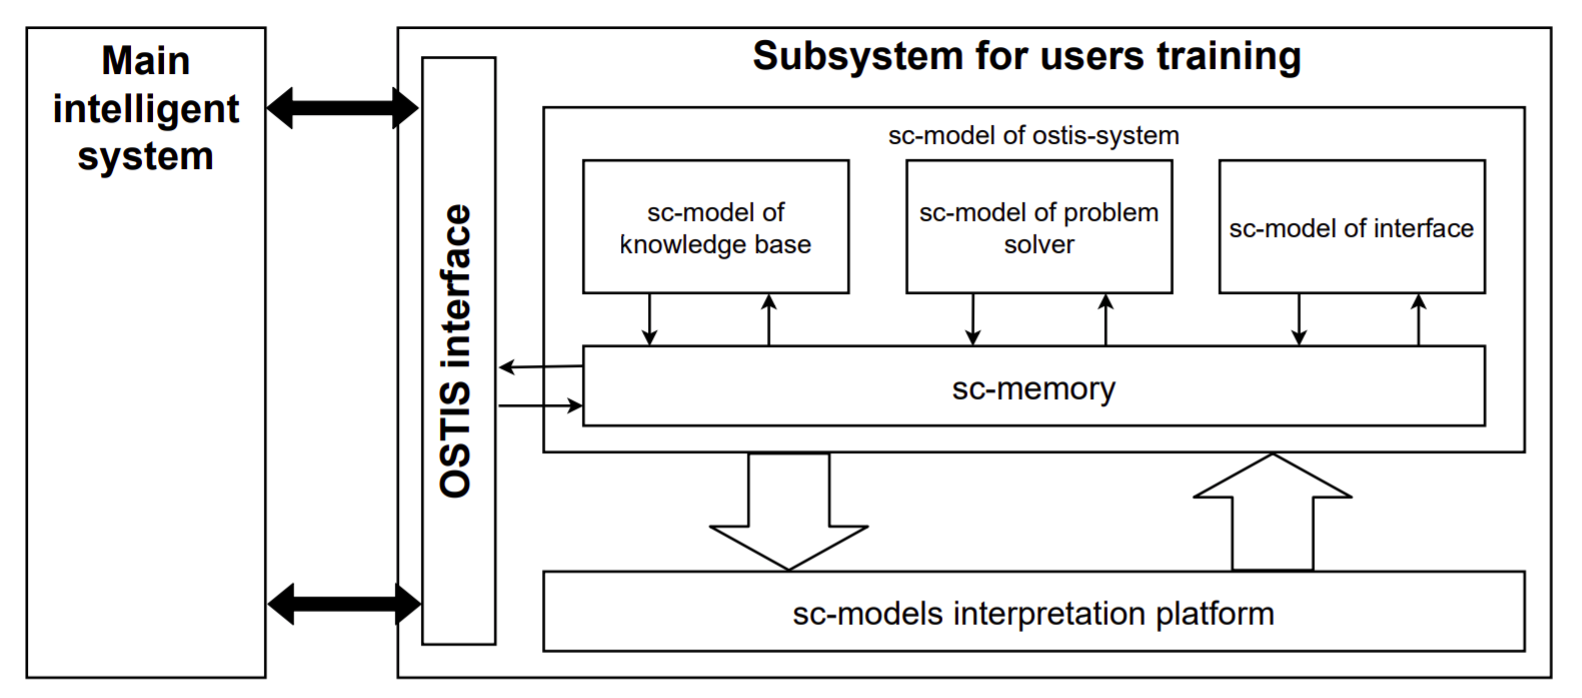
\includegraphics[width=\linewidth]{figures/sd_learning/system_arch.png}}}

\scnnote{В случае, если рассматриваемая интеллектуальная система является \textit{ostis-системой}, ее интеграция с подсистемой обучения пользователей интеллектуальных систем осуществляется более глубоко. Компоненты \textit{подсистемы обучения пользователей интеллектуальных систем} просто дополняют уже существующие в основной ostis-системе компоненты, что позволяет максимально снизить затраты на интеграцию \textit{подсистемы обучения пользователей интеллектуальных систем} и основной \textit{ostis-системы}.}
\scnaddlevel{1}
\scnrelfrom{иллюстрация}{\scnfileimage{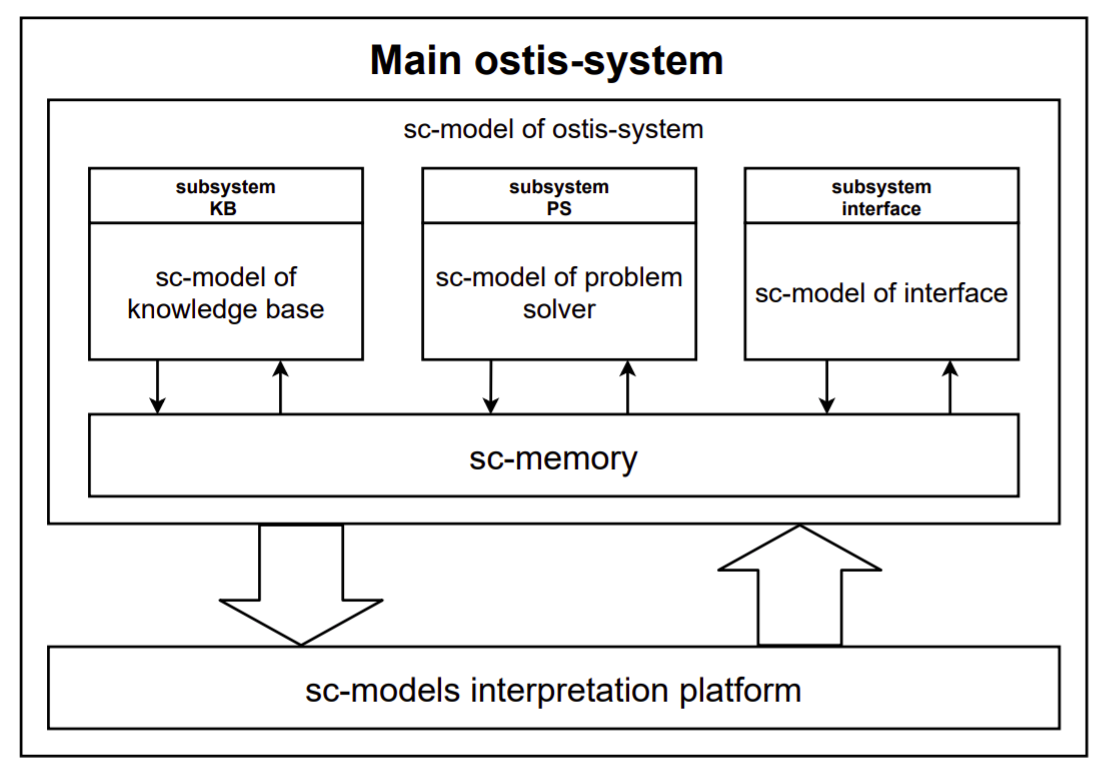
\includegraphics[width=0.8\linewidth]{figures/sd_learning/subsystem_arch.png}}}
\scnaddlevel{-1}
\scnaddlevel{-1}

\scnheader{интеллектуальная обучающая система}
\scnidtf{ИОС}
\scnsubset{интеллектуальная система}
\scnnote{Такого рода системы по сравнению с традиционными системами электронного обучения (например, электронными учебниками) предоставляют обладают рядом существенных преимуществ.}
\scnsubset{интеллектуальная справочная система}
\scnaddlevel{1}
	\scnexplanation{Каждая \textit{интеллектуальная обучающая система} в качестве простейшего средства изучения учебного материала предполагает наличие средств навигации по этому материалу и средств задания по нему различных вопросов. Системы, обладающие только таким ограниченным набором возможностей, названы \textit{интеллектуальными справочными системами}. Таким образом, можно сказать, что \textit{интеллектуальная обучающая система} обязательно реализует в себе функции \textit{интеллектуальной справочной системы}.}
\scnaddlevel{-1}
\scnsuperset{интеллектуальная обучающая ostis-система}
\scnaddlevel{1}
	\scnidtf{интеллектуальная обучающая система, построенная на основе Технологии OSTIS}
\scnaddlevel{-1}

\scnheader{интеллектуальная обучающая ostis-система}
\scnrelfromlist{обобщенная часть}{база знаний интеллектуальной обучающей ostis-системы\\
	\scnaddlevel{1}
	\scnrelfromset{преимущества}{\scnfileitem{SC-код позволяет представлять знания любого рода, в том числе конкретные факты, логические утверждения (аксиомы, теоремы, определения), текстовые и мультимедийные иллюстрации и комментарии, примеры конкретных задач с решениями, в том числе доказательства и т.д.};
	\scnfileitem{Пользователю становятся доступны достаточно полные сведения об изучаемой предметной области, отражены все ее аспекты, благодаря явному помещению в базу знаний всех предметных закономерностей и взаимосвязей понятий.};
	\scnfileitem{База знаний системы рассматривается как иерархия предметных областей и соответствующих им онтологий, то есть позволяет произвести семантическую структуризацию предлагаемого учащемуся материала, что существенно облегчает процесс обучения за счет систематизации знаний на основе именно их семантики, а не каких-либо других сторонних факторов. Кроме этого, знания в базе могут делиться на логические разделы, каждый из которых соответствует какому-либо фрагменту излагаемого материала. База знаний позволяет осуществлять свободную навигацию по любым ассоциативным связям, изучая таким образом материал в той последовательности, какая кажется более логичной для самого обучаемого. С другой стороны, такой подход позволяет указать рекомендуемую последовательность изучения материала. При необходимости структура предметных областей может быть легко перестроена.};
	\scnfileitem{Пользователю в явном виде представляется семантическая структура изучаемого учебного материала и изучаемой предметной области. При этом обеспечивается наглядная визуализация любого уровня указанной семантической структуры.};
	\scnfileitem{Знания из различных областей представляются в сходном виде, что позволяет говорить не о семействе не связанных между собой обучающих систем по различным предметным областям, а о глобальном смысловом пространстве, объединяющем в себе знания всего семейства разрабатываемых систем. В свою очередь, наличие такого смыслового пространства обеспечивает ряд дополнительных возможностей:
	\begin{scnitemize}
		\item каждая система при необходимости может использовать знания, относящиеся к другим системам, что позволяется задавать не только вопросы, касающиеся конкретной предметной области, но и вопросы, носящие междисциплинарный характер;
		\item в рамках глобального смыслового пространства можно выделить часть знаний, которые имеют отношение ко многим системам из всего комплекса, например базовые знания из области математики, логики и т.д. Концепция глобального смыслового пространства позволяет записывать такие фрагменты знаний только в одной из систем, а затем использовать их во всех остальных, что существенно уменьшает количество дублирований, сокращает сроки разработки систем и снижает накладные расходы.
	\end{scnitemize}};
	\scnfileitem{Унифицированное представление знаний позволяет не ограничивать номенклатуру пользовательских запросов только специально выделенными для этого командами, а задавать произвольный запрос системе с использованием универсального языка отображения знаний, что делает перечень возможных запросов зависящим только от количества и разнообразия знаний, внесенных в базу знаний системы.}
	}
	\scnaddlevel{-1}	
	;решатель задач интеллектуальной обучающей ostis-системы\\
	\scnaddlevel{1}
	\scntext{преимущество}{Пользователю предоставляется возможность задавать системе любые вопросы и  задачи по изучаемой предметной области. Это достигается включением в ИОС решателя задач, способного решать задачи по их формулировкам, в том числе, введенным пользователем. При этом указанный решатель задач может находить путь решения задачи даже, если соответствующий способ решения (например, алгоритм) ему неизвестен.}
	\scnaddlevel{-1}	
	;пользовательский интерфейс интеллектуальной обучающей ostis-системы\\
	\scnaddlevel{1}
	\scnrelfromset{преимущества}{
\scnfileitem{Унификация моделей пользовательских интерфейсов позволяет отображать знания различного рода в унифицированном виде независимо от предметной области, к которой эти знания относятся. Таким образом, все разрабатываемые системы будут обладать пользовательским интерфейсом, построенным по одним и тем же принципам, что позволит существенно сократить срок ознакомления учащегося со всем семейством систем. Данный факт не отрицает возможность и необходимость разработки отдельных компонентов интерфейса, ориентированных на конкретную предметную область, например, редактора геометрических чертежей, виртуальной лаборатории для проведения химических опытов и т.д.};
\scnfileitem{ИОС имеет интеллектуальный пользовательский интерфейс с компьютерными (виртуальными) моделями различных объектов изучаемой предметной области, что позволяет системе "понимать"{} смысл (анализировать семантику) пользовательских действий по преобразованию этих объектов. Все это существенно повышает уровень интерактивной виртуальной лабораторной среды электронного учебника.};
\scnfileitem{Каждый компонент пользовательского интерфейса также является отображением определенного элемента из базы знаний, что позволяет, во-первых, легко менять интерфейс системы даже во время ее работы, а, во-вторых, позволяет пользователю задавать системе вопросы не только касательно предметной области, которой посвящена данная система, но и касательно любого из компонентов интерфейса и других частей системы. Таким образом, пользователю достаточно научиться задавать системе несколько простейших вопросов, чтобы в дальнейшем изучить все тонкости работы системой уже в процессе общения с ней.};
\scnfileitem{При общении с системой пользователю предоставляется свобода в выборе любого из множества синонимичных терминов (идентификаторов), зарегистрированных в базе знаний системы. При этом указанные термины могут принадлежать различным естественным языкам.};
\scnfileitem{Появляется принципиальная возможность реализации естественно-языкового интерфейса с пользователем (благодаря широким возможностям семантического анализа пользовательских сообщений и возможностям синтеза на семантическом уровне сообщений, адресуемых пользователям).};
\scnfileitem{Достаточно легко осуществляется переориентация ИОС на обслуживание пользователей с другим естественным языком (т.к. основная часть базы знаний ИОС, непосредственно описывающая семантику соответствующей предметной области, абсолютно не зависит от внешнего  языка, в т.ч. от естественного).}
}
	\scnaddlevel{-1}	
}
\scnrelfromset{преимущества}{
\scnfileitem{Помимо возможности чтения текстов и иллюстративных материалов учебника предоставляется возможность навигации по семантическому пространству предметной области.};
\scnfileitem{Пользователю предоставляется возможность под контролем системы тренироваться (приобретать практические навыки) в решении самых различных задач по изучаемой предметной области. При этом система
\begin{scnitemize}
	\item осуществляет семантический анализ правильности решения задач как по свободно конструируемым ответам (результатам), так и по протоколам решения;
	\item локализует допущенные пользователем ошибки в решении задач, определяет их причину и выдает соответствующие рекомендации пользователю.
\end{scnitemize}};
\scnfileitem{Пользователю предоставляется полная свобода в выборе последовательности изучения учебного материала (маршрута навигации по учебному материалу), но соответствующие рекомендации выдаются.};
\scnfileitem{Пользователю предоставляется полная свобода в выборе решаемых им задач (в сборнике задач и лабораторных работ), но соответствующие рекомендации выдаются. Эти рекомендации направлены на то, чтобы минимизировать число решаемых задач, обеспечивающих приобретение требуемых практических навыков.};
\scnfileitem{В системе не предусматривается специальный режим контроля (проверки, тестирования) знаний. Такой контроль осуществляется незаметно для пользователя путем мониторинга и анализа пользовательских действий при решении им различных задач по изучаемой предметной области. Для этого в базе знаний ИОС имеется информация о том, какие типы задач и лабораторных работ должны быть выполнены пользователем соответственно для удовлетворительного, хорошего и отличного усвоения учебного материала.};
\scnfileitem{Достаточно легко осуществляется интеграция нескольких самостоятельных ИОС по смежным дисциплинам в единый учебник, что, в частности, предоставляет возможность задавать вопросы и задачи на стыке этих дисциплин.};
\scnfileitem{Пользователь ИОС работает под наблюдением и контролем интеллектуального help-а, который помогает пользователю быстро и эффективно освоить возможности системы. По сути это не что иное, как руководство пользователя ИОС, оформленное как семантический электронный учебник.};
\scnfileitem{При проектировании базы знаний ИОС появляется уникальная возможность проверять семантическую корректность формируемого информационного ресурса:
\begin{scnitemize}
	\item корректность определений и утверждений;
	\item корректность использования различных понятий;
	\item корректность алгоритмов;
	\item корректность доказательств теорем;
	\item и т.д.
\end{scnitemize}}
}
\scnaddlevel{1}
\scnnote{Часть из перечисленных возможностей (а в предельном случае и все их них) могут быть реализованы в рамках \textit{подсистемы обучения пользователей интеллектуальных систем}.}
\scnaddlevel{-1}

\scnendstruct \scnendcurrentsectioncomment
\end{SCn}


\scsubsubsection[\scnmonographychapter{Глава 7.4. Интеллектуальные обучающие системы нового поколения}]{Предметная область и онтология дидактических знаний}
\label{sd_didactic}

\scsubsection{Предметная область и онтология семантически совместимых ostis-систем автоматизации проектирования и управления проектированием различных объектов}
\label{sd_management_semantic_comp_sys}

\scsubsection[\scnmonographychapter{Глава 7.6. Умное предприятие и интеллектуальные компьютерные системы нового поколения. Опыт автоматизации предприятия ``Савушкин продукт''}]{Предметная область и онтология семантически совместимых ostis-систем автоматизации производственной деятельности}
\label{sd_activity_semantic_comp_sys}

\scsubsubsection[\scneditors{Крощенко А.А.;Иванюк Д.С.;Пупена А.Н.;Зотов Н.В.;Орлов М.К.}\protect\scnmonographychapter{Глава 7.6. Умное предприятие и интеллектуальные компьютерные системы нового поколения. Опыт автоматизации предприятия “Савушкин продукт”}]{Предметная область и онтология семантически совместимых ostis-систем управления рецептурным производством}
\label{sd_ecosys_enterprise}
\begin{SCn}

\scnsectionheader{\currentname}
\scnstartsubstruct

\scniselement{раздел базы знаний}

\scnheader{Предметная область семантически совместимых ostis-систем управления рецептурным производством}
\scnsdmainclasssingle{***}
\scnsdclass{***}
\scnsdrelation{***}

\bigskip

\scnheader{ostis-система управления рецептурным производством}

\scnendstruct \scnendcurrentsectioncomment

\end{SCn}

\scsubsection[\scneditor{Самодумкин С.А.}\protect\scnmonographychapter{Глава 7.8. Интеллектуальные геоинформационные системы нового поколения}]{Предметная область и онтология геоинформационных ostis-систем}
\label{sd_geosystems}

\scsubsubsection[\scnmonographychapter{Глава 7.8. Интеллектуальные геоинформационные системы нового поколения}]{Предметная область и онтология географических объектов}
\label{sd_geograph_obj}

\scsubsection[\scnmonographychapter{Глава 7.9. Информационная безопасность интеллектуальных компьютерных систем нового поколения}]{Предметная область и онтология средств обеспечения информационной безопасности ostis-систем в рамках Экосистемы OSTIS}
\label{sd_inf_security}